% memorder/memorder.tex

\QuickQuizChapter{chp:memorder:Memory Ordering}{Memory Ordering}
\OriginallyPublished{Chapter}{chp:memorder:Memory Ordering}{Linux Kernel Memory Barriers}{kernel.org}{Howells2009membartxt}
\OriginallyPublished{Chapter}{chp:memorder:Memory Ordering}{A formal kernel memory-ordering model}{Linux Weekly News}{JadeAlglave2017LWN-LKMM-1,JadeAlglave2017LWN-LKMM-2}
%
\Epigraph{The art of progress is to preserve order amid change and to preserve change amid order.}{\emph{Alfred North Whitehead}}

인과성과 순차적 순서는 상당히 직관적이며, 해커들은 일반인들에 비해 이런
개념들을 잘 이해하고 있는 경향을 띄는 경우가 많습니다.
이런 직관들은 순차적 코드와, 락킹과 RCU 같은 표준적 상호배타성 메커니즘을
사용하는 병렬 코드를 작성하고, 분석하고, 디버깅 하는데 매우 강력한 도구가 될 수
있습니다.
불행히도, 표준적 메커니즘을 사용하지 않는 코드에서는 이런 직관들이 깨어지게
되는데, 그런 중요한 예 하나는 이런 표준 메커니즘들을 구현하는 코드입니다.
이 챕터는 동기화 도구들과 다른 성능이 중요한 코드를 구현하기 충분할 만큼
메모리의 순서 규칙에 대해 여러분이 이해할 수 있도록 돕습니다.
\iffalse

Causality and sequencing are deeply intuitive, and hackers often
tend to have a much stronger grasp of these concepts than does
the general population.
These intuitions can be extremely powerful tools when writing, analyzing,
and debugging both sequential code and parallel code that makes
use of standard mutual-exclusion mechanisms, such as locking and
RCU.
Unfortunately, these intuitions break down completely in face of
code that fails to use standard mechanisms, one important example
of course being the code that implements these standard mechanisms.
This chapter will help you gain an understanding of memory ordering
sufficient to implement synchronization primitives and other
performance-critical code.
\fi

@@@ roadmap @@@

\section{Ordering: Why and How?}
\label{sec:memorder:Ordering: Why and How?}

메모리 순서규칙의 필요성이 첫눈에 보면 \co{exists} 절이 절대 발동되지 않을 것을
보장하는 것처럼 보일 수 있는,
Listing~\ref{lst:memorder:Memory Misordering: Store-Buffering Litmus Test}
(\path{C-SB+o-o+o-o.litmus})
으로 보이고 있있습니다.\footnote{
	순수주의자들은 이 \co{exists} 절이 절대 \emph{만족}되지 않는다고
	표현하겠는데, 여기선 assertion 비유를 위해 ``trigger'' 라는 표현을
	사용하겠습니다.}
무엇보다도, \co{exists} 절 안에서 \nbco{0:r2=0} 가 성립된다면,\footnote{
	즉, Thread~\co{P0()} 의 로컬 변수 \co{r2} 의 인스턴스는 0 값을
	갖습니다.
	리트머스 테스트 명명법의 문서를 위해선
	Section~\ref{sec:formal:Anatomy of a Litmus Test} 을 참고하세요.}
우린 Thread~\co{P0()} 의 \co{x1} 로드가 Thread~\co{P1()} 의 \co{x1} 스토어보다
먼저 일어났어야만 한다고 희망하게 되며, 이는 곧 Thread~\co{P1()} 의 \co{x0} 의
로드가 Thread~\co{P0()} 의 \co{x0} 스토어보다 나중에 일어나서 \nbco{1:r2=2}
이어서 \co{exists} 절이 trigger 되지 않게 되길 바라게 됩니다.
이 예제는 대칭적이므로, 비슷한 이유로 \nbco{1:r2=0} 는 \nbco{0:r2=2} 를
보장하길 기대하게 됩니다.
불행히도, 메모리 배리어의 부재는 이런 희망들을 없애버립니다.
CPU 는 비교적 강한 순서 규칙을 갖는 x86 과 같은 시스템에서조차도
Thread~\co{P0()} 와 Thread~\co{P1()} 모두 순서를 바꿀 권한을 가지고 있습니다.
\iffalse

One motivation for memory ordering can be seen in the trivial-seeming
litmus test in
Listing~\ref{lst:memorder:Memory Misordering: Store-Buffering Litmus Test}
(\path{C-SB+o-o+o-o.litmus}),
which at first glance might
appear to guarantee that the \co{exists} clause never triggers.\footnote{
	Purists would instead say that the \co{exists} clause is
	never \emph{satisfied}, but we use ``trigger'' here by
	analogy with assertions.}
After all, if \nbco{0:r2=0} as shown in the \co{exists} clause,\footnote{
	That is, Thread~\co{P0()}'s instance of local variable \co{r2}
	equals zero.
	See Section~\ref{sec:formal:Anatomy of a Litmus Test}
	for documentation of litmus-test nomenclature.}
we might hope that Thread~\co{P0()}'s
load from~\co{x1} must have happened before Thread~\co{P1()}'s store to~\co{x1},
which might raise
further hopes that Thread~\co{P1()}'s load from~\co{x0} must happen after
Thread~\co{P0()}'s store to~\co{x0}, so that \nbco{1:r2=2},
thus not triggering the \co{exists} clause.
The example is symmetric, so similar reasoning might lead
us to hope that \nbco{1:r2=0} guarantees that \nbco{0:r2=2}.
Unfortunately, the lack of memory barriers dashes these hopes.
The CPU is within its rights to reorder
the statements within both Thread~\co{P0()} and Thread~\co{P1()},
even on relatively strongly ordered systems such as x86.
\fi

\begin{listing}[tbp]
{ \scriptsize
\begin{verbbox}[\LstLineNo]
C C-SB+o-o+o-o
{
}

P0(int *x0, int *x1)
{
  int r2;

  WRITE_ONCE(*x0, 2);
  r2 = READ_ONCE(*x1);
}


P1(int *x0, int *x1)
{
  int r2;

  WRITE_ONCE(*x1, 2);
  r2 = READ_ONCE(*x0);
}

exists (1:r2=0 /\ 0:r2=0)
\end{verbbox}
}
\centering
\theverbbox
\caption{Memory Misordering: Store-Buffering Litmus Test}
\label{lst:memorder:Memory Misordering: Store-Buffering Litmus Test}
\end{listing}

\QuickQuiz{}
	컴파일러도
	Listing~\ref{lst:memorder:Memory Misordering: Store-Buffering Litmus Test}
	의 Thread~\co{P0()} 와 Thread~\co{P1()} 의 메모리 액세스 순서를 바꿀 수
	있죠, 그렇죠?
	\iffalse

	The compiler can also reorder Thread~\co{P0()}'s and
	Thread~\co{P1()}'s memory accesses in
	Listing~\ref{lst:memorder:Memory Misordering: Store-Buffering Litmus Test},
	right?
	\fi
\QuickQuizAnswer{
	일반적으로, 컴파일러 최적화는 CPU 가 할 수 있는 것보다 더 극단적이고
	심오한 순서 재배치를 가져옵니다.
	\co{READ_ONCE()} 와 \co{WRITE_ONCE()} 는 컴파일러가 순서를 재배치
	하는걸 막아줍니다.
	그리고 그외에도 많은 걸 막아주기 때문에, 이 섹션에서의 예제들은
	\co{READ_ONCE()} 와 \co{WRITE_ONCE()} 를 많이 사용할 겁니다.
	\iffalse

	In general, compiler optimizations carry out more extensive
	and profound reorderings than CPUs can.
	However, in this case, the volatile accesses in
	\co{READ_ONCE()} and \co{WRITE_ONCE()}
	prevent the compiler from reordering.
	And also from doing much else as well, so the examples in this
	section will be making heavy use of
	\co{READ_ONCE()} and \co{WRITE_ONCE()}.
	% @@@ forward reference to a section describing READ_ONCE()
	% @@@ and WRITE_ONCE().
	\fi
} \QuickQuizEnd

이런 재배치에 대한 의지는
\co{litmus7}~\cite{Alglave:2014:HCM:2594291.2594347} 같은 도구를 통해 확인될 수
있는데, 이 도구는 제 x86 랩탑에서 100,000,000 번의 시도에서 314회 반직관적인
순서가 발생함을 찾아냈습니다.
이상하게 들리겠지만, 두 로드가 모두 값 2 를 리턴하는 경우는 덜 빈번하게
발생했는데, 이 경우엔 167번만 발생했습니다.\footnote{
	이 결과는 실제 하드웨어 구성, 얼마나 시스템에 부하가 가해졌는지,
	그외에도 많은것들에 예민하게 달라질 수 있음을 알아두시기 바랍니다.}
여기서의 교훈은 분명합니다: 증가된 반직관성은 확률의 감소를 의미하지 않습니다!
\iffalse

This willingness to reorder can be confirmed using tools such as
\co{litmus7}~\cite{Alglave:2014:HCM:2594291.2594347},
which found that the counter-intuitive ordering happened
314 times out of 100,000,000 trials on my x86 laptop.
Oddly enough, the perfectly legal outcome where both loads return the
value 2 occurred less frequently, in this case, only 167 times.\footnote{
	Please note that results are sensitive to the exact hardware
	configuration,
	how heavily the system is loaded, and much else besides.}
The lesson here is clear: Increased counterintuitivity does not necessarily
imply decreased probability!
\fi
% Run on June 23, 2017:
% litmus7 -r 1000 -carch X86 C-SB+o-o+o-o.litmus
% Test C-SB+o-o+o-o Allowed
% Histogram (4 states)
% 314   *>0:r2=0; 1:r2=0;
% 49999625:>0:r2=2; 1:r2=0;
% 49999894:>0:r2=0; 1:r2=2;
% 167   :>0:r2=2; 1:r2=2;

다음 섹션들은 이 직관이 정확히 어디서 깨졌는지 보이며, 이어서 여러분이 이런
문제들을 피할 수 있게 도와주는 메모리 배리어의 정신적 모델을 제공합니다.
\iffalse

The following sections show exactly where this intuition breaks down,
and then puts forward a mental model of memory barriers that can help
you avoid these pitfalls.
\fi

Section~\ref{sec:memorder:Why Hardware Misordering?}
왜 하드웨어 가 메모리 액세스들의 순서를 잘못 잡는지에 대한 짧은 소개를
제공하고, 이어서
Section~\ref{sec:memorder:How to Force Ordering?}
에서는 어떻게 여러분이 악의 사악한 하드웨어의 순서를 잘못잡는 계획을 좌절시킬
수 있는지에 대해 마찬가지로 짧은 소개를 제공합니다.
마지막으로, Section~\ref{sec:memorder:Basic Rules of Thumb} 은 뒤의 섹션들에서
더 잘 다듬어질 경험으로부터의 법칙들을 보입니다.
\iffalse

Section~\ref{sec:memorder:Why Hardware Misordering?}
gives a brief overview of why hardware misorders memory accesses, and then
Section~\ref{sec:memorder:How to Force Ordering?}
gives an equally brief overview of how you can thwart evil hardware
misordering schemes.
Finally, Section~\ref{sec:memorder:Basic Rules of Thumb}
lists some basic rules of thum, which will be further refined in
later sections.
\fi

\subsection{Why Hardware Misordering?}
\label{sec:memorder:Why Hardware Misordering?}

하지만 대체 왜 메모리 배리어가 필요한거죠?
CPU 는 스스로 순서를 기록하고 있을 수 없는 건가요?
일단 그게 바로 우리가 어떤 것들을 기록하고 있기 위해 컴퓨터를 갖는 이유이지
않던가요?
\iffalse

But why are memory barriers needed in the first place?
Can't CPUs keep track of ordering on their own?
Isn't that why we have computers in the first place, to keep track of things?
\fi

많은 사람들이 실제로 자신의 컴퓨터가 사물에 대해 기록을 가지고 있을 것이라
기대합니다만, 많은 사람들은 또한 그 기록을 빠르게 관리할 것을 요구합니다.
하지만, Chapter~\ref{chp:Hardware and its Habits} 에서 보였듯이, 근래의 컴퓨터
시스템 제조사들이 직면한 어려움 중 한가지는 메인 메모리가 CPU 의 속도 향상을
따라가지 못한다는 것입니다---근래의 CPU 들은 메모리로부터 변수 하나의 값을
읽어오는데 필요한 시간 동안 수백개의 명령어를 실행할 수 있습니다.
따라서 CPU 들은
Figure~\ref{fig:cpu:System Hardware Architecture} 에서 보인 것과 같이
갈수록 커다란 캐시들을 갖추는데, 이는 특정 CPU 의 특정 변수로부터의 첫번째
로드가
Section~\ref{sec:cpu:Cache Misses} 에서 이야기한 값비싼 \emph{캐시 미스} 를
낸다 하더라도, 최초의 캐시 미스는 해당 변수가 해당 CPU 의 캐시에 올라오게 하기
때문에 해당 CPU 로부터 해당 변수로의 뒤이은 반복된 로드들은 매우 빠르게
수행될 수도 있음을 의미합니다.
\iffalse

Many people do indeed expect their computers to keep track of things,
but many also insist that they keep track of things quickly.
However, as seen in Chapter~\ref{chp:Hardware and its Habits},
one difficulty that modern computer-system vendors face is that
the main memory cannot keep up with the CPU---modern CPUs can execute
hundreds of instructions in the time required to fetch a single variable
from memory.
CPUs therefore sport increasingly large caches, as seen back in
Figure~\ref{fig:cpu:System Hardware Architecture}, which means that
although the first load by a given CPU from a given variable will
result in an expensive \emph{cache miss} as was discussed in
Section~\ref{sec:cpu:Cache Misses}, subsequent
repeated loads from that variable by that CPU might execute
very quickly because the initial cache miss will have loaded that
variable into that CPU's cache.
\fi

하지만, 여러 CPU 들로부터 공유된 변수들 집합으로 이루어지는 빈번한 동시적
스토어들을 잘 처리할 필요 또한 있습니다.
Cache-coherent 시스템에서, 캐시들이 특정 변수의 여러 복사본들을 가지고 있다면,
이 모든 복사본들은 같은 값을 가져야만 합니다.
이는 동시의 로드들에 대해서는 매우 잘 동작하지만, 동시의 스토어들에 대해서는
그렇지 못합니다:  각각의 스토어는 기존 값의 복사본들 모두에 대해서 어떤 일을
해줘야 하는데 (또다른 캐시 미스!), 이는 빛의 제한된 속도와 원자적 물질의 원리를
놓고 보면, 성급한 소프트웨어 해커들이 좋아하지 않을 만큼 느릴 겁니다.
\iffalse

However, it is also necessary to accommodate frequent concurrent stores
from multiple CPUs to a set of shared variables.
In cache-coherent systems, if the caches hold multiple copies of a given
variable, all the copies of that variable must have the same value.
This works extremely well for concurrent loads, but not so well for
concurrent stores:  Each store must do something about all
copies of the old value (another cache miss!), which, given the finite
speed of light and the atomic nature of matter, will be slower
than impatient software hackers would like.
\fi

\begin{figure}[tb]
\centering
\resizebox{2.5in}{!}{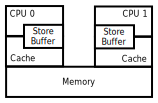
\includegraphics{memorder/SystemArchSB}}
\caption{System Architecture With Store Buffers}
\label{fig:memorder:System Architecture With Store Buffers}
\end{figure}

따라서 CPU 들은
Figure~\ref{fig:memorder:System Architecture With Store Buffers} 에 보인 것처럼
스토어 버퍼를 장착합니다.
특정 CPU 가 특정 변수에 스토어를 수행하는데 해당 변수가 해당 CPU 의 캐시에
존재하지 않는다면, 이 새로운 값은 해당 CPU 의 스토어 버퍼에 저장됩니다.
이 CPU 는 이제 이 스토어가 다른 CPU 들의 캐시들에 있을 수 있는 이 변수의 기존
값에 뭔가 작업을 수행할동안 기다리지 않고 곧바로 작업을 진행할 수 있습니다.
\iffalse

CPUs therefore come equipped with store buffers, as shown in
Figure~\ref{fig:memorder:System Architecture With Store Buffers}.
When a given CPU does a store to a variable that
is not present in that CPU's cache, then the new value
is instead placed in that CPU's store buffer.
The CPU can then proceed immediately, without having to wait for the
store to do something about all the old values of that variable
residing in other CPUs' caches.
\fi

\begin{figure}[htb]
\centering
\resizebox{3in}{!}{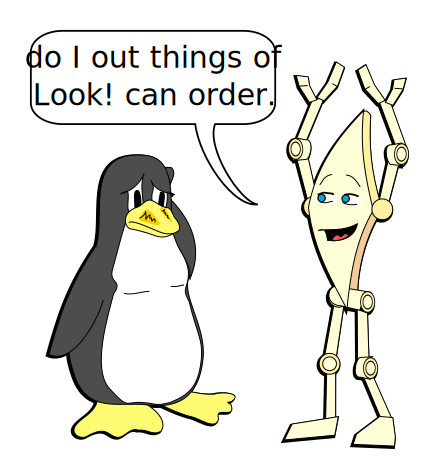
\includegraphics{cartoons/r-2014-Out-of-order}}
\caption{CPUs Can Do Things Out of Order}
\ContributedBy{Figure}{fig:memorder:CPUs Can Do Things Out of Order}{Melissa Broussard}
\end{figure}

스토어 버퍼들이 성능을 상당히 향상시킬 수 있지만, 이것들은 인스트럭션들과
메모리 참조들이 비순차적으로 수행되게 만들 수 있는데, 이는 곧 심각한 혼란을
가져오게 되는데, 이 상황이
Figure~\ref{fig:memorder:CPUs Can Do Things Out of Order} 에 그려져 있습니다.
구체적으로는, 이런 스토어 버퍼들이
Listing~\ref{lst:memorder:Memory Misordering: Store-Buffering Litmus Test} 에
보인 스토어 버퍼 리트머스 테스트에 보인 잘못된 메모리 순서를 가능하게 할 수
있습니다.
\iffalse

Although store buffers can greatly increase performance,
they can cause instructions and memory references to execute out
of order, which can in turn cause serious confusion, as illustrated in
Figure~\ref{fig:memorder:CPUs Can Do Things Out of Order}.
In particular, these store buffers can cause the memory misordering
shown in the store-buffering litmus test in
Listing~\ref{lst:memorder:Memory Misordering: Store-Buffering Litmus Test}.
\fi

\begin{table*}
\small
\centering\OneColumnHSpace{-0.1in}
\begin{tabular}{r||l|l|l||l|l|l}
	& \multicolumn{3}{c||}{CPU 0} & \multicolumn{3}{c}{CPU 1} \\
	\cline{2-7}
	& Instruction & Store Buffer & Cache &
		Instruction & Store Buffer & Cache \\
	\hline
	\hline
	1 & (Initial state) & & \tco{x1==0} &
		(Initial state) & & \tco{x0==0} \\
	\hline
	2 & \tco{x0 = 2;} & \tco{x0==2} & \tco{x1==0} &
		\tco{x1 = 2;} & \tco{x1==2} & \tco{x0==0} \\
	\hline
	3 & \tco{r2 = x1;} (0) & \tco{x0==2} & \tco{x1==0} &
		\tco{r2 = x0;} (0) & \tco{x1==2} & \tco{x0==0} \\
	\hline
	4 & (Read-invalidate) & \tco{x0==2} & \tco{x0==0} &
		(Read-invalidate) & \tco{x1==2} & \tco{x1==0} \\
	\hline
	5 & (Finish store) & & \tco{x0==2} &
		(Finish store) & & \tco{x1==2} \\
\end{tabular}
\caption{Memory Misordering: Store-Buffering Sequence of Events}
\label{tab:memorder:Memory Misordering: Store-Buffering Sequence of Events}
\end{table*}

Table~\ref{tab:memorder:Memory Misordering: Store-Buffering Sequence of Events}
은 이런 잘못된 메모리 접근 순서가 어떻게 일어날 수 있는지 보입니다.
Row~1 은 최초의 상태를 보이는데, 이 때 CPU~0 는 \co{x1} 을 자신의 캐시에 가지고
있고 CPU~1 은 \co{x0} 를 자기의 캐시에 가지고 있으며, 두 변수 모두 값 0을
가지고 있습니다.
Row~2 는 각 CPU 의 스토어 (
Listing~\ref{lst:memorder:Memory Misordering: Store-Buffering Litmus Test} 의
line~9 와~18) 로 인한 상태 변화를 보입니다.
두 CPU 모두 스토어가 향한 변수를 자신의 캐시에 가지고 있지 않았기에, 두 CPU 는
모두 각자의 스토어들을 자신의 스토어 버퍼들에서 처리합니다.
\iffalse

Table~\ref{tab:memorder:Memory Misordering: Store-Buffering Sequence of Events}
shows how this memory misordering can happen.
Row~1 shows the initial state, where CPU~0 has \co{x1} in its cache
and CPU~1 has \co{x0} in its cache, both variables having a value of zero.
Row~2 shows the state change due to each CPU's store (lines~9 and~18 of
Listing~\ref{lst:memorder:Memory Misordering: Store-Buffering Litmus Test}).
Because neither CPU has the stored-to variable in its cache, both CPUs
record their stores in their respective store buffers.
\fi

\QuickQuiz{}
	하지만 잠시만요!!!
	Table~\ref{tab:memorder:Memory Misordering: Store-Buffering Sequence of Events}
	의 row~2 에서 \co{x0} 와 \co{x1} 모두 동시에 두개의 값, 0 과 1 을
	가지고 있어요.
	어떻게 이게 가능한거죠???
	\iffalse

	But wait!!!
	On row~2 of
	Table~\ref{tab:memorder:Memory Misordering: Store-Buffering Sequence of Events}
	both \co{x0} and \co{x1} each have two values at the same time,
	namely zero and two.
	How can that possibly work???
	\fi
\QuickQuizAnswer{
	나중에 이야기 하겠지만, 아래쪽에 좀 더 일을 빠듯하게 처리되도록 하는
	cache-coherence 프로토콜이 존재합니다.
	하지만 어떤 변수가 동시에 두개의 값을 갖는다는게 신기하다고
	생각하신다면,
	Section~\ref{sec:memorder:Variables With Multiple Values} 까지
	잠깐 기다려 주시기 바랍니다.
	\iffalse

	There is an underlying cache-coherence protocol that straightens
	things out, which will be discussed later.
	% @@@ Add forward reference.
	But if you think that a given variable having two values at
	the same time is surprising, just wait until you get to
	Section~\ref{sec:memorder:Variables With Multiple Values}!
	\fi
} \QuickQuizEnd

Row~3 는 두개의 로드
(Listing~\ref{lst:memorder:Memory Misordering: Store-Buffering Litmus Test} 의
line~10 과~19) 를 보입니다.
각 CPU 에 의해 읽혀지는 변수들은 각 CPU 의 캐시에 있기 때문에, 각각의 로드는
곧바로 캐시의 값을 반환하는데, 이 경우 모두 0의 값입니다.

하지만 이 CPU 들은 일이 다 끝나지 않았습니다: 금방이든 나중이든, 각자의 스토어
버퍼를 비워야만 합니다.
캐시는 \emph{캐시라인 (cacheline)} 이라 불리는 상대적으로 커다란 블록 단위로
데이터를 옮기기 때문에, 그리고 각각의 캐시라인은 여러 변수들을 담고 있을 수
있기 때문에, 각 CPU 는 자신의 스토어 버퍼 안의 변수에 해당하는 캐시라인의 해당
변수에 해당하지 않는 부분은 만지지 않으면서 해당 변수에 해당하는 부분만을
업데이트 할 수 있도록 해당 캐시라인을 자신의 캐시로 가져와야만 합니다.
각 CPU 는 또한 해당 캐시라인이 어떤 다른 CPU 의 캐시에도 존재하지 않는다는 점을
보장해야만 하는데, 이를 위해 read-invalidate 오퍼레이션이 사용됩니다.
Row~4 에서 보인 것처럼, 두개의 read-invalidate 오퍼레이션이 완료된 후, 이 두
CPU 는 서로 넘겨받은 캐시라인들을 가지고 있게 되어서, CPU~0 의 캐시는 이제
\co{x0} 를 담고 있고 CPU~1 의 캐시는 \co{x1} 을 담고 있게 됩니다.
일단 이 두 변수들이 각자의 새로운 안식처에 위치하게 되면, 각 CPU 는 자신의
스토어 버퍼를 연관된 캐시 라인으로 비워낼 수 있게 되어서, 각 변수의 값을 row~5
에 보인 대로 마지막 값으로 설정합니다.
\iffalse

Row~3 shows the two loads (lines~10 and~19 of
Listing~\ref{lst:memorder:Memory Misordering: Store-Buffering Litmus Test}).
Because the variable being loaded by each CPU is in that CPU's cache,
each load immediately returns the cached value, which in both cases
is zero.

But the CPUs are not done yet: Sooner or later, they must empty their
store buffers.
Because caches move data around in relatively large blocks called
\emph{cachelines}, and because each cacheline can hold several
variables, each CPU must get the cacheline into its own cache so
that it can update the portion of that cacheline corresponding
to the variable in its store buffer, but without disturbing any
other part of the cacheline.
Each CPU must also ensure that the cacheline is not present in any other
CPU's cache, for which a read-invalidate operation is used.
As shown on row~4, after both read-invalidate operations complete,
the two CPUs have traded cachelines, so that CPU~0's cache now contains
\co{x0} and CPU~1's cache now contains \co{x1}.
Once these two variables are in their new homes, each CPU can flush
its store buffer into the corresponding cache line, leaving each
variable with its final value as shown on row~5.
\fi

\QuickQuiz{}
	하지만 이 값들은 또다시 캐시에서 메인 메모리로 비워져야 하는거
	아닌가요?
	\iffalse

	But don't the values also need to be flushed from the cache
	to main memory?
	\fi
\QuickQuizAnswer{
	놀라울 수 있겠지만, 꼭 그럴 필요는 없습니다!
	어떤 시스템들에서는, 두개의 변수들이 빈번하게 사용된다면, 이 변수들은
	CPU 의 캐시들 사이에서 움직이게 되고 메인 메모리에는 위치하지 않게
	됩니다.
	\iffalse

	Perhaps surprisingly, not necessarily!
	On some systems,
	if the two variables are being used heavily, they might
	be bounced back and forth between the CPUs' caches and never
	land in main memory.
	\fi
} \QuickQuizEnd

요약하자면, 스토어 버퍼들은 CPUe 들이 스토어 명령을 효과적으로 처리할 수 있도록
하기 위해 필요합니다만, 이게 반 직관적인, 잘못된 메모리 접근 순서를 야기할 수
있습니다.

하지만 여러분의 알고리즘이 정말로 메모리 참조의 순서를 맞춰야 한다면 어떻게
해야할까요?
예를 들어, 여러분이 어떤 드라이버와 하나는 이 드라이버가 동작 중인지 여부를 말하고 (driver-running flag) 하나는 이 드라이버에 처리되기를 기다리는 중인 요청이 있는지 여부를 말하는 (request-pending flag) 한쌍의 플래그를 사용해 통신하고 있다고 생각해 봅시다.
요청을 보내는 쪽은 request-pending flag 의 bit 을 채우고, driver-running flag 의 bit 을 검사한 후, 비어있다면 드라이버를 깨웁니다.
드라이버가 자신이 아는 모든 대기중인 요청들을 처리했다면, 드라이버는 자신의 driver-running flag 의 bit 을 없애고, 다시 일을 시작해야 하는지 여부를 보기 위해 request-pending flag 를 체크해야 합니다.
이 매우 합리적인 접근법도 하드웨어가 여기서의 스토어들과 로드들을 순서대로 처리한다고 보장할 수 있는 방법이 없다면 제대로 동작하지 않을 겁니다.
이게 다음 섹션의 주제입니다.
\iffalse

In summary, store buffers are needed to allow CPUs to handle
store instructions efficiently, but they can result in
counter-intuitive memory misordering.

But what do you do if your algorithm really needs its memory
references to be ordered?
For example, suppose that you are communicating with a driver using
a pair of flags, one that says whether or not the driver is running
and the other that says whether there is a request pending for that
driver.
The requester needs to set the request-pending flag, then check
the driver-running flag, and if false, wake it up.
Once the driver has serviced all the pending requests that it knows about,
it needs to clear its driver-running flag, then check the request-pending
flag to see if it needs to restart.
This very reasonable approach cannot work unless there is some way
to make sure that the hardware processes the stores and loads in order.
This is the subject of the next section.
\fi

\subsection{How to Force Ordering?}
\label{sec:memorder:How to Force Ordering?}

\emph{메모리 배리어} (예를 들어, 리눅스 커널의 \co{smp_mb()}) 를 사용해 순서
규칙의 환상을 지키는데 필요한 표준적 동기화 도구들 (락킹과 RCU 같은) 과
컴파일러 지시어들이 존재합니다.
이런 메모리 배리어들은 ARM, POWER, Itanium, 그리고 Alpha 에서처럼 명시적
인스트럭션이 될 수 있고, x86 에서 종종 그런 것처럼 다른 인스트럭션들에 의해
내포될 수도 있습니다.
이런 표준적 동기화 도구들은 순서가 지켜진다는 환상을 지키기 때문에, 여러분이
가장 쉽게 적용할 수 있는 방법은 그냥 이 도구들을 사용해서, 이 섹션을 그만 읽는
겁니다.
\iffalse

It turns out that there are compiler directives and standard
synchronization primitives (such as locking and RCU)
that are responsible for maintaining the illusion of ordering through use of
\emph{memory barriers} (for example, \co{smp_mb()} in the Linux kernel).
These memory barriers can be explicit instructions, as they are on
ARM, POWER, Itanium, and Alpha, or they can be implied by other instructions,
as they often are on x86.
Since these standard synchronization primitives preserve the illusion of
ordering, your path of least resistance is to simply use these primitives,
thus allowing you to stop reading this section.
\fi

\begin{listing}[tbp]
{ \scriptsize
\begin{verbbox}[\LstLineNo]
C C-SB+o-mb-o+o-mb-o
{
}

P0(int *x0, int *x1)
{
  int r2;

  WRITE_ONCE(*x0, 2);
  smp_mb();
  r2 = READ_ONCE(*x1);
}


P1(int *x0, int *x1)
{
  int r2;

  WRITE_ONCE(*x1, 2);
  smp_mb();
  r2 = READ_ONCE(*x0);
}

exists (1:r2=0 /\ 0:r2=0)
\end{verbbox}
}
\centering
\theverbbox
\caption{Memory Ordering: Store-Buffering Litmus Test}
\label{lst:memorder:Memory Ordering: Store-Buffering Litmus Test}
\end{listing}

하지만, 여러분 스스로 그런 동기화 도구들을 구현해야 한다면, 또는 그런 메모리
순서 규칙과 메모리 배리어가 어떻게 동작하는지에 그저 흥미가 있는 거라면, 계속
읽어주세요!
이 여정에서의 첫번째 정류장은
Listing~\ref{lst:memorder:Memory Ordering: Store-Buffering Litmus Test}
(\path{C-SB+o-mb-o+o-mb-o.litmus}) 으로, \co{smp_mb()} 리눅스 커널 메모리
배리어가 \co{P0()} 와 \co{P1()} 의 스토어와 로드 사이에 위치했다는 점을
제외하고는
Listing~\ref{lst:memorder:Memory Misordering: Store-Buffering Litmus Test}
와 동일합니다.
이 배리어들은 제 x86 랩탑에서의 100,000,000 번의 시도에도 반 직관적인 결과가
일어나는 것을 막았습니다.
흥미롭게도, 이 배리어들로 인해 추가된 오버헤드는 두 로드가 모두 값 2 를
반환하는 경우가 800,000 번이 넘게 일어나게 만들었는데, 이는 이 배리어가 없는
Listing~\ref{lst:memorder:Memory Misordering: Store-Buffering Litmus Test} 의
코드에서는 167 번밖에 일어나지 않았던 것과 대조적입니다.
\iffalse

However, if you need to implement the synchronization primitives
themselves, or if you are simply interested in understanding how memory
ordering and memory barriers work, read on!
The first stop on the journey is
Listing~\ref{lst:memorder:Memory Ordering: Store-Buffering Litmus Test}
(\path{C-SB+o-mb-o+o-mb-o.litmus}),
which places an \co{smp_mb()} Linux-kernel full memory barrier between
the store and load in both \co{P0()} and \co{P1()}, but is otherwise
identical to
Listing~\ref{lst:memorder:Memory Misordering: Store-Buffering Litmus Test}.
% Test C-SB+o-mb-o+o-mb-o Allowed
% Histogram (3 states)
% 49553298:>0:r2=2; 1:r2=0;
% 49636449:>0:r2=0; 1:r2=2;
% 810253:>0:r2=2; 1:r2=2;
% No
These barriers prevent the counter-intuitive outcome from happening
on 100,000,000 trials on my x86 laptop.
Interestingly enough, the added overhead due to these barriers causes the
legal outcome where both loads return the value two to happen more
than 800,000 times, as opposed to only 167 times for the
barrier-free code in
Listing~\ref{lst:memorder:Memory Misordering: Store-Buffering Litmus Test}.
\fi

\begin{table*}
\small
\centering\OneColumnHSpace{-0.1in}
\begin{tabular}{r||l|l|l||l|l|l}
	& \multicolumn{3}{c||}{CPU 0} & \multicolumn{3}{c}{CPU 1} \\
	\cline{2-7}
	& Instruction & Store Buffer & Cache &
		Instruction & Store Buffer & Cache \\
	\hline
	\hline
	1 & (Initial state) & & \tco{x1==0} &
		(Initial state) & & \tco{x0==0} \\
	\hline
	2 & \tco{x0 = 2;} & \tco{x0==2} & \tco{x1==0} &
		\tco{x1 = 2;} & \tco{x1==2} & \tco{x0==0} \\
	\hline
	3 & \tco{smp_mb();} & \tco{x0==2} & \tco{x1==0} &
		\tco{smp_mb();} & \tco{x1==2} & \tco{x0==0} \\
	\hline
	4 & (Read-invalidate) & \tco{x0==2} & \tco{x0==0} &
		(Read-invalidate) & \tco{x1==2} & \tco{x1==0} \\
	\hline
	5 & (Finish store) & & \tco{x0==2} &
		(Finish store) & & \tco{x1==2} \\
	\hline
	6 & \tco{r2 = x1;} (2) & & \tco{x1==2} &
		\tco{r2 = x0;} (2) & & \tco{x0==2} \\
\end{tabular}
\caption{Memory Ordering: Store-Buffering Sequence of Events}
\label{tab:memorder:Memory Ordering: Store-Buffering Sequence of Events}
\end{table*}

이 배리어들은
Table~\ref{tab:memorder:Memory Ordering: Store-Buffering Sequence of Events} 에
보인 것과 같이 순서규칙에 깊은 영향을 끼칩니다.
앞의 두 행은
Table~\ref{tab:memorder:Memory Misordering: Store-Buffering Sequence of Events}
에 보인 것과 같고 row~3 의 \co{smp_mb()} 인스트럭션들은 직접적으로 상태를
바꾸지 않지만, 이 인스트럭션들은 스토어들이 (row~4 와~5) 로드 (row~6) 전에
완료되도록 만들어서,
Table~\ref{tab:memorder:Memory Misordering: Store-Buffering Sequence of Events}
에서 보인 반 직관적인 결과가 나타나지 못하게 합니다.
변수 \co{x0} 와 \co{x1} 은 row~2 에서 여전히 두개의 값을 갖지만, 앞서
약속한대로, 이 \co{smp_mb()} 인스턴스들은 최종적으로는 일을 더 깐깐하게
처리했음을 알아두시기 바랍니다.
\iffalse

These barriers have a profound effect on ordering, as can be seen in
Table~\ref{tab:memorder:Memory Ordering: Store-Buffering Sequence of Events}.
Although the first two rows are the same as in
Table~\ref{tab:memorder:Memory Misordering: Store-Buffering Sequence of Events}
and although the \co{smp_mb()} instructions on row~3
do not change state
in and of themselves, they do cause the stores to complete
(rows~4 and~5) before the
loads (row~6), which rules out the counter-intuitive outcome shown in
Table~\ref{tab:memorder:Memory Misordering: Store-Buffering Sequence of Events}.
Note that variables \co{x0} and \co{x1} each still have more than one
value on row~2, however, as promised earlier, the \co{smp_mb()}
instances straighten things out in the end.
\fi

\begin{table*}
\small
\centering\OneColumnHSpace{-0.7in}
\begin{tabular}{l||c||c|c|c|c||c|c|c|c|c|c|c}
	& & \multicolumn{4}{c||}{Prior Ordered Operation} &
		\multicolumn{7}{c}{Subsequent Ordered Operation} \\
	\cline{3-6} \cline{7-13}
	Operation Providing Ordering & C &
		Self & R & W & RMW & Self & R & W & DR & DW & RMW & SV \\
	\hline
	\hline
	Store, for example, \tco{WRITE_ONCE()} &  &
		   Y &   &   &     &      &   &   &    &    &     &  Y \\
	\hline
	Load, for example, \tco{READ_ONCE()} &  &
		   Y &   &   &     &      &   &   &    &  Y &     &  Y \\
	\hline
	Unsuccessful RMW operation &  &
		   Y &   &   &     &      &   &   &    &  Y &     &  Y \\
	\hline
	\tco{smp_read_barrier_depends()} &  &
		     & Y &   &     &      &   &   &  Y &  Y &     &    \\
	\hline
	\tco{*_dereference()} &  &
		   Y &   &   &     &      &   &   &  Y &  Y &     &  Y \\
	\hline
	Successful \tco{*_acquire()} &   &
		   R &   &   &     &      & Y & Y &  Y &  Y &   Y &  Y \\
	\hline
	Successful \tco{*_release()} & C &
		     & Y & Y &   Y &    W &   &   &    &    &     &  Y \\
	\hline
	\tco{smp_rmb()} &   &
		     & Y &   &   R &      & Y &   &  Y &    &   R &    \\
	\hline
	\tco{smp_wmb()} &   &
		     &   & Y &   W &      &   & Y &    &  Y &   W &    \\
	\hline
	\tco{smp_mb()} & CP &
		     & Y & Y &   Y &      & Y & Y &  Y &  Y &   Y &    \\
	\hline
	Successful full-strength non-\tco{void} RMW & CP &
		   Y & Y & Y &   Y &    Y & Y & Y &  Y &  Y &   Y &  Y \\
	\hline
	\tco{smp_mb__before_atomic()} & CP &
		     & Y & Y &   Y &      & a & a & a  & a  &   Y &    \\
	\hline
	\tco{smp_mb__after_atomic()} & CP &
		     & a & a &   Y &      & Y & Y &  Y &  Y &     &    \\
	\multicolumn{13}{c}{~} \\
	\multicolumn{1}{r}{Key:} &
		\multicolumn{12}{l}{C: Ordering is cumulative} \\
	\multicolumn{1}{r}{} &
		\multicolumn{12}{l}{P: Ordering propagates} \\
	\multicolumn{1}{r}{} &
		\multicolumn{12}{l}{R: Read, for example, \tco{READ_ONCE()}, or read portion of RMW} \\
	\multicolumn{1}{r}{} &
		\multicolumn{12}{l}{W: Write, for example, \tco{WRITE_ONCE()}, or write portion of RMW} \\
	\multicolumn{1}{r}{} &
		\multicolumn{12}{l}{Y: Provides the specified ordering} \\
	\multicolumn{1}{r}{} &
		\multicolumn{12}{l}{a: Provides specified ordering given intervening RMW atomic operation} \\
	\multicolumn{1}{r}{} &
		\multicolumn{12}{l}{DR: Dependent read (address dependency, Section~\ref{sec:memorder:Address Dependencies})} \\
	\multicolumn{1}{r}{} &
		\multicolumn{12}{l}{DW: Dependent write (address, data, or control dependency, Sections~\ref{sec:memorder:Address Dependencies}--\ref{sec:memorder:Control Dependencies})} \\
	\multicolumn{1}{r}{} &
		\multicolumn{12}{l}{RMW: Atomic read-modify-write operation} \\
	\multicolumn{1}{r}{} &
		\multicolumn{12}{l}{SV: Same-variable access} \\
\end{tabular}
\caption{Linux-Kernel Memory-Ordering Cheat Sheet}
\label{tab:memorder:Linux-Kernel Memory-Ordering Cheat Sheet}
\end{table*}

\co{smp_mb()} 가 상당히 강력한 순서 보장을 갖긴 하지만, 그 강력함은 높은
비용으로부터 나옵니다.
굉장히 많은 상황들이 저렴한 메모리 배리어 인스트럭션을 사용하는, 또는, 어떤
경우에 있어서는, 아예 메모리 배리어 인스트럭션을 사용하지 않는 훨씬 약한 순서
보장만으로도 처리될 수 있습니다.
Table~\ref{tab:memorder:Linux-Kernel Memory-Ordering Cheat Sheet}
은 리눅스 커널의 순서 보장 도구들과 그 보장사항들을 보이는 커닝 페이퍼를
보입니다.
각 열은 순서 보장을 제공할 수도, 하지 않을 수도 있는 도구들 또는 도구들의
카테고리에 연관되며, ``Prior Ordered Operation'' 과 ``Subsequent Ordered
Operation'' 으로 라벨링된 행들은 각 열의 도구에 의해 순서가 맞춰지는 (또는
맞춰지지 않는) 오퍼레이션들입니다.
``Y'' 를 담는 셀들은 무조건적으로 순서가 제공됨을 의미하며, 다른 문자들은
순서가 부분적으로 또는 조건적으로 제공됨을 의미합니다.
빈 셀들은 어떤 순서 보장도 제공되지 않음을 의미합니다.
\iffalse

Although \co{smp_mb()} has extremely strong ordering guarantees, its strength
comes at a high price.
A great many situations can be handled with much weaker ordering guarantees
that use much cheaper memory-barrier instructions, or, in some case, no
memory-barrier instructions at all.
Table~\ref{tab:memorder:Linux-Kernel Memory-Ordering Cheat Sheet}
provides a cheatsheet of the Linux kernel's ordering primitives and their
guarantees.
Each row corresponds to a primitive or category of primitives that might
or might not provide ordering, with the columns labeled
``Prior Ordered Operation'' and ``Subsequent Ordered Operation''
being the operations that might (or might not) be ordered against.
Cells containing ``Y'' indicate that ordering is supplied unconditionally,
while other characters indicate that ordering is supplied only partially or
conditionally.
Blank cells indicate that no ordering is supplied.
\fi

\co{*_acquire} 열은 \co{smp_load_acquire()}, \co{cmpxchg_acquire()},
\co{xchg_release()}, 등등을 포함합니다;
\co{*_release} 열은 \co{smp_store_release()}, \co{cmpxchg_release()},
\co{xchg_release()}, 등등을 포함합니다; 그리고
``Successful Non-Relaxed Non-\co{void} RMW'' 열은 \co{atomic_add_return()},
\co{atomic_add_unless()}, \co{atomic_dec_and_test()}, \co{cmpxchg()},
\co{xchg()}, 등등을 포함합니다.
``Successful'' 이라는 수식어는 앞의 ``Unsuccessful RMW operation'' 행에서도
가리키듯이, 실패했을 때에는 메모리에도 순서에도 어떤 영향을 끼치지 않는
\co{atomic_add_return()}, \co{cmpxchg_acquire()}, 그리고 \co{cmpxchg_release()}
같은 도구들에 적용됩니다.
\iffalse

The \co{*_acquire} row covers \co{smp_load_acquire()},
\co{cmpxchg_acquire()}, \co{xchg_release()}, and so on;
the \co{*_release} row covers \co{smp_store_release()},
\co{cmpxchg_release()}, \co{xchg_release()}, and so on; and
the ``Successful Non-Relaxed Non-\co{void} RMW'' row covers
\co{atomic_add_return()}, \co{atomic_add_unless()}, \co{atomic_dec_and_test()},
\co{cmpxchg()}, \co{xchg()}, and so on.
The ``Successful'' qualifiers apply to primitives such as
\co{atomic_add_unless()}, \co{cmpxchg_acquire()}, and \co{cmpxchg_release()},
which have no effect on either memory or on ordering when they indicate
failure, as indicated by the earlier ``Unsuccessful RMW operation'' row.
\fi

``C'' 행은 누적성과 전파성을 의미하는데, 이에 대해서는
Sections~\ref{sec:memorder:Cumulativity}
과~\ref{sec:memorder:Propagation} 에서 설명됩니다.
해당 섹션을 읽기 전까지는, 이 행은 최대 두개 쓰레드만이 돌아가는 상황에서는
대부분 무시될 수 있다는 정도만 알아두면 되겠습니다.
\iffalse

Column ``C'' indicates cumulativity and propagation, as explained in
Sections~\ref{sec:memorder:Cumulativity}
and~\ref{sec:memorder:Propagation}.
In the meantime, this column can usually be ignored when there
are at most two threads involved.
\fi

\QuickQuiz{}
	Table~\ref{tab:memorder:Linux-Kernel Memory-Ordering Cheat Sheet}
	의 열들은 상당히 무작위적이고 복잡해 보입니다.
	이 표의 개념적 근본이 무엇인가 있나요?
	\iffalse

	The rows in
	Table~\ref{tab:memorder:Linux-Kernel Memory-Ordering Cheat Sheet}
	seem quite random and confused.
	Whatever is the conceptual basis of this table???
	\fi
\QuickQuizAnswer{
	각 열들은 전력과 오버헤드가 증가되는 하드웨어 메커니즘들에 대략적으로
	연관되어 있습니다.

	\co{WRITE_ONCE()} 행은 ``SV'' 열로 표시되듯이 하나의 변수로의 액세스는
	항상 완벽히 순서잡힌다는 사실을 사용합니다.
	특졍 변수에 순서를 제공하는 모드 다른 오퍼레이션들도 이 같은 변수로의
	순서를 제공함을 알아 두시기 바랍니다.

	\co{READ_ONCE()} 열은 (2017 년에 있어) 컴파일러들과 CPU 들은 사용자가
	볼 수 있는 예측적 스토어를 탐닉하지 않아서, 주소, 데이터, 또는 수행이
	앞의 로드에 의존적인 모든 스토어는 해당 로드가 완료된 후에 행해진다는
	사실을 사용합니다.
	최소한 이런 의존성들이
	Sections~\ref{sec:memorder:Address- and Data-Dependency Restrictions}
	과~\ref{sec:memorder:Control-Dependency Restrictions} 에서 설명된 대로
	주의깊게 구성되었다는 가정 아래의 이야기입니다.
	\iffalse

	The rows correspond roughly to hardware mechanisms of increasing
	power and overhead.

	The \co{WRITE_ONCE()} row captures the fact that accesses to
	a single variable are always fully ordered, as indicated by
	the ``SV''column.
	Note that all other operations providing ordering against an
	access to a
	specific variable also provide this same-variable ordering.

	The \co{READ_ONCE()} row captures the fact that (as of 2017) compilers
	and CPUs do not indulge in user-visible speculative stores, so that
	any store whose address, data, or execution depends on a prior load
	will happen after that load completes.
	At least assuming that these dependencies have been constructed
	carefully as described in
	Sections~\ref{sec:memorder:Address- and Data-Dependency Restrictions}
	and~\ref{sec:memorder:Control-Dependency Restrictions}.
	\fi

	``Unsuccessful RMW operation'' 열은 실패한 RMW 라 하더라도 읽기는 하게
	되고, 그 읽기는 \co{READ_ONCE()} 만큼은 좋은 효과를 낸다는 사실을
	사용합니다.

	\co{smp_read_barrier_depends()} 열은 DEC Alpha 의 예외가 있긴 하지만,
	컴파일러들과 CPU 들은 사용자가 볼 수 있는 주소 의존성들은 깨지 않는다는
	사실을 사용하는데, 역시 이 의존성들이
	Section~\ref{sec:memorder:Address- and Data-Dependency Restrictions}
	에서 설명한 대로 주의 깊게 구성되었다는 가정 하이긴 합니다.

	\co{*_dereference()} 열은 \co{lockless_dereference()},
	\co{rcu_dereference()}, 등등에 의해 제공되는 주소와 데이터 종속성 순서
	규칙을 사용합니다.

	``Successful \co{*_acquire()}'' 열은 많은 CPU 가 특별한 ``acquire''
	형태의 로드와 atomic RMW 인스트럭션들을 가지고 있으며, 많은 다른 CPU 가
	앞의 로드들을 뒤의 로드들과 스토어들에 대해 순서 맞춰주는 가벼운 메모리
	배리어 인스트럭션을 가지고 있다는 사실을 사용합니다.
	\iffalse

	The ``Unsuccessful RMW operation'' row captures the fact that
	even an unsuccessful RMW has done a read, and that read is
	every bit as good as a \co{READ_ONCE()}.

	The \co{smp_read_barrier_depends()} row captures the fact that, with the
	notable exception of DEC Alpha, compilers and CPUs do not indulge
	in user-visible breakage of address dependencies, again assuming
	that these dependencies have been constructed carefully as described in
	Section~\ref{sec:memorder:Address- and Data-Dependency Restrictions}.

	The \co{*_dereference()} row captures the address and data
	dependency ordering provided by \co{lockless_dereference()},
	\co{rcu_dereference()}, and friends.

	The ``Successful \co{*_acquire()}'' row captures the fact that many
	CPUs have special ``acquire'' forms of loads and of atomic RMW
	instructions,
	and that many other CPUs have light-weight memory-barrier
	instructions that order prior loads against subsequent loads
	and stores.
	\fi

	``Successful \co{*_release()}'' 열은 많은 CPU 가 특수한 ``release''
	형태의 store 와 atomic RMW 인스트럭션들을 가지고 있으며, 많은 다른 CPU
	가 앞의 로드들을 뒤따르는 스토어들에 대해 순서맞춰주는 가벼운 메모리
	배리어 인스트럭션들을 가지고 있다는 사실을 사용합니다.

	\co{smp_rmb()} 열은 많은 CPU 들이 앞의 로드들을 뒤따르는 로드들에 대해
	순서맞춰주는 가벼운 메모리 배리어 인스트럭션들을 가지고 있다는 사실을
	사용합니다.
	비슷하게,
	\co{smp_wmb()} 열은 많은 CPU 들이 앞의 스토어들을 뒤따른 스토어들에
	대해 순서맞춰주는 가벼운 메모리 배리어 인스트럭션들을 가지고 있다는
	사실을 사용합니다.
	\iffalse

	The ``Successful \co{*_release()}'' row captures the fact that many
	CPUs have special ``release'' forms of stores and of atomic RMW
	instructions, and that many other CPUs have light-weight memory-barrier
	instructions that order prior loads and stores against
	subsequent stores.

	The \co{smp_rmb()} row captures the fact that many CPUs have
	light-weight memory-barrier instructions that order prior loads against
	subsequent loads.
	Similarly,
	the \co{smp_wmb()} row captures the fact that many CPUs have
	light-weight memory-barrier instructions that order prior stores against
	subsequent stores.
	\fi

	따라서 이 순서 맞추기 오퍼레이션들 중 어느것도 앞의 스토어들이 뒤따르는
	로드들에 대해 순서맞춰줄 것을 요구하지 않는데, 이는 이 오퍼레이션들이
	앞의 스토어들을 뒤따르는 로드들에 대해 재배치하는 게 삶의 목표인 스토어
	버퍼에 간섭하지 않는다는 것을 의미합니다.
	이런 오퍼레이션들의 비용이 가벼운 것은 이 오퍼레이션들의 스토어 버퍼에
	간섭하지 않는다는 정책 덕분입니다.

	\co{smp_mb()} 열은 Itanium 의 예외가 있지만 대부분의 플랫폼에서 사용
	가능한 전체 메모리 배리어에 연관됩니다.

	``Successful Non-Relaxed None-\co{void} RMW'' 열은 (x86 과 같은) 일부
	플랫폼에서 atomic RMW 인스트럭션들은 그 앞과 뒤 사이에 전체 순서 규칙을
	제공한다는 사실을 사용합니다.
	따라서 리눅스 커널은 full-streangth non-\co{void} atomic RMW 오퍼레이션들이 이
	오퍼레이션들이 성공한 경우에 대해서는 전체 순서 규칙을 제공할 것을
	요구합니다.
	(full-streangth atomic RMW 오퍼레이션의 이름들은 \co{_relaxed},
	\co{_acquire}, 또는 \co{_relaxed} 로 끝나지 않습니다.)
	\iffalse

	None of the ordering operations thus far require prior stores to be
	ordered against subsequent loads, which means that these operations
	need not interfere with store buffers, whose main purpose in life
	is in fact to reorder prior stores against subsequent loads.
	The light-weight nature of these operations is precisely due to
	their policy of store-buffer non-interference.
	However, as noted earlier, it is sometimes necessary to interfere
	with the store buffer in order to prevent prior stores from being
	reordered against later stores, which brings us to the remaining
	rows in this table.

	The \co{smp_mb())} row corresponds to the full memory barrier
	available on most platforms, with Itanium being the exception
	that proves the rule.

	The ``Successful Non-Relaxed Non-\co{void} RMW'' row captures
	the fact that on some platforms (such as x86) atomic RMW instructions
	provide full ordering both before and after.
	The Linux kernel therefore requires that full-strength non-\co{void}
	atomic RMW operations provide full ordering in cases where these
	operations succeed.
	% TODO: Apply to translation
	(Full-strength atomic RMW operation's names do not end in
	\co{_relaxed}, \co{_acquire}, or \co{_release}.)
	\fi

	하지만, 리눅스 커널은 \co{atomic_inc()} 와 같은 \co{void} atomic RMW
	오퍼레이션들에 대해서는 어떠한 순서 보장도 제공할 것을 요구하지
	않습니다.
	따라서, 이 오퍼레이션들과 실패한 non-\co{void} atomic RMW
	오퍼레이션들은 앞의, 또는 뒤의 메모리 액세스 모두에 대해 완전한 순서를
	보장하기 위해 \co{smp_mb__before_atomic()} 을 앞세우고 뒤에
	\co{smp_mb__before_atomic()} 을 뒤에 배치해야 할 겁니다.
	이 표의 \co{smp_mb__before_atomic()} 과 \co{smp_mb__after_atomic()}
	열의 ``a'' 항목이 이야기 하듯이, \co{smp_mb__before_atomic()} (또는,
	유사하게, \co{smp_mb__after_atomic()}) 과 atomic RMW 오퍼레이션
	사이에서는 어떤 메모리 접근에 대해서도 순서 보장을 제공할 필요가
	없습니다.

	요약해서, 이 테이블에서의 모든 무작위성은 그 아래에 위치한,
	Chapter~\ref{chp:Hardware and its Habits} 에서 앞서 설명된 대로 물리
	법칙에 의해서만 제약되는 하드웨어의 특성 탓입니다.
	\iffalse

	However, the Linux kernel does not require that \co{void} atomic
	RMW operations provide any ordering whatsoever, with the
	canonical example being \co{atomic_inc()}.
	Therefore, these operations, along with failing non-\co{void}
	atomic RMW operations may be preceded by \co{smp_mb__before_atomic()}
	and followed by \co{smp_mb__after_atomic()} to provide full
	ordering for any accesses preceding or following both.
	No ordering need be provided for accesses between the
	\co{smp_mb__before_atomic()} (or, similarly, the
	\co{smp_mb__after_atomic()}) and the atomic RMW operation, as
	indicated by the ``a'' entries on the \co{smp_mb__before_atomic()}
	and \co{smp_mb__after_atomic()} rows of the table.

	In short, any randomness in the table is due to the properties
	of the underlying hardware, which are constrained by nothing other
	than the laws of physics, as was explained back in
	Chapter~\ref{chp:Hardware and its Habits}.
	\fi
	% forward reference to rf co fr section
} \QuickQuizEnd

이 표는 단지 컨닝 페이퍼에 불과하며, 따라서 메모리 순서 규칙에 대한 제대로 된
이해를 대체할 수는 없습니다.
그런 이해를 세우기 시작하기 위해, 다음 섹션은 일부 경험에 의거한 규칙들을
소개합니다.
\iffalse

It is important to note that this table is just a cheat sheet,
and is therefore in no way a replacement for a good understanding
of memory ordering.
To begin building such an understanding, the next section will
present some basic rules of thumb.
\fi

\subsection{Basic Rules of Thumb}
\label{sec:memorder:Basic Rules of Thumb}

이 섹션은 매우 많은 상황에 대해 ``훌륭하고 충분한'' 기본적인 경험으로부터의
법칙들을 소개합니다.
사실, 여러분은 이 경험으로부터의 법칙들 외에는 어떤 것도 필요치 않은 채 훌륭한
성능과 확장성을 갖는 동시성 코드를 대부분 작성할 수 있습니다.
\iffalse

This section presents some basic rules of thumb that are ``good and
sufficient'' for a great many situations.
In fact, you could write a great deal of concurrent code having
excellent performance and scalability without needing anything more
than these rules of thumb.
\fi

\QuickQuiz{}
	하지만 특정 프로젝트가 이 경험으로부터의 법칙들의 범위 내에서 설계되고
	코딩 될 수 있다고 알 수 있죠?
	\iffalse

	But how can I know that a given project can be designed
	and coded within the confines of these rules of thumb?
	\fi
\QuickQuizAnswer{
	이 챕터의 나머지 부분들의 대부분의 목적은 정확히 이 질문에 답하는
	것입니다!
	\iffalse

	Much of the purpose of the remainder of this chapter is
	to answer exactly that question!
	\fi
} \QuickQuizEnd

\paragraph{A given thread sees its own accesses in order.}
이 규칙은 공유된 변수에 대한 로드와 스토어가 각각 \co{READ_ONCE()} 와
\co{WRITE_ONCE()} 를 사용한다는 것을 가정합니다.
그러지 않는다면, 컴파일러가 여러분의 코드를 바닥부터 휘저을 수 있고\footnote{
	많은 컴파일러 개발자들이 ``휘젓는다'' 대신 ``최적화'' 라는 단어를
	선호합니다만, 우리 모두 각자의 선호하는 것이 있지요.}, 가끔은 CPU 역시
조금은 코드를 휘저을 수 있습니다.
\iffalse

This rule assumes that loads and stores from/to shared variables use
\co{READ_ONCE()} and \co{WRITE_ONCE()}, respectively.
Otherwise, the compiler can profoundly scramble\footnote{
	Many compiler writers prefer the word ``optimize'' instead of
	``scramble'', but we all have our preferences.}
your code, and sometimes the CPU can do a bit of scrambling as well.
\fi
% @@@ Itanium forward reference?

\begin{figure}[htb]
\centering
\resizebox{3in}{!}{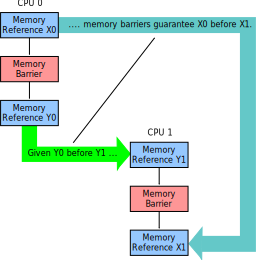
\includegraphics{memorder/memorybarrier}}
\caption{Memory Barriers Provide Conditional If-Then Ordering}
\label{fig:memorder:Memory Barriers Provide Conditional If-Then Ordering}
\end{figure}

\paragraph{Ordering has conditional if-then semantics.}
Figure~\ref{fig:memorder:Memory Barriers Provide Conditional If-Then Ordering}
는 메모리 배리어들을 위한 이 규칙을 보입니다.
두 메모리 배리어가 모두 충분히 강력하다 가정하고 (확신이 서지 않는다면, 언제든
\co{smp_mb()} 를 사용하세요), 만약 CPU~1 의 액세스 Y1 이 CPU~0 의 액세스 Y0
뒤에 일어났다면, CPU~1 의 액세스 X1 은 CPU~0 의 액세스 X1 뒤에 일어날 것이
보장됩니다.
\iffalse

Figure~\ref{fig:memorder:Memory Barriers Provide Conditional If-Then Ordering}
illustrates this for memory barriers.
Assuming that both memory barriers are strong enough (and when in doubt, you
can always use \co{smp_mb()}), if CPU~1's access Y1 happens after CPU~0's
access Y0, then CPU~1's access X1 is guaranteed to happen after CPU~0's
access X1.
\fi

\QuickQuiz{}
	특정 상황에서 어떤 메모리 배리어들이 충분히 강력한지 어떻게 이야기 할
	수 있나요?
	\iffalse

	How can you tell which memory barriers are strong enough for
	a given use case?
	\fi
\QuickQuizAnswer{
	아, 그건 답변하는데 이 챕터의 나머지 부분의 대부분을 필요로 할 만큼
	깊은 질문입니다.
	\iffalse

	Ah, that is a deep question whose answer requires most of the
	rest of this chapter.
	\fi
} \QuickQuizEnd

Listing~\ref{lst:memorder:Memory Ordering: Store-Buffering Litmus Test}
은 이 점에서의 한 예입니다.
Line~10 과~20 에서의 \co{smp_mb()} 는 배리어들의 역할을, line~9 에서의 \co{x0}
스토어는 X0 역할을, line~11 에서의 \co{x1} 으로부터의 로드는 Y0 를, line~19
에서의 \co{x1} 스토어는 Y1, 그리고 \co{x0} 로부터의 로드는 X1 역할을 합니다.
이 if-then 규칙을 단계별로 적용해 보면, 만약 \co{P0()} 의 로컬 변수 \co{r2} 가
값 0으로 설정되어 있다면 line~19 에서의 \co{x1} 스토어는 line~11 에서의 \co{x1}
로드 뒤에 일어났음을 알 수 있습니다.
그렇다면 이 if-then 규칙은 line~21 에서의 \co{x0} 으로부터의 로드가 line~9 의
\co{x0} 으로의 스토어 뒤에 일어났음을 이야기할 것입니다.
달리 말하자면,
\emph{만약} \co{P0()} 의 로컬 변수 \co{r2} 가 값 0으로 끝난다면 \co{P1()} 의
로컬 변수 \co{r2} 는 값 2로 끝날 것이 보장됩니다.
다시 말하지만, 메모리 순서 보장은 조건적이지, 절대적이지 않습니다.
\iffalse

Listing~\ref{lst:memorder:Memory Ordering: Store-Buffering Litmus Test}
is a case in point.
The \co{smp_mb()} on line~10 and~20 serve as the barriers,
the store to \co{x0} on line~9 as X0, the load from \co{x1} on line~11
as Y0, the store to \co{x1} on line~19 as Y1, and the load from
\co{x0} as X1.
Applying the if-then rule step by step, we know that the store to
\co{x1} on line~19 happens after the load from \co{x1} on line~11 if
\co{P0()}'s local variable \co{r2} is set to the value zero.
The if-then rule would then state that the load from \co{x0} on
line~21 happens after the store to \co{x0} on line~9.
In other words,
\co{P1()}'s local variable \co{r2} is guaranteed
to end up with the value two \emph{only if}
\co{P0()}'s local variable \co{r2} ends up with the value zero.
Again, memory ordering guarantees are conditional, not absolute.
\fi

비록
Figure~\ref{fig:memorder:Memory Barriers Provide Conditional If-Then Ordering}
가 구체적으로 메모리 배리어들을 언급하지만, 리눅스 커널의 나머지 순서 보장
오퍼레이셔들에도 같은 규칙이 적용됩니다.
\iffalse

Although
Figure~\ref{fig:memorder:Memory Barriers Provide Conditional If-Then Ordering}
specifically mentions memory barriers, the same rule applies to the
rest of the Linux kernel's ordering operations.
\fi

\paragraph{Ordering operations must be paired.}
여러분이 한 쓰레드에서의 오퍼레이션들의 순서는 주의깊게 맞췄지만, 다른
쓰레드에서는 그렇게 하는데 실패했다면, 순서가 없게 됩니다.
두 쓰레드 모두 앞의 if-then 규칙이 적용될 수 있도록 순서를 제공해야만
합니다.\footnote{
	Section~\ref{sec:memorder:Propagation} 에서, 짝 맞추기는 사이클로
	일반화 될겁니다.}
\iffalse

If you carefully order the operations in one thread, but then fail to do
so in another thread, then there is no ordering.
Both threads must provide ordering for the if-then rule to apply.\footnote{
	In Section~\ref{sec:memorder:Propagation}, pairing will be
	generalized to cycles.}
\fi

\paragraph{Ordering operations almost never speed things up.}
앞의 스토어가 메모리에 더 빨리 적용될 수 있도록 강제하기 위해 메모리 배리어를
추가하려 하고 있다면, 참으세요!
순서 보장을 추가하는건 일반적으로 일을 느려지게 만듭니다.
물론, 인스트럭션들을 추가하는 것이 일을 더 빨리 처리되게 만드는 경우도
있습니다만, 그런 경우에는 주의깊은 벤치마킹이 필요합니다.
그리고 설령 그렇다 하더라도, 여러분이 \emph{여러분의} 시스템에서 조금 속도를
높일 수 있었다 할지라도, 여러분의 사용자들의 시스템들에서는 상당히 속도가
떨어지는 경우가 있을 가능성도 있습니다.
또는 여러분의 미래의 시스템에서요.
\iffalse

If you find yourself tempted to add a memory barrier in an attempt
to force a prior store to be flushed to memory faster, resist!
Adding ordering usually slows things down.
Of course, there are situations where adding instructions speeds things
up, but careful benchmarking is required in such cases.
And even then, it is quite possible that although you sped things up
a little bit on \emph{your} system, you might well have slowed things
down significantly on your users' systems.
Or on your future system.
\fi

\paragraph{Ordering operations are not magic.}
여러분의 프로그램이 어떤 레이스 컨디션으로 문제가 발생한다면, 여러분의 버그가
존재하지 않도록 하기 위해 몇가지 메모리 순서 보장 오퍼레이션들을 추가하고
싶어지는 경우가 많을 겁니다.
이보다 훨씬 나은 반응은 주의깊게 설계된 형태로 더 높은 단계의 기능들을 사용하는
것입니다.
동시성 프로그래밍에서, 여러분의 버그들을 존재하지 않게 설계하는게 존재하지
않도록 꼼수를 부리는 것보다 거의 항상 쉽습니다!
\iffalse

When your program is failing due to some race condition, it is often
tempting to toss in a few memory-ordering operations in an attempt
to barrier your bug out of existence.
A far better reaction is to use higher-level primitives in a carefully
designed manner.
With concurrent programming, it is almost always easier to design
your bugs out of existence than to hack them out of existence!
\fi

\paragraph{These are only rough rules of thumb.}
비록 이 경험으로부터의 규칙들이 실제 현업에서 보여지는 대부분의 상황들을 다룰
수 있긴 하지만, 모든 경험으로부터의 규칙들이 그러하듯이 이 규칙들 역시 한계가
있습니다.
다음 섹션은 여러분의 직관을 깨부수고 여러분의 이해를 높여줄 trick-and-trap
리트머스 테스트들을 소개함으로써 이 한계들을 일부 보이겠습니다.
이 리트머시 테스트들은 또한
Table~\ref{tab:memorder:Linux-Kernel Memory-Ordering Cheat Sheet}
로 보여진 리눅스 커널 메모리 순셔규칙 커닝 페이퍼로 나타내어지는 개념들을
명확하게 할겁니다.
Section~\ref{sec:memorder:Where is Memory Ordering Needed?} 은 모든 트릭들과
함정들로부터 배운 것들을 가지고 이 커닝 페이퍼를 다시 한번 들여다 볼 겁니다.
\iffalse

Although these rules of thumb cover the vast majority of situations
seen in actual practice, as with any set of rules of thumb, they
do have their limits.
The next section will demonstrate some of these limits by introducing
trick-and-trap litmus tests that are intended to insult your
intuition while increasing your understanding.
These litmus tests will also illuminate many of the concepts
represented by the Linux-kernel memory-ordering cheat sheet shown in
Table~\ref{tab:memorder:Linux-Kernel Memory-Ordering Cheat Sheet}.
Section~\ref{sec:memorder:Where is Memory Ordering Needed?} will
circle back to this cheat sheet in light of learnings from all the
intervening tricks and traps.
\fi

\section{Tricks and Traps}
\label{sec:memorder:Tricks and Traps}

이제 하드웨어가 메모리 액세스 순서를 재배치 할 수 있고 여러분은 그걸 막을 수
있음을 알게 되었으니, 다음은 여러분이 여러분의 직관에 문제가 있음을 인정하도록
할 차례입니다.
이 고통스러운 작업은 scalar 변수들이 동시에 여러 값들을 가지고 있음을 보이는
코드를 소개하는
Section~\ref{sec:memorder:Variables With Multiple Values}, 그리고
직관적으로 올바르지만 실제 하드웨어에서는 비참하게 실패하고 마는 코드들을
보이는
Sections~\ref{sec:memorder:Memory-Reference Reordering} 부터
\ref{sec:memorder:Multicopy Atomicity} 까지를 통해 이루어질 겁니다.
이 비탄의 작업을 통해 일단 여러분의 직관이 만들어지면, 뒤의 섹션들에서 우리가
근간으로 삼게 될, 메모리 배리어들이 따르는 기본 규칙들을 제공합니다.
이 규칙들은 더 나아가

하지만 먼저, 한 순간에 하나의 변수가 얼마나 많은 값들을 가지고 있을 수 있는지
간단히 알아봅시다.
\iffalse

Now that you know that hardware can reorder memory accesses and that you
can prevent it from doing so, the next step is to get you to admit
that your intuition has a problem.
This painful task is taken up by
Section~\ref{sec:memorder:Variables With Multiple Values},
which presents some code demonstrating that scalar variables can
take on multiple values simultaneously,
and by
Sections~\ref{sec:memorder:Memory-Reference Reordering} through
\ref{sec:memorder:Multicopy Atomicity},
which show a series of intuitively correct code fragments that fail miserably
on real hardware.
Once your intuition has made it through the grieving process, later
sections will summarize the basic rules that memory ordering follows.

But first, let's take a quick look at just how many values a single
variable might have at a single moment of time.
\fi

\subsection{Variables With Multiple Values}
\label{sec:memorder:Variables With Multiple Values}

하나의 변수는 잘 정의된 전역적 순서로 값들의 연속을 갖게 될 거라 생각하는건
자연스럽습니다.
불행히도, 이 여정의 다음 정류장은 이 편안한 거짓에 ``작별''을 고하라 합니다.
바라건대, 여러분은 이미
Tables~\ref{tab:memorder:Memory Misordering: Store-Buffering Sequence of Events}
와~\ref{tab:memorder:Memory Ordering: Store-Buffering Sequence of Events} 의
row~2 를 통해 ``작별'' 을 고하기 시작했을 것이고 만약 그렇다면 이 섹션의 목적은
이 요점을 제대로 이끌어내는 것입니다.
\iffalse

It is natural to think of a variable as taking on a well-defined
sequence of values in a well-defined, global order.
Unfortunately, the next stop on the journey says ``goodbye'' to this comforting fiction.
Hopefully, you already started to say ``goodbye'' in response to row~2 of
Tables~\ref{tab:memorder:Memory Misordering: Store-Buffering Sequence of Events}
and~\ref{tab:memorder:Memory Ordering: Store-Buffering Sequence of Events},
and if so, the purpose of this section is to drive this point home.
\fi

그러기 위해,
Listing~\ref{lst:memorder:Software Logic Analyzer} 에 보인 프로그램의 한 부분을
고려해 봅시다.
이 코드 조각은 여러 CPU 들에서 병렬적으로 수행됩니다.
Line~1 은 하나의 공유 변수를 현재 CPU 의 ID 로 값을 할당하고, line~2 에서는
모든 CPU 들 가운데 동기화 되는 (불행히도, 모든 CPU 구조에서 가능한 일은
아닙니다!) 하드웨어 ``timebase'' 카운터의 값을 가져오는 \co{gettb()} 함수를
사용해 일부 변수들을 초기화 시키고, line~3-8 의 루프에서는 이 CPU 가 할당한
값이 유지된 시간의 길이를 기록합니다.
물론, 이 CPU 들 가운데 하나는 ``승리'' 할 것이고, 따라서 line~6-7 의 검사가
아니라면 이 루프를 절대 빠져나오지 않을 겁니다.
\iffalse

To this end, consider the program fragment shown in
Listing~\ref{lst:memorder:Software Logic Analyzer}.
This code fragment is executed in parallel by several CPUs.
Line~1 sets a shared variable to the current CPU's ID, line~2
initializes several variables from a \co{gettb()} function that
delivers the value of a fine-grained hardware ``timebase'' counter that is
synchronized among all CPUs (not available from all CPU architectures,
unfortunately!), and the loop from lines~3-8 records the length of
time that the variable retains the value that this CPU assigned to it.
Of course, one of the CPUs will ``win'', and would thus never exit
the loop if not for the check on lines~6-7.
\fi

\QuickQuiz{}
	Listing~\ref{lst:memorder:Software Logic Analyzer}
	의 코드에서의 어떤 가정이 실제 하드웨어에서는 성립하지 않을까요?
	\iffalse

	What assumption is the code fragment
	in Listing~\ref{lst:memorder:Software Logic Analyzer}
	making that might not be valid on real hardware?
	\fi
\QuickQuizAnswer{
	이 코드는 특정 CPU 가 자신의 값을 보는 것을 멈추자마자, 곧바로
	마지막으로 동의된 값을 보게 될 것이라 가정삽니다.
	실제 하드웨어에서, 어떤 CPU 들은 이 마지막 값을 보게 되기 전에 중간의
	결과를 일부 보게 될수도 있습니다.
	따라서 이 섹션의 뒤에서 이야기될 그림들의 데이터를 만드는데 사용된 실제
	코드는 좀 더 복잡합니다.
	\iffalse

	The code assumes that as soon as a given CPU stops
	seeing its own value, it will immediately see the
	final agreed-upon value.
	On real hardware, some of the CPUs might well see several
	intermediate results before converging on the final value.
	The actual code used to produce the data in the figures
	discussed later in this section was therefore somewhat more
	complex.
	\fi
} \QuickQuizEnd

\begin{listing}[tbp]
{ \scriptsize
\begin{verbbox}
  1 state.variable = mycpu;
  2 lasttb = oldtb = firsttb = gettb();
  3 while (state.variable == mycpu) {
  4   lasttb = oldtb;
  5   oldtb = gettb();
  6   if (lasttb - firsttb > 1000)
  7     break;
  8 }
\end{verbbox}
}
\centering
\theverbbox
\caption{Software Logic Analyzer}
\label{lst:memorder:Software Logic Analyzer}
\end{listing}

루프를 빠져나오기 전, \co{firsttb} 는 앞의 공유 변수에의 값 할당 후 곧바로
가져온 timestamp 를 가지고 있을 것이고 \co{lasttb} 는 여전히 할당된 값을 가지고
있을, 이 공유 변수의 마지막 샘플링 전에 가져온 timestamp 를 가지고 있을 수도
있고, 만약 이 공유 변수가 루프에 들어오기 전에 바뀌었다면 \co{firsttb} 와 같은
값을 가지고 있을 수도 있습니다.
이는 우리가 532-나노세컨드의 시간 간격 동안의 각 CPU 의 \co{state.variable} 의
값에 대한 관찰을 그려볼 수 있게 해주는데,
Figure~\ref{fig:memorder:A Variable With Multiple Simultaneous Values} 에
보여져 있습니다.
이 데이터는 2006년에 각각 두개의 하드웨어 쓰레드를 갖는 8개의 코어를 장착한
1.5\,GHz POWER5 시스템에서 수집되었습니다.
CPU~1, 2, 3, 그리고~4 는 이 값들을 기록했고, CPU~0 는 이 테스트를 제어했습니다.
Timebase 카운터의 시간 간격은 5.32\,ns 정도였는데, 이는 중간의 캐시 상태들을
관찰하기에 충분히 작은 간격입니다.
\iffalse

Upon exit from the loop, \co{firsttb} will hold a timestamp
taken shortly after the assignment and \co{lasttb} will hold
a timestamp taken before the last sampling of the shared variable
that still retained the assigned value, or a value equal to \co{firsttb}
if the shared variable had changed before entry into the loop.
This allows us to plot each CPU's view of the value of \co{state.variable}
over a 532-nanosecond time period, as shown in
Figure~\ref{fig:memorder:A Variable With Multiple Simultaneous Values}.
This data was collected in 2006 on 1.5\,GHz POWER5 system with 8 cores,
each containing a pair of hardware threads.
CPUs~1, 2, 3, and~4 recorded the values, while CPU~0 controlled the test.
The timebase counter period was about 5.32\,ns, sufficiently fine-grained
to allow observations of intermediate cache states.
\fi

\begin{figure}[htb]
\centering
\resizebox{3in}{!}{\includegraphics{memorder/MoreThanOneValue}}
\caption{A Variable With Multiple Simultaneous Values}
\label{fig:memorder:A Variable With Multiple Simultaneous Values}
\end{figure}

각각의 수평의 막대는 해당 CPU 의 관찰 결과를 시간대별로 보여주는데, 왼쪽 검은
영역은 해당 CPU 의 첫번째 관측 전까지의 시간을 나타냅니다.
처음 5\,ns 동안, CPU~3 만이 이 변수의 값을 읽었습니다.
그 다음 10\,ns 동안, CPU~2 와~3 은 이 변수의 값을 서로 다르게 이야기했는데, 그
후에는 최종적으로 동의된 값인 ``2'' 라는 값에 합의했습니다.
하지만, CPU~1 은 이 값이 ``1'' 이라고 거의 300\,ns 동안 믿었고, CPU~4 는 거의
500\,ns 동안이나 이 값이 ``4'' 라고 믿었습니다.
\iffalse

Each horizontal bar represents the observations of a given CPU over time,
with the black regions to the left indicating the time before the
corresponding CPU's first measurement.
During the first 5\,ns, only CPU~3 has an opinion about the value of the
variable.
During the next 10\,ns, CPUs~2 and~3 disagree on the value of the variable,
but thereafter agree that the value is~``2'', which is in fact
the final agreed-upon value.
However, CPU~1 believes that the value is~``1'' for almost 300\,ns, and
CPU~4 believes that the value is~``4'' for almost 500\,ns.
\fi

\QuickQuiz{}
	어떻게 CPU 들이 하나의 변수를 \emph{동시에} 서로 다르게 볼 수가
	있는거죠?
	\iffalse

	How could CPUs possibly have different views of the
	value of a single variable \emph{at the same time?}
	\fi
\QuickQuizAnswer{
	Section~\ref{sec:memorder:Why Hardware Misordering?}
	에서 논의된 대로, 많은 CPU 들이 최근의 스토어 값을 기록하는 스토어
	버퍼를 가지고 있으며, 이 값은 연관된 캐시 라인이 해당 CPU 로 올라오기
	전에는 외부에 보여지지 않습니다.
	따라서, 각 CPU 가 하나의 시점에 특정 변수에 대해 서로 다른 값을 보고
	있는 것이---그리고 메인 메모리는 또 다른 값을 가지고 있는 것이
	가능합니다.
	메모리 배리어가 발명된 이유들 중 하나는 소프트웨어가 이런 종류의 상황을
	우아하게 처리할 수 있도록 해주기 위함이었습니다.
	\iffalse

	As discussed in
	Section~\ref{sec:memorder:Why Hardware Misordering?},
	many CPUs have store buffers that record the values of
	recent stores, which do not become globally visible until
	the corresponding cache line makes its way to the CPU.
	Therefore, it is quite possible for each CPU to see a
	different value for a given variable at a single point
	in time---and for main memory to hold yet another value.
	One of the reasons that memory barriers were invented was
	to allow software to deal gracefully with situations like
	this one.
	\fi
} \QuickQuizEnd

\QuickQuiz{}
	CPU~1 과~4 는 값을 동의하는데에 그렇게 오랜 시간이 걸렸는데, CPU~2 와~3
	은 어떻게 그렇게 빨리 값에 동의하는 건가요?
	\iffalse

	Why do CPUs~2 and~3 come to agreement so quickly, when it
	takes so long for CPUs~1 and~4 to come to the party?
	\fi
\QuickQuizAnswer{
	CPU~2 와~3 은 같은 코어의 하드웨어 쓰레드들이어서 같은 캐시 계층을
	공유하며, 따라서 매우 낮은 통신 응답시간을 갖습니다.
	이게 NUMA, 또는, 보다 정확히는, NUCA 효과입니다.

	이는 CPU~2 와~3 가 왜 값에 대해 동의하지 않는 순간이 존재하긴 하는가에
	대한 질문을 떠올리게 합니다.
	가능한 한가지 이유는 이들이 커다란 공유된 캐시 외에 작은 개별 캐시를
	갖고 있을 수 있다는 것입니다.
	여기서의 짧은 10-나노세컨드 동안의 비동의된 시간과 해당 코드에 메모리
	배리어가 아예 없었다는 것을 놓고 보면, 또다른 가능할 법한 이유는
	인스트럭션 재배치입니다.
	\iffalse

	CPUs~2 and~3 are a pair of hardware threads on the same
	core, sharing the same cache hierarchy, and therefore have
	very low communications latencies.
	This is a NUMA, or, more accurately, a NUCA effect.

	This leads to the question of why CPUs~2 and~3 ever disagree
	at all.
	One possible reason is that they each might have a small amount
	of private cache in addition to a larger shared cache.
	Another possible reason is instruction reordering, given the
	short 10-nanosecond duration of the disagreement and the
	total lack of memory barriers in the code fragment.
	\fi
} \QuickQuizEnd

그리고 네개의 CPU 에서의 상황이 재밌다고 생각한다면, 같은 상황을 15~CPU 들이
각각 시간 $t=0$ 에 하나의 공유 변수에 각자의 숫자를 할당하는 경우를 보인
Figure~\ref{fig:memorder:A Variable With More Simultaneous Values} 를 고려해
보세요.
해당 그림의 두 다이어그램은 모두
Figure~\ref{fig:memorder:A Variable With Multiple Simultaneous Values} 와 같은
방식으로 그려졌습니다.
유일한 차이점은 가로축의 단위가 timebase tick 으로, 각 tick 은 약
5.3~나노세컨드를 의미합니다.
따라서 여기서의 전체 연속된 값의 변화는 CPU 의 수의 증가에 일관되게
Figure~\ref{fig:memorder:A Variable With Multiple Simultaneous Values} 에서보다
긴 시간동안 유지되었습니다.
위의 다이어그램은 전체 그림을 보이며, 아래쪽의 것은 첫 50~timebase tick 만을
확대해서 보입니다.

여기서도, CPU~0 는 테스트를 제어했고, 따라서 어떤 값도 기록하지 않았습니다.
\iffalse

And if you think that the situation with four CPUs was intriguing, consider
Figure~\ref{fig:memorder:A Variable With More Simultaneous Values},
which shows the same situation, but with 15~CPUs each assigning their
number to a single shared variable at time~$t=0$. Both diagrams in the
figure are drawn in the same way as 
Figure~\ref{fig:memorder:A Variable With Multiple Simultaneous Values}.
The only difference is that the unit of horizontal axis is timebase ticks,
with each tick lasting about 5.3~nanoseconds.
The entire sequence therefore lasts a bit longer than the events recorded in
Figure~\ref{fig:memorder:A Variable With Multiple Simultaneous Values},
consistent with the increase in number of CPUs.
The upper diagram shows the overall picture, while the lower one shows
the zoom-up of first 50~timebase ticks.

Again, CPU~0 coordinates the test, so does not record any values.
\fi

\begin{figure*}
\centering
\resizebox{5in}{!}{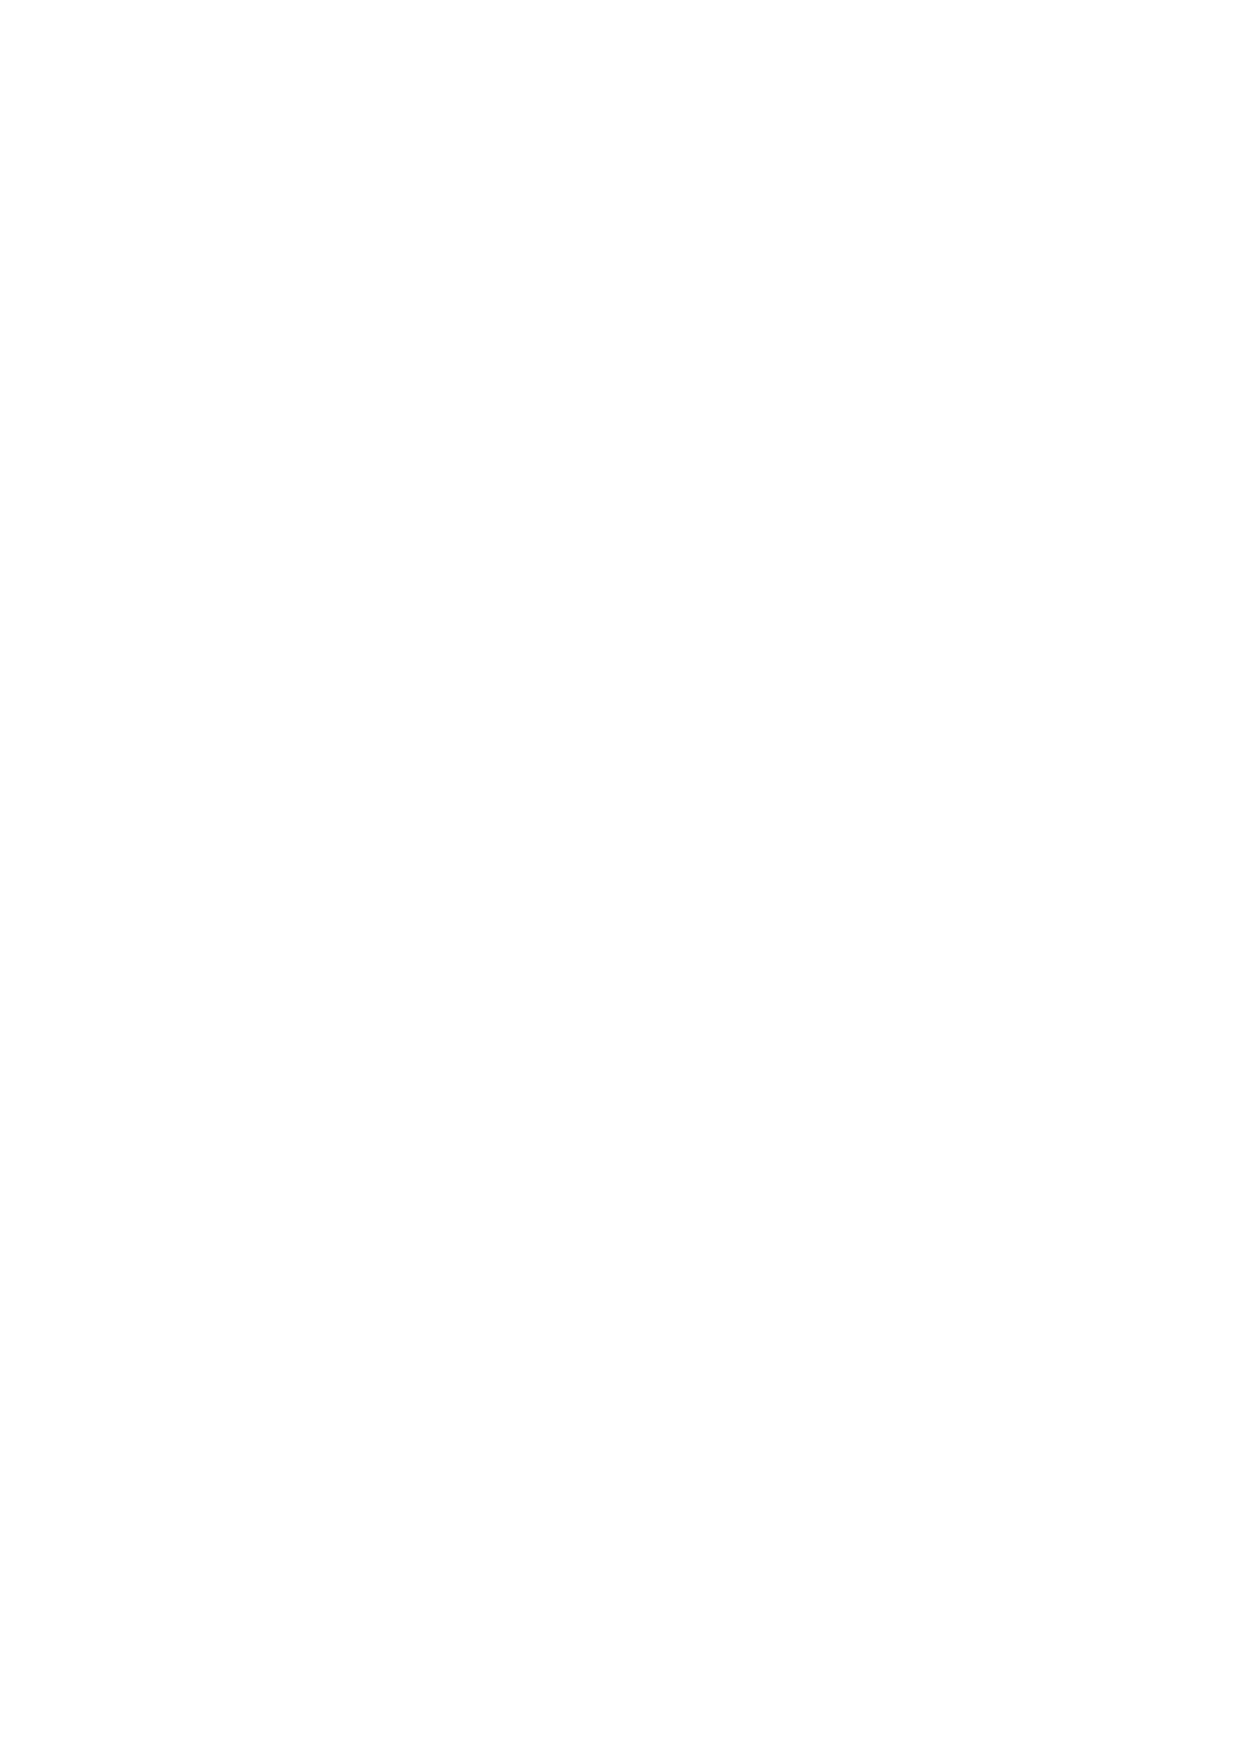
\includegraphics{memorder/MoreThanOneValue-15CPU}}
\caption{A Variable With More Simultaneous Values}
\ContributedBy{Figure}{fig:memorder:A Variable With More Simultaneous Values}{Akira Yokosawa}
\end{figure*}

모든 CPU 들이 결국은 마지막 값~9 에 동의를 합니다만, 값~15 와 값~12 가 먼저
상황을 이끈 후입니다.
아래쪽 다이어그램의 수직선으로 나타내어진 time~21 시점에 변수의 값에 대한
14개의 서로 다른 의견들이 존재했음을 알아두시기 바랍니다.
또한 모든 CPU 들이 값들의 순서에 대해
Figure~\ref{fig:memorder:Possible Global Orders With More Simultaneous Values}
에 보인 방향성 있는 그래프의 순서와 일관된 순서를 보았음을 알아두시기 바랍니다.
더도 아니고 덜도 아니고, 두 그림은 메모리 접근 순서에 신경 쓰는 코드에서의
메모리 배리어의 올바른 사용의 중요성을 강조합니다.
\iffalse

All CPUs eventually agree on the final value of~9, but not before
the values~15 and~12 take early leads.
Note that there are fourteen different opinions on the variable's value
at time~21 indicated by the vertical line in the lower diagram.
Note also that all CPUs see sequences whose orderings are consistent with
the directed graph shown in
Figure~\ref{fig:memorder:Possible Global Orders With More Simultaneous Values}.
Nevertheless, both figures underscore the importance of
proper use of memory barriers for code that cares about memory ordering.
\fi

\begin{figure}[htb]
\centering
\resizebox{2.0in}{!}{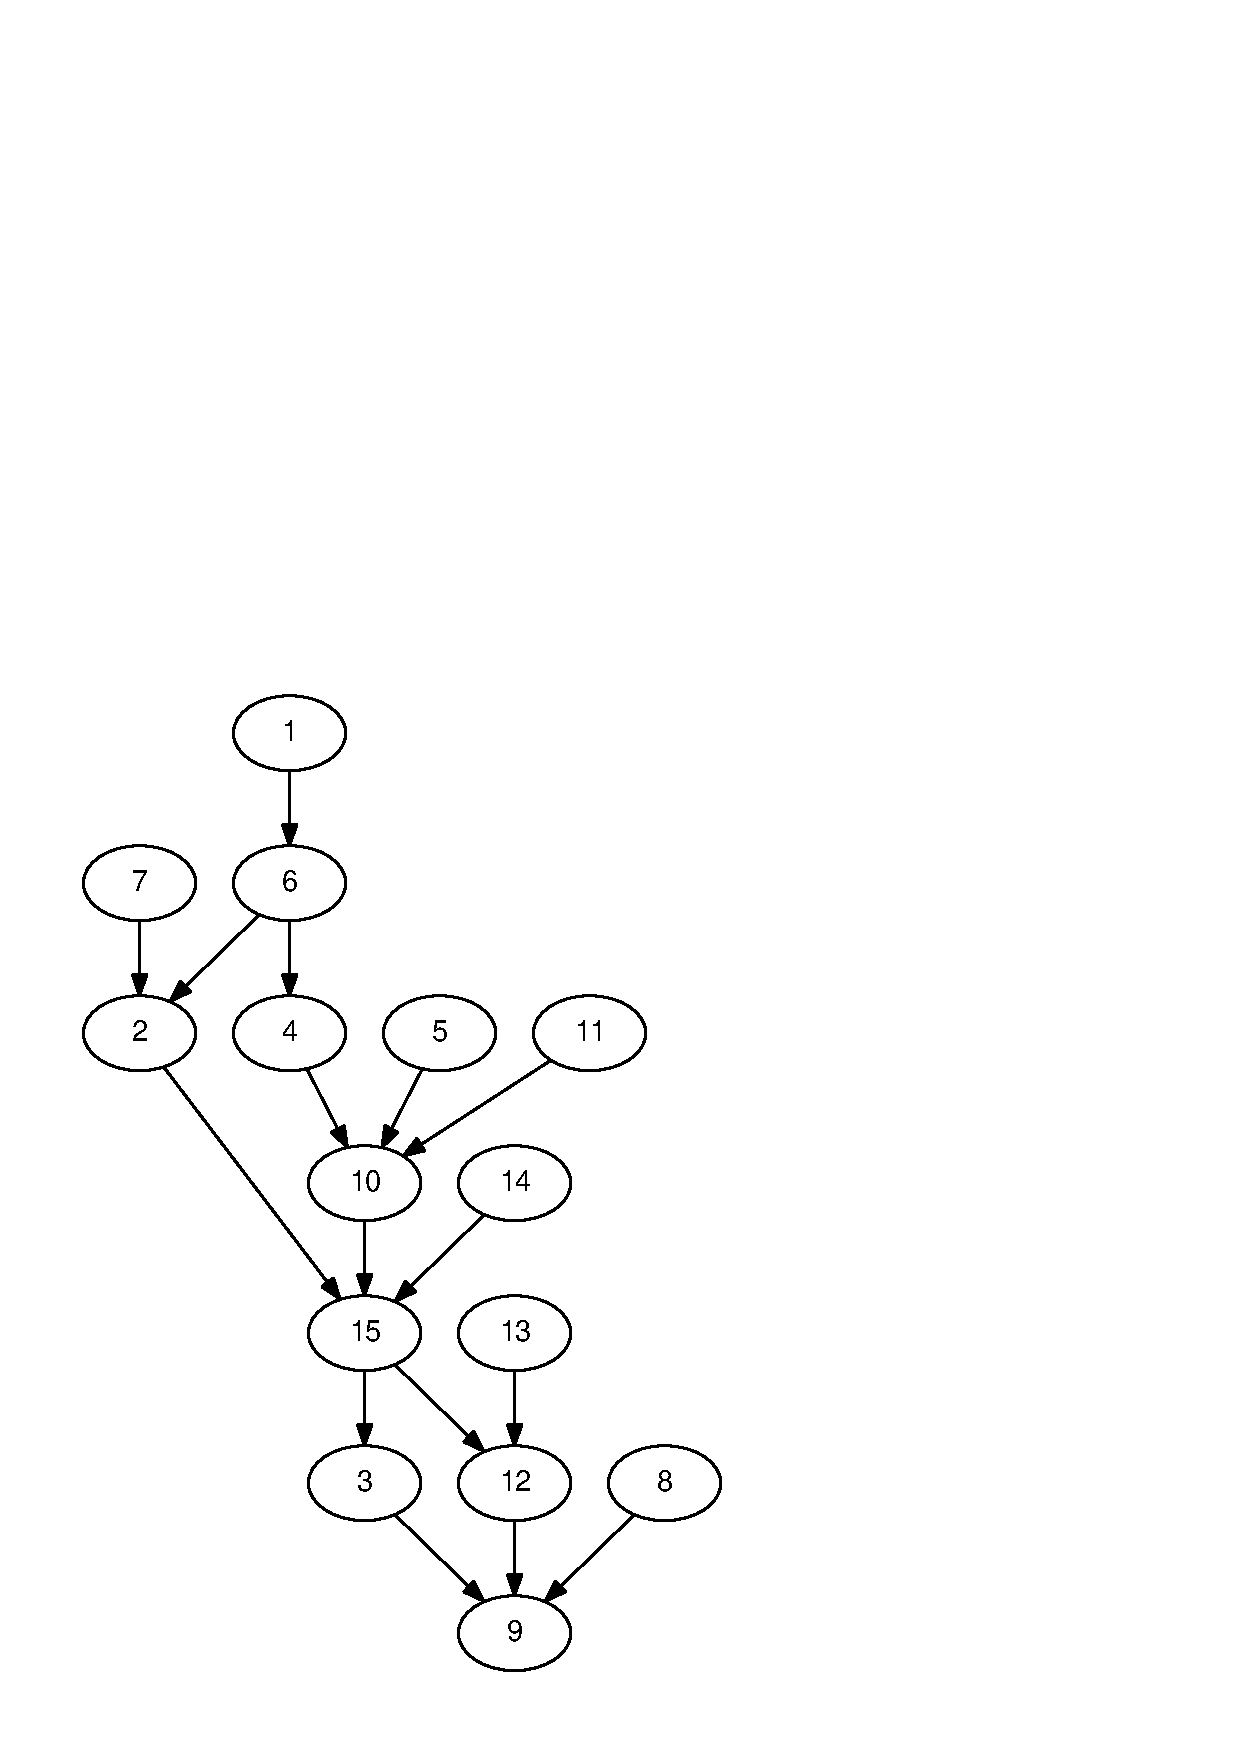
\includegraphics{memorder/store15tred}}
\caption{Possible Global Orders With More Simultaneous Values}
\label{fig:memorder:Possible Global Orders With More Simultaneous Values}
\end{figure}

하나의 변수는 한 시점에 얼마나 많은 값들을 가질 수 있을까요?
시스템에 존재하는 스토어 버퍼 하나당 하나씩입니다!
따라서 우리는 변수들의 값들과 시간의 흐름에 대한 편안한 직관에게 작별을
고해야만 하는 체제에 들어섰습니다.
이는 메모리 배리어들이 필요한 체제입니다.

이와 함께,
Chapter~\ref{chp:Hardware and its Habits}
와~\ref{cha:Partitioning and Synchronization Design} 에서 배웠던 교훈들을
기억할 필요가 있습니다.
모든 CPU 들이 같은 변수에게 동시에 스토어를 하도록 하는 것은 병렬 프로그램을
설계하는 방법이 아닌데, 적어도 성능과 확장성이 여러분에게 전혀 중요하지 않은 게
아니라면 그렇습니다.

불행히도, 메모리 순서 규칙은 여러분의 직관을 망칠 수 있는 방법들을 이외에도
많이 가지고 있으며, 이런 방법들 모두가 성능과 확장성을 훼손하는 건 아닙니다.
다음 섹션은 관계없는 메모리 참조의 순서 재배치에 대한 소개를 제공합니다.
\iffalse

How many values can a single variable take on at a single point in
time?
As many as one per store buffer in the system!
We have therefore entered a regime where we must bid a fond farewell to
comfortable intuitions about values of variables and the passage of time.
This is the regime where memory barriers are needed.

All that aside, it is important to remember the lessons from
Chapters~\ref{chp:Hardware and its Habits}
and~\ref{cha:Partitioning and Synchronization Design}.
Having all CPUs store concurrently to the same variable
is absolutely no way to design a parallel program, at least
not if performance and scalability are at all important to you.

Unfortunately, memory ordering has many other ways of insulting your
intuition, and not all of these ways conflict with performance and
scalability.
The next section will give an overview of reordering of unrelated
memory reference.
\fi

\subsection{Memory-Reference Reordering}
\label{sec:memorder:Memory-Reference Reordering}

Section~\ref{sec:memorder:Why Hardware Misordering?}
에서는 x86 과 같이 상대적으로 강력한 순서 규칙의 시스템들도 앞의 스토어들을
뒤의 로드들과 만약 이 스토어와 로드가 서로 다른 변수들에 대해 행해진다면 재배치
시킬 수 있다는 것을 보였습니다.
이 섹션은 이 결과에 기반해서, 다른 로드와 스토어 조합을 봅니다.
\iffalse

Section~\ref{sec:memorder:Why Hardware Misordering?}
showed that even relatively strongly ordered systems like x86
can reorder prior stores with later loads, at least when the
store and load are to different variables.
This section builds on that result, looking at the other combinations of
loads and stores.
\fi

% @@@ Rationale for further reordering.

\begin{listing}[tbp]
{ \scriptsize
\begin{verbbox}[\LstLineNo]
C C-MP+o-wmb-o+o-o

{
}


P0(int* x0, int* x1) {

  WRITE_ONCE(*x0, 2);
  smp_wmb();
  WRITE_ONCE(*x1, 2);

}

P1(int* x0, int* x1) {

  int r2;
  int r3;

  r2 = READ_ONCE(*x1);
  r3 = READ_ONCE(*x0);

}

exists (1:r2=2 /\ 1:r3=0)
\end{verbbox}
}
\centering
\theverbbox
\caption{Message-Passing Litmus Test (No Ordering)}
\label{lst:memorder:Message-Passing Litmus Test (No Ordering)}
\end{listing}

\subsubsection{Load Followed By Load}
Listing~\ref{lst:memorder:Message-Passing Litmus Test (No Ordering)}
(\path{C-MP+o-wmb-o+o-o.litmus})
는 고전적 \emph{message-passing} 리트머스 테스트를 보이는데, 여기서 \co{x0} 는
메세지이고 \co{x1} 은 메세지가 존재하는지 여부를 알리는 플래그입니다.
이 테스트에서, \co{smp_wmb()} 는 \co{P0()} 의 스토어들이 순서대로 행해지게
강제하지만, 로드들에 대해서는 어떤 순서도 강제하지 않습니다.
x86 과 같이 상대적으로 강력한 순서 규칙의 아키텍쳐들에서는 순서를 강제합니다.
하지만, 완화된 순서 규칙의 아키텍쳐들은 그렇지 않은 경우가
많습니다~\cite{JadeAlglave2011ppcmem}.
따라서, 이 listing 의 line~25 에서의 \co{exists} 절은 발동될 수
\emph{있습니다}.
\iffalse

Listing~\ref{lst:memorder:Message-Passing Litmus Test (No Ordering)}
(\path{C-MP+o-wmb-o+o-o.litmus})
shows the classic \emph{message-passing} litmus test, where \co{x0} is
the message and \co{x1} is a flag indicating whether or not a message
is available.
In this test, the \co{smp_wmb()} forces \co{P0()} stores to be ordered,
but no ordering is specified for the loads.
Relatively strongly ordered architectures, such as x86, do enforce ordering.
However, weakly ordered architectures often do
not~\cite{JadeAlglave2011ppcmem}.
Therefore, the \co{exists} clause on line~25 of the listing \emph{can}
trigger.
\fi

\begin{listing}[tbp]
{ \scriptsize
\begin{verbbox}[\LstLineNo]
C C-MP+o-wmb-o+o-rmb-o

{
}

P0(int* x0, int* x1) {

  WRITE_ONCE(*x0, 2);
  smp_wmb();
  WRITE_ONCE(*x1, 2);

}

P1(int* x0, int* x1) {

  int r2;
  int r3;

  r2 = READ_ONCE(*x1);
  smp_rmb();
  r3 = READ_ONCE(*x0);

}

exists (1:r2=2 /\ 1:r3=0)
\end{verbbox}
}
\centering
\theverbbox
\caption{Enforcing Order of Message-Passing Litmus Test}
\label{lst:memorder:Enforcing Order of Message-Passing Litmus Test}
\end{listing}

따라서, 이 경우에 순서에 의존적이고 완화된 순서규칙의 아키텍쳐에도 이식될 수
있을 법한 코드에서는 명시적인 순서 규칙을 추가해야 하는데, 예를 들면
Listing~\ref{lst:memorder:Enforcing Order of Message-Passing Litmus Test}
(\path{C-MP+o-wmb-o+o-rmb-o.litmus})
의 line~20 에 보인, \co{exists} 절이 발동될 수 없게 하는 \co{smp_rmb()} 를
추가하는 식입니다.
\iffalse

Thus, portable code relying on ordering in this case must
add explicit ordering, for example, the \co{smp_rmb()} shown on
line~20 of
Listing~\ref{lst:memorder:Enforcing Order of Message-Passing Litmus Test}
(\path{C-MP+o-wmb-o+o-rmb-o.litmus}), which prevents
the \co{exists} clause from triggering.
\fi

\begin{listing}[tbp]
{ \scriptsize
\begin{verbbox}[\LstLineNo]
C C-LB+o-o+o-o
{
}

P0(int *x0, int *x1)
{
  int r2;

  r2 = READ_ONCE(*x1);
  WRITE_ONCE(*x0, 2);
}


P1(int *x0, int *x1)
{
  int r2;

  r2 = READ_ONCE(*x0);
  WRITE_ONCE(*x1, 2);
}

exists (1:r2=2 /\ 0:r2=2)
\end{verbbox}
}
\centering
\theverbbox
\caption{Load-Buffering Litmus Test (No Ordering)}
\label{lst:memorder:Load-Buffering Litmus Test (No Ordering)}
\end{listing}

\subsubsection{Load Followed By Store}
Listing~\ref{lst:memorder:Load-Buffering Litmus Test (No Ordering)}
(\path{C-LB+o-o+o-o.litmus})
은 고전적인 \emph{load-buffering} 리트머스 테스트를 보입니다.
x86 이나 IBM Mainframe 과 같이 비교적 강력한 순서규칙을 가진 시스템들은 앞의
로드들을 뒤따르는 스토어들과 재배치 하지 않지만, 더 완화된 순서 규칙의
아키텍쳐들은 그런 재배치를 정말로 허용합니다~\cite{JadeAlglave2011ppcmem}.
따라서, line~22 의 \co{exists} 절은 정말로 발동될 수 있습니다.
\iffalse

Listing~\ref{lst:memorder:Load-Buffering Litmus Test (No Ordering)}
(\path{C-LB+o-o+o-o.litmus})
shows the classic \emph{load-buffering} litmus test.
Although relatively strongly ordered systems such as x86
or the IBM Mainframe do not reorder prior loads with subsequent stores,
more weakly ordered architectures really do allow such
reordering~\cite{JadeAlglave2011ppcmem}.
Therefore, the \co{exists} clause on line~22 really can trigger.
\fi

\begin{listing}[tbp]
{ \scriptsize
\begin{verbbox}[\LstLineNo]
C C-LB+o-r+a-o
{
}

P0(int *x0, int *x1)
{
  int r2;

  r2 = READ_ONCE(*x1);
  smp_store_release(x0, 2);
}


P1(int *x0, int *x1)
{
  int r2;

  r2 = smp_load_acquire(x0);
  WRITE_ONCE(*x1, 2);
}

exists (1:r2=2 /\ 0:r2=2)
\end{verbbox}
}
\centering
\theverbbox
\caption{Enforcing Ordering of Load-Buffering Litmus Test}
\label{lst:memorder:Enforcing Ordering of Load-Buffering Litmus Test}
\end{listing}

실제 하드웨어가 이런 재배치를 하는건 비교적 드문
일이긴 합니다만~\cite{LucMaranget2017aarch64},
이식성 있는 코드는 더도 말고 덜도 말고
Listing~\ref{lst:memorder:Enforcing Ordering of Load-Buffering Litmus Test}
(\path{C-LB+o-r+a-o.litmus})
에 보인 것과 같이 모든 필요한 순서 규칙을 강제해야만 합니다.
이는 line~22 의 \co{exists} 절이 절대 발동되지 않을 것을 보장합니다.
\iffalse

Although it is rare for actual hardware to
exhibit this reordering~\cite{LucMaranget2017aarch64},
portable code must nevertheless enforce any required ordering, for example,
as shown in
Listing~\ref{lst:memorder:Enforcing Ordering of Load-Buffering Litmus Test}
(\path{C-LB+o-r+a-o.litmus}).
This guarantees that the \co{exists} clause on line~22 never triggers.
\fi

\begin{listing}[tbp]
{ \scriptsize
\begin{verbbox}[\LstLineNo]
C C-MP+o-o+o-rmb-o

{
}

P0(int* x0, int* x1) {

  WRITE_ONCE(*x0, 2);
  WRITE_ONCE(*x1, 2);

}

P1(int* x0, int* x1) {

  int r2;
  int r3;

  r2 = READ_ONCE(*x1);
  smp_rmb();
  r3 = READ_ONCE(*x0);

}

exists (1:r2=2 /\ 1:r3=0)
\end{verbbox}
}
\centering
\theverbbox
\caption{Message-Passing Litmus Test, No Writer Ordering (No Ordering)}
\label{lst:memorder:Message-Passing Litmus Test, No Writer Ordering (No Ordering)}
\end{listing}

\subsubsection{Store Followed By Store}
Listing~\ref{lst:memorder:Message-Passing Litmus Test, No Writer Ordering (No Ordering)}
(\path{C-MP+o-o+o-rmb-o.litmus})
은 다시 한번 고전적 메세지 패싱 리트머스 테스트를 보이는데, 이번에는 \co{P0()}
로의 스토어들에 대한 명시적 순서가 없고 \co{P1()} 의 로드들에 대한 순서가
\co{smp_rmb()} 로 제공되어진 버전입니다.
다시 한번 말하지만, 상대적으로 강력한 순서 규칙의 아키텍쳐들은 순서를
지켜주지만, 완화된 순서 규칙의 아키텍쳐들은 그러지 않기
때문에~\cite{JadeAlglave2011ppcmem}, \co{exists} 절은 발동될 수 있습니다.
따라서, 이식성 있는 코드는
Listing~\ref{lst:memorder:Enforcing Order of Message-Passing Litmus Test} 에서
보인 것과 같이 스토어들에도 명시적 순서를 부여해서 \co{exists} 절이 발동되지
않게 해야만 합니다.
\iffalse

Listing~\ref{lst:memorder:Message-Passing Litmus Test, No Writer Ordering (No Ordering)}
(\path{C-MP+o-o+o-rmb-o.litmus})
once again shows the classic message-passing litmus test, but without
explicit ordering for \co{P0()}'s stores and with the \co{smp_rmb()}
providing ordering for \co{P1()}'s loads.
Again, the relatively strongly ordered architectures do enforce ordering,
but weakly ordered architectures do not necessarily do
so~\cite{JadeAlglave2011ppcmem}, which means that the
\co{exists} clause can trigger.
Therefore, portable code must explicitly order the stores, for
example, as shown in
Listing~\ref{lst:memorder:Enforcing Order of Message-Passing Litmus Test},
thus preventing the \co{exists} clause from triggering.
\fi

\subsection{Address Dependencies}
\label{sec:memorder:Address Dependencies}

\emph{Address dependency} 는 로드 인스트럭션에 의해 리턴된 값이 나중의 메모리
레퍼런스 인스트럭션에 의해 사용되는 주소의 계산에 사용될 때 발생합니다.
\iffalse

An \emph{address dependency} occurs when the value returned by a load
instruction is used to compute the address used by a later memory-reference
instruction.
\fi

\begin{listing}[tbp]
{ \scriptsize
\begin{verbbox}[\LstLineNo]
C C-MP+o-wmb-o+o-addr-o

{
int y=1;
int *x1 = &y;
}

P0(int* x0, int** x1) {

  WRITE_ONCE(*x0, 2);
  smp_wmb();
  WRITE_ONCE(*x1, x0);

}

P1(int** x1) {

  int *r2;
  int r3;

  r2 = READ_ONCE(*x1);
  r3 = READ_ONCE(*r2);

}

exists (1:r2=x0 /\ 1:r3=1)
\end{verbbox}
}
\centering
\theverbbox
\caption{Message-Passing Address-Dependency Litmus Test (No Ordering)}
\label{lst:memorder:Message-Passing Address-Dependency Litmus Test (No Ordering)}
\end{listing}

Listing~\ref{lst:memorder:Message-Passing Address-Dependency Litmus Test (No Ordering)}
(\path{C-MP+o-wmb-o+o-addr-o.litmus})
은 message-passing 패턴의 링크 버전을 보입니다.
헤드 포인터는 \co{x1} 으로, 최초에 \co{int} 변수 \co{y} 를 가리키게 되며
(line~5), 변수 \co{y} 는 초기값 $1$ 을 갖습니다 (line~4).
\co{P0()} 는 헤드 포인터 \co{x1} 이 \co{x0} 를 가리키도록 업데이트 (line~12)
하는데 이는 \co{x0} 가 $2$ 로 초기화 (line~10) 된 후로 순서지어집니다
(line~11).
\co{P1()} 은 헤드 포인터 \co{x1} 을 가져오고 (line~21) 이를 통해 레퍼런스되는
값을 가져옵니다 (line~22).
따라서 line~21 의 로드와 line~22 의 로드 사이에는 address dependency 가
존재합니다.
이 경우에, line~21 에서 리턴되는 값은 line~22 에서 사용되는 주소값 그
자체이지만, C-언어의 \co{->} 오퍼레이터를 사용한 필드 접근, 더하기, 빼기,
그리고 배열 인덱싱 등 많은 변종이 있을 수 있습니다.
\iffalse

Listing~\ref{lst:memorder:Message-Passing Address-Dependency Litmus Test (No Ordering)}
(\path{C-MP+o-wmb-o+o-addr-o.litmus})
shows a linked variant of the message-passing pattern.
The head pointer is \co{x1}, which initially
references the \co{int} variable \co{y} (line~5), which is in turn 
initialized to the value $1$ (line~4).
\co{P0()} updates head pointer \co{x1} to reference \co{x0} (line~12),
but only afer initializing it to $2$ (line~10) and forcing ordering
(line~11).
\co{P1()} picks up the head pointer \co{x1} (line~21), and then loads
the referenced value (line~22).
There is thus an address dependency from the load on line~21 to the
load on line~22.
In this case, the value returned by line~21 is exactly the address
used by line~22, but many variations are possible,
including field access using the C-language \co{->} operator,
addition, subtraction, and array indexing.
\fi

어떤 사람들은 line~21 의 헤드 포인터 로드가 line~22 의 dereference 전으로 순서
잡히길 바랄 겁니다.
하지만,
Section~\ref{sec:app:whymb:Alpha} 에서 설명할, 종속적 로드에 대한 예측된 값의
사용을 할 수 있는 DEC Alpha 에서는 그렇지 않을 겁니다.
따라서,
Listing~\ref{lst:memorder:Message-Passing Address-Dependency Litmus Test (No Ordering)}
의 \co{exists} 절은 발동될 수 \emph{있습니다}.
\iffalse

One might hope that line~21's load from the head pointer would be ordered
before line~22's dereference.
However, this is not the case on DEC Alpha, which can in effect use
a speculated value for the dependent load, as described in more detail in
Section~\ref{sec:app:whymb:Alpha}.
Therefore,
Listing~\ref{lst:memorder:Message-Passing Address-Dependency Litmus Test (No Ordering)}'s
\co{exists} clause \emph{can} trigger.
\fi

\begin{listing}[tbp]
{ \scriptsize
\begin{verbbox}[\LstLineNo]
C C-MP+o-wmb-o+ld-addr-o

{
int y=1;
int *x1 = &y;
}

P0(int* x0, int** x1) {

  WRITE_ONCE(*x0, 2);
  smp_wmb();
  WRITE_ONCE(*x1, x0);

}

P1(int** x1) {

  int *r2;
  int r3;

  r2 = lockless_dereference(*x1);
  r3 = READ_ONCE(*r2);

}

exists (1:r2=x0 /\ 1:r3=1)
\end{verbbox}
}
\centering
\theverbbox
\caption{Enforced Ordering of Message-Passing Address-Dependency Litmus Test}
\label{lst:memorder:Enforced Ordering of Message-Passing Address-Dependency Litmus Test}
\end{listing}

Listing~\ref{lst:memorder:Enforced Ordering of Message-Passing Address-Dependency Litmus Test}
(\path{C-MP+o-wmb-o+ld-addr-o.litmus})
은 DEC Alpha 도 포함해서 이식성 있게 동작하도록 어떻게 할 수 있는지 보이는데,
line~21 의 \co{READ_ONCE()} 를 \co{lockless_dereference()} 로 대체하는 것으로,
\co{lockless_dereference()} 는 DEC Alpha 외의 모든 플랫폼에서 \co{READ_ONCE()}
와 동일하지만, DEC Alpha 에서는 \co{READ_ONCE()} 뒤에 \co{smp_mb()} 를 붙여
동작해서 모든 플랫폼에서 필요한 순서규칙을 강제하고, 결국 \co{exists} 절이
발동되지 않게 해줍니다.
\iffalse

Listing~\ref{lst:memorder:Enforced Ordering of Message-Passing Address-Dependency Litmus Test}
(\path{C-MP+o-wmb-o+ld-addr-o.litmus})
shows how to make this work portably, even on DEC Alpha, by
replacing line~21's \co{READ_ONCE()} with \co{lockless_dereference()},
which acts like \co{READ_ONCE()} on all platforms other than DEC Alpha,
where it acts like a \co{READ_ONCE()} followed by an \co{smp_mb()},
thereby forcing the required ordering on all platforms, in turn
preventing the \co{exists} clause from triggering.
\fi

\begin{listing}[tbp]
{ \scriptsize
\begin{verbbox}[\LstLineNo]
C C-S+o-wmb-o+o-addr-o

{
int y=1;
int *x1 = &y;
}

P0(int* x0, int** x1) {

  WRITE_ONCE(*x0, 2);
  smp_wmb();
  WRITE_ONCE(*x1, x0);

}

P1(int** x1) {

  int *r2;

  r2 = READ_ONCE(*x1);
  WRITE_ONCE(*r2, 3);

}

exists (1:r2=x0 /\ x0=2)
\end{verbbox}
}
\centering
\theverbbox
\caption{S Address-Dependency Litmus Test}
\label{lst:memorder:S Address-Dependency Litmus Test}
\end{listing}

하지만, 예를 들어,
Listing~\ref{lst:memorder:S Address-Dependency Litmus Test}
(\path{C-S+o-wmb-o+o-addr-o.litmus}) 에 보인 \emph{S} 리트머스
테스트~\cite{JadeAlglave2011ppcmem} 와 같이 종속적 오퍼레이션이 로드가 아니라
스토어라면 어떻게 될까요?
어떤 제품 품질의 플랫폼도 스토어를 예측적으로 하진 않기 때문에, line~10 의
\co{WRITE_ONCE()} 가 line~21 의 \co{WRITE_ONCE()} 를 덮어쓰기 할 수 없으며,
이는 DEC Alpha 에서라 할지라도 종속적 로드의 경우에는 필요했던
\co{lockless_dereference()} 없이도 line~25 의 \co{exists} 절이 발동될 수 없음을
의미합니다.
\iffalse

But what happens if the dependent operation is a store rather than
a load, for example, in the \emph{S}
litmus test~\cite{JadeAlglave2011ppcmem} shown in
Listing~\ref{lst:memorder:S Address-Dependency Litmus Test}
(\path{C-S+o-wmb-o+o-addr-o.litmus})?
Because no production-quality platform speculates stores,
it is not possible for the \co{WRITE_ONCE()} on line~10 to overwrite
the \co{WRITE_ONCE()} on line~21, meaning that the \co{exists}
clause on line~25 cannot trigger, even on DEC Alpha, even
without the \co{lockless_dereference()} that is required in the
dependent-load case.
\fi

\QuickQuiz{}
	하지만 정말로 \emph{모든} 플랫폼에서
	Listing~\ref{lst:memorder:Enforced Ordering of Message-Passing Address-Dependency Litmus Test}
	과~\ref{lst:memorder:S Address-Dependency Litmus Test} 의 \co{exists}
	절이 발동되지 않는다는 걸 어떻게 알 수 있죠?
	\iffalse

	But how do we know that \emph{all} platforms really avoid
	triggering the \co{exists} clauses in
	Listings~\ref{lst:memorder:Enforced Ordering of Message-Passing Address-Dependency Litmus Test}
	and~\ref{lst:memorder:S Address-Dependency Litmus Test}?
	\fi
\QuickQuizAnswer{
	여기에 답변을 하기 위해선 먼저 플랫폼들을 세개의 큰 그룹으로 나눠 볼 필요가 있습니다:
	(1)~Total-store-order (TSO) platform,
	(2)~Weakly ordered platorm, 그리고
	(3)~DEC Alpha 입니다.

	TSO 플랫폼은 앞의 스토어들을 뒤의 로드에 대해서 재배치 할 수 있는 걸
	제외하곤 모든 메모리 레퍼런스들의 순서를 지켜줍니다.
	Listing~\ref{lst:memorder:Enforced Ordering of Message-Passing Address-Dependency Litmus Test}
	의 line~21 과~22 의 address dependency 는 로드 뒤에 로드가 따라오는
	형태이므로, TSO 플랫폼은 이 address dependency 를 지켜줍니다.
	이 플랫폼들은 또한
	Listing~\ref{lst:memorder:S Address-Dependency Litmus Test} 의
	line~20 과~21 에서의 address dependency 도 지켜주는데, 이것은 로드 뒤에
	스토어가 따라오는 형태이기 때문입니다.
	Address dependecy 는 로드로 시작되어야만 하기 때문에, TSO 플랫폼들은
	암묵적으로, 하지만 완벽하게 address dependency 를 지켜줍니다.
	\iffalse

	Answering this requires identifying three major groups of platforms:
	(1)~Total-store-order (TSO) platforms,
	(2)~Weakly ordered platorms, and
	(3)~DEC Alpha.

	The TSO platforms order all pairs of memory references except for
	prior stores against later loads.
	Because the address dependency on lines~21 and~22 of
	Listing~\ref{lst:memorder:Enforced Ordering of Message-Passing Address-Dependency Litmus Test}
	is instead a load followed by another load, TSO platforms preserve
	this address dependency.
	They also preserve the address dependency on lines~20 and~21 of
	Listing~\ref{lst:memorder:S Address-Dependency Litmus Test}
	because this is a load followed by a store.
	Because address dependencies must start with a load, TSO platforms
	implicitly but completely respect them.
	\fi

	Weakly ordered platform 들은 관계되지 않은 액세스들의 순서는 지켜주지
	않을 수 있습니다.
	하지만,
	Listing~\ref{lst:memorder:Enforced Ordering of Message-Passing Address-Dependency Litmus Test}
	과~\ref{lst:memorder:S Address-Dependency Litmus Test} 의 address
	dependency 는 관계가 없지 않습니다: address dependency 가 존재합니다.
	이 하드웨어는 종속성을 추적하고 필요한 순서 규칙을 지켜줍니다.

	Weakly ordered platform 에서 이 규칙에 대한 하나의 (유명한) 예외가
	있는데, 그 예외는 DEC Alpha 의 load-to-load address dependency 입니다.
	그리고 이게 DEC Alpha 가
	Listings~\ref{lst:memorder:Enforced Ordering of Message-Passing Address-Dependency Litmus Test}
	의 line~21 에 \co{lockless_dereference()} 를 통한 명시적 메모리 배리어
	제공을 필요로 하는 이유입니다.
	하지만, DEC Alpha 도 load-to-store address dependency 는 추적을 하며,
	이게
	Listings~\ref{lst:memorder:S Address-Dependency Litmus Test}
	의 line~20 에 \co{lockless_dereference()} 가 없는 이유입니다.
	\iffalse

	Weakly ordered platforms don't necessarily maintain ordering of
	unrelated accesses.
	However, the address dependencies in
	Listings~\ref{lst:memorder:Enforced Ordering of Message-Passing Address-Dependency Litmus Test}
	and~\ref{lst:memorder:S Address-Dependency Litmus Test}
	are not unrelated: There is an address dependency.
	The hardware tracks dependencies and maintains the needed
	ordering.

	There is one (famous) exception to this rule for weakly ordered
	platforms, and that exception is DEC Alpha for load-to-load
	address dependencies.
	And this is why DEC Alpha requires the explicit memory barrier
	supplied for it by the \co{lockless_dereference()} on line~21 of
	Listings~\ref{lst:memorder:Enforced Ordering of Message-Passing Address-Dependency Litmus Test}.
	However, DEC Alpha does track load-to-store address dependencies,
	which is why line~20 of
	Listings~\ref{lst:memorder:S Address-Dependency Litmus Test}
	does not have a \co{lockless_dereference()}.
	\fi

	정리해 보면, 현존하는 플랫폼들은 TSO 플랫폼들 (x86, mainframe,
	SPARC,~...) 과 같이 암묵적으로 address dependency 를 지켜주거나,
	address dependency 를 추적하는 하드웨어를 가지고 있거나 (ARM, PowerPC,
	MIPS,~...), 또는 \co{lockless_dereference()} 를 통해 제공되는 메모리
	배리어를 가지고 있습니다 (DEC Alpha).
	\iffalse

	To sum up, current platforms either respect address dependencies
	implicitly, as is the case for TSO platforms (x86, mainframe,
	SPARC,~...), have hardware tracking for address dependencies
	(ARM, PowerPC, MIPS,~...), or have the required memory barriers
	supplied by \co{lockless_dereference()} (DEC Alpha).
	\fi
} \QuickQuizEnd

하지만, address dependency 는
Section~\ref{sec:memorder:Address- and Data-Dependency Restrictions} 에서
이야기하듯 컴파일러 최적화에 의해 쉽게 깨질 수 있음을 알아두시기 바랍니다.
\iffalse

However, it is important to note that address dependencies can
be fragile and easily broken by compiler optimizations, as discussed in
Section~\ref{sec:memorder:Address- and Data-Dependency Restrictions}.
\fi

\subsection{Data Dependencies}
\label{sec:memorder:Data Reordering}

\emph{Data depedency} 는 한 로드 인스트럭션에 의해 리턴된 값이 뒤의 스토어
인스트럭션에 의해 저장되는 데이터를 계산하는데 사용될 때 발생합니다.
앞의 ``data'' 에 대해서 유념하시기 바랍니다: 로드에 의해 리턴된 값이 뒤의
스토어 인스트럭션에 의해 사용될 주소의 계산에 사용된다면, 그건 address
dependency 입니다.
\iffalse

A \emph{data dependency} occurs when the value returned by a load
instruction is used to compute the data stored by a later store
instruction.
Note well the ``data'' above: If the value returned by a load
was instead used to compute the address used by a later store
instruction, that would instead be an address dependency.
\fi

\begin{listing}[tbp]
{ \scriptsize
\begin{verbbox}[\LstLineNo]
C C-LB+o-r+o-data-o
{
}

P0(int *x0, int *x1)
{
  int r2;

  r2 = READ_ONCE(*x1);
  smp_store_release(x0, 2);
}


P1(int *x0, int *x1)
{
  int r2;

  r2 = READ_ONCE(*x0);
  WRITE_ONCE(*x1, r2);
}

exists (1:r2=2 /\ 0:r2=2)
\end{verbbox}
}
\centering
\theverbbox
\caption{Load-Buffering Data-Dependency Litmus Test}
\label{lst:memorder:Load-Buffering Data-Dependency Litmus Test}
\end{listing}

Listing~\ref{lst:memorder:Load-Buffering Data-Dependency Litmus Test}
(\path{C-LB+o-r+o-data-o.litmus})
은 \co{P1()} 의 line~18 과~19 사이의 순서 규칙이 acquire load 가 아니라 data
dependency 로 강제된다는 점을 제외하고는
Listing~\ref{lst:memorder:Enforcing Ordering of Load-Buffering Litmus Test}
와 비슷합니다:
Line~18 에서 로드된 값이 line~19 에서 저장하는 값입니다.
이 data dependency 에 의해 제공되는 순서는 \co{exists} 절이 발동되는걸 막기에
충분합니다.
\iffalse

Listing~\ref{lst:memorder:Load-Buffering Data-Dependency Litmus Test}
(\path{C-LB+o-r+o-data-o.litmus})
is similar to
Listing~\ref{lst:memorder:Enforcing Ordering of Load-Buffering Litmus Test},
except that \co{P1()}'s ordering between lines~18 and~19 is
enforced not by an acquire load, but instead by a data dependency:
The value loaded by line~18 is what line~19 stores.
The ordering provided by this data dependency is sufficient to prevent
the \co{exists} clause from triggering.
\fi

\QuickQuiz{}
	Listing~\ref{lst:memorder:Load-Buffering Data-Dependency Litmus Test}
	의 line~18 은 왜 \co{lockless_dereference()} 가 필요없나요?
	\iffalse

	Why doesn't line~18 of
	Listing~\ref{lst:memorder:Load-Buffering Data-Dependency Litmus Test}
	need a \co{lockless_dereference()}?
	\fi
\QuickQuizAnswer{
	Data dependency 들은 항상 로드에서 스토어로의 종속성이며, 따라서 DEC
	Alpha 까지 포함해서 모든 플랫폼이 이를 지켜주고, 같은 이유로 로드에서
	스토어로 이어지는 address dependency 들에 대해서도 마찬가지로
	지켜줍니다.
	\iffalse

	Data dependencies are always load-to-store dependencies, and
	so all platforms respect them, even DEC Alpha, and for the
	same reasons that they respect load-to-store address dependencies.
	\fi
} \QuickQuizEnd

Address dependency 와 마찬가지로, data dependency 도 깨지기 쉽고
Section~\ref{sec:memorder:Address- and Data-Dependency Restrictions} 에서
이야기 되듯이 컴파일러 최적화에 의해 쉽게 깨질 수 있습니다.
사실, data dependency 는 address dependency 보다도 취약할 수 있습니다.
그 이유는 address dependency 는 일반적으로 포인터 값에 과년되기 때문입니다.
반면에,
Listing~\ref{lst:memorder:Load-Buffering Data-Dependency Litmus Test}
에 보였듯이, 컴파일러가 존재치 않는 것으로 최적화 시켜버릴 자유를 훨씬 많이
가지고 있는 완전한 값으로 data dependency 를 가져가고 싶게 됩니다.
한가지 예만 들어보자면, 만약 로드된 정수가 상수 0으로 곱해진다면, 컴파일러는 그
결과가 0일 것을 알고, 따라서 로드된 값을 상수 0으로 바꿔서, 이 종속성을 깨버릴
수 있습니다.
\iffalse

Just as with address dependencies, data dependencies are
fragile and can be easily broken by compiler optimizations, as discussed in
Section~\ref{sec:memorder:Address- and Data-Dependency Restrictions}.
In fact, data dependencies can be even more fragile than are address
dependencies.
The reason for this is that address dependencies normally involve
pointer values.
In contrast, as shown in
Listing~\ref{lst:memorder:Load-Buffering Data-Dependency Litmus Test},
it is tempting to carry data dependencies through integral values,
which the compiler has much more freedom to optimize into nonexistence.
For but one example, if the integer loaded was multiplied by the constant
zero, the compiler would know that the result was zero, and could therefore
substitute the constant zero for the value loaded, thus breaking
the dependency.
\fi

\QuickQuiz{}
	잠깐만요!!!
	Listing~\ref{lst:memorder:Load-Buffering Data-Dependency Litmus Test}
	의 line~18 은 로드는 volatile 로 마킹하는 \co{READ_ONCE()} 를
	사용하는데, 이 말은 컴파일러가 설령 그 값이 나중에 0으로 곱해진다 해도
	로드 인스트럭션을 만들어 내야 함을 의미합니다.
	그런데도 컴파일러가 data dependency 를 깨지 못하도록 그렇게까지 고생을
	해야 하나요?
	\iffalse

	But wait!!!
	Line~18 of
	Listing~\ref{lst:memorder:Load-Buffering Data-Dependency Litmus Test}
	uses \co{READ_ONCE()}, which marks the load as volatile,
	which means that the compiler absolutely must emit the load
	instruction even if the value is later multiplied by zero.
	So do you really need to work so hard to keep the compiler from
	breaking your data dependencies?
	\fi
\QuickQuizAnswer{
	맞습니다, 컴파일러는 volatile 로드에 대해선 반드시 로드 인스트럭션을
	만들어 내야 하는게 분명합니다.
	하지만 그렇게 로드된 값을 0으로 곱한다면, 컴파일러는 그 곱셈의 결과를
	상수 0으로 바꿀 수 있으며, 이는 많은 플랫폼에서 data dependency 를
	깨버립니다.

	더 나쁜건, 이 종속된 스토어가 \co{WRITE_ONCE()} 를 사용하지 않는다면,
	컴파일러는 이 스토어를 로드 위로 들어올려서, TSO 플랫폼에서조차도
	순서규칙을 제공하지 못하게 만들 수 있습니다.
	\iffalse

	Yes, the compiler absolutely must emit a load instruction for
	a volatile load.
	But if you multiply the value loaded by zero, the compiler is
	well within its rights to substitute a constant zero for the
	result of that multiplication, which will break the data
	dependency on many platforms.

	Worse yet, if the dependent store does not use \co{WRITE_ONCE()},
	the compiler could hoist it above the load, which would cause
	even TSO platforms to fail to provide ordering.
	\fi
} \QuickQuizEnd

요약하자면, 여러분은 data dependency 에 의존해도 되지만, 컴파일러가 그걸
깨버리는걸 방지하기 위해 조심해야만 합니다.
\iffalse

In short, you can rely on data dependencies, but only if you take care
to prevent your compiler from breaking them.
\fi

\subsection{Control Dependencies}
\label{sec:memorder:Control Dependencies}

\emph{Control dependency} 는 로드 인스트럭션으로 리턴받은 값이 뒤의 스토어
인스트럭션이 수행되어야 할지 말아야할지를 결정하는 테스트에 사용될 때
발생합니다.
``뒤의 스토어 인스트럭션'' 에 주의하시기 바랍니다: 많은 플랫폼들이 load-to-load
control dependency 는 무시합니다.
\iffalse

A \emph{control dependency} occurs when the value returned by a load
instruction is tested to determine whether or not a later store instruction
is executed.
Note well the ``later store instruction'': Many platforms do not respect
load-to-load control dependencies.
\fi

\begin{listing}[tbp]
{ \scriptsize
\begin{verbbox}[\LstLineNo]
C C-LB+o-r+o-ctrl-o
{
}

P0(int *x0, int *x1)
{
  int r2;

  r2 = READ_ONCE(*x1);
  smp_store_release(x0, 2);
}


P1(int *x0, int *x1)
{
  int r2;

  r2 = READ_ONCE(*x0);
  if (r2 >= 0)
    WRITE_ONCE(*x1, 2);
}

exists (1:r2=2 /\ 0:r2=2)
\end{verbbox}
}
\centering
\theverbbox
\caption{Load-Buffering Control-Dependency Litmus Test}
\label{lst:memorder:Load-Buffering Control-Dependency Litmus Test}
\end{listing}

Listing~\ref{lst:memorder:Load-Buffering Control-Dependency Litmus Test}
(\path{C-LB+o-r+o-ctrl-o.litmus})
은 또다른 load-buffering 예를 보이는데, 이번에는 line~18 의 로드와 line~20 의
스토어 사이의 순서를 맞추는데 control dependency (line~19) 를 사용하고
있습니다.
이렇게 지켜진 순서는 \co{exists} 절이 발동하는걸 막기에 충분합니다.

하지만, control dependency 는 data dependency 보다도 최적화 과정에서 제거되기가 더 쉽고,
Section~\ref{sec:memorder:Control-Dependency Restrictions}
은 여러분의 컴파일러가 control dependency 를 깨는걸 막기 위해 따라야만 하는
규칙들을 일부 설명합니다.
\iffalse

Listing~\ref{lst:memorder:Load-Buffering Control-Dependency Litmus Test}
(\path{C-LB+o-r+o-ctrl-o.litmus})
shows another load-buffering example, this time using a control
dependency (line~19) to order the load on line~18 and the store on
line~20.
The ordering is sufficient to prevent the \co{exists} from triggering.

However, control dependencies are even more susceptible to being optimized
out of existence than are data dependencies, and
Section~\ref{sec:memorder:Control-Dependency Restrictions}
describes some of the rules that must be followed in order to prevent
your compiler from breaking your control dependencies.
\fi

\begin{listing}[tbp]
{ \scriptsize
\begin{verbbox}[\LstLineNo]
C C-MP+o-r+o-ctrl-o

{
}

P0(int* x0, int* x1) {

  WRITE_ONCE(*x0, 2);
  smp_store_release(x1, 2);

}

P1(int* x0, int* x1) {
  int r2;
  int r3 = 0;

  r2 = READ_ONCE(*x1);
  if (r2 >= 0)
    r3 = READ_ONCE(*x0);

}

exists (1:r2=2 /\ 1:r3=0)
\end{verbbox}
}
\centering
\theverbbox
\caption{Message-Passing Control-Dependency Litmus Test (No Ordering)}
\label{lst:memorder:Message-Passing Control-Dependency Litmus Test (No Ordering)}
\end{listing}

Control dependency 는 로드에서 스토어로의 순서에 대해서만 지켜진다는걸 다시
반복할 필요가 있습니다.
따라서,
Listing~\ref{lst:memorder:Message-Passing Control-Dependency Litmus Test (No Ordering)}
(\path{C-MP+o-r+o-ctrl-o.litmus})
의 line~17-19 에 보인 load-to-load control dependency 는 순서를 제공하지
\emph{않으며}, 따라서 \co{exists} 절이 발동되는걸 막지 \emph{않습니다}.

요약하자면, control dependency 는 유용할 수 있지만, 상당한 관리가 필요한
항목입니다.
따라서 여러분은 성능에 대한 고려가 다른 해법은 허용치 않을 때에만 이걸
사용하셔야 합니다.
\iffalse

It is worth reiterating that control dependencies provide ordering only
from loads to stores.
Therefore, the load-to-load control dependency shown on lines~17-19 of
Listing~\ref{lst:memorder:Message-Passing Control-Dependency Litmus Test (No Ordering)}
(\path{C-MP+o-r+o-ctrl-o.litmus})
does \emph{not} provide ordering, and therefore does \emph{not}
prevent the \co{exists} clause from triggering.

In summary, control dependencies can be useful, but they are
high-maintenance items.
You should therefore use them only when performance considerations
permit no other solution.
\fi

\QuickQuiz{}
	프로그래밍 언어 표준에 지켜진다고 되어있으면, control dependency 는 더
	믿을만 하지 않을까요???
	\iffalse

	Wouldn't control dependencies be more robust if they were
	mandated by language standards???
	\fi
\QuickQuizAnswer{
	시간이 흐르면, 어쩌면 그렇게 표준이 만들어질 수 있을 겁니다.
	\iffalse

	In the fullness of time, perhaps they will be so mandated.
	\fi
} \QuickQuizEnd

\subsection{Cache Coherence}
\label{sec:memorder:Cache Coherence}

Cache-coherent 플랫폼에서는, 모든 CPU 들이 특정 변수로의 로드와 스토어들의
순서에 대해 동의를 합니다.
다행히도, \co{READ_ONCE()} 와 \co{WRITE_ONCE()} 가 사용된 경우라면
Table~\ref{tab:memorder:Linux-Kernel Memory-Ordering Cheat Sheet}
에 보인 컨닝 페이퍼의 ``SV'' 열이 나타내듯이 거의 모든 플랫폼들이
cache-coherent 합니다.
불행히도, 이 특성은 너무 유명해서 여러 이름을 갖는데, ``single-variable
SC'',\footnote{
	SC 는 sequentially consistent 의 약자입니다.}
``single-copy atomic''~\cite{Stone:1995:SP:623262.623912}, 그리고 그냥
``coherence''~\cite{JadeAlglave2011ppcmem} 라고도 불렸습니다.
이 개념에 대해 또다른 용어를 만들어 붙여서 혼란을 가중시키기보다는, 이 책에서는
``cache coherence'' 와 ``coherence'' 라는 용어를 사용하겠습니다.
\iffalse

On cache-coherent platforms, all CPUs agree on the order of loads and
stores to a given variable.
Fortunately, when \co{READ_ONCE()} and \co{WRITE_ONCE()} are used,
almost all platforms are cache-coherent, as indicated by the ``SV''
column of the cheat sheet shown in
Table~\ref{tab:memorder:Linux-Kernel Memory-Ordering Cheat Sheet}.
Unfortunately, this property is so popular that it has been named
multiple times, with ``single-variable SC'',\footnote{
	Recall that SC stands for sequentially consistent.}
``single-copy atomic''~\cite{Stone:1995:SP:623262.623912},
and just plain ``coherence''~\cite{JadeAlglave2011ppcmem}
having seen use.
Rather than further compound the confusion by inventing yet another term
for this concept, this book uses ``cache coherence'' and ``coherence''
interchangeably.
\fi

\begin{listing}[tbp]
{ \scriptsize
\begin{verbbox}[\LstLineNo]
C C-CCIRIW+o+o+o-o+o-o

{
int x = 0;
}

P0(int *x)
{
  WRITE_ONCE(*x, 1);
}

P1(int *x)
{
  WRITE_ONCE(*x, 2);
}

P2(int *x)
{
  int r1;
  int r2;

  r1 = READ_ONCE(*x);
  r2 = READ_ONCE(*x);
}

P3(int *x)
{
  int r3;
  int r4;

  r3 = READ_ONCE(*x);
  r4 = READ_ONCE(*x);
}

exists(2:r1=1 /\ 2:r2=2 /\ 3:r3=2 /\ 3:r4=1)
\end{verbbox}
}
\centering
\theverbbox
\caption{Cache-Coherent IRIW Litmus Test}
\label{lst:memorder:Cache-Coherent IRIW Litmus Test}
\end{listing}

Listing~\ref{lst:memorder:Cache-Coherent IRIW Litmus Test}
(\path{C-CCIRIW+o+o+o-o+o-o.litmus})
은 cache coherence 를 테스트 하는 리트머스 테스트를 보이는데, 여기서 ``IRIW''
는 ``independent reads of independent writes'' 의 약자입니다.
이 리트머스 테스트는 하나의 변수만 사용하므로, \co{P2()} 와 \co{P3()} 는
\co{P0()} 와 \co{P1()} 의 스토어 순서에 동의해야만 합니다.
달리 말해, \co{P2()} 가 \co{P0()} 의 스토어가 먼저 행해졌다고 믿는 결과가
나온다면, \co{P3()} \co{P1()} 의 스토어가 먼저 행해졌다고 믿는 결과는 없어야
합니다.
그리고 그런 없어야 할 상황이 일어난다면 line~35 의 \co{exists} 절은 발동할
겁니다.
\iffalse

Listing~\ref{lst:memorder:Cache-Coherent IRIW Litmus Test}
(\path{C-CCIRIW+o+o+o-o+o-o.litmus})
shows a litmus test that tests for cache coherence,
where ``IRIW'' stands
for ``independent reads of independent writes''.
Because this litmus test uses only one variable,
\co{P2()} and \co{P3()} must agree
on the order of \co{P0()}'s and \co{P1()}'s stores.
In other words, if \co{P2()} believes that \co{P0()}'s store
came first, then \co{P3()} had better not believe that
\co{P1()}'s store came first.
And in fact the \co{exists} clause on line~35 will trigger if this
situation arises.
\fi

하나의 메모리 영역에 서로 다른 크기의 겹치는 로드와 스토어들 (C-언어의
\co{union} 키워드를 통해 행해질 수 있을 겁니다) 은 비슷한 순서 보장을 제공할
거라고 믿고 싶을 수 있습니다.
그러나, Flur 등은 이런 보장이 실제 하드웨어에서는 위배될 수 있음을 보이는
놀랍도록 간단한 리트머스 테스트를
찾아냈습니다~\cite{Flur:2017:MCA:3093333.3009839}.
따라서 최소한 이식성이 고려되는 경우라면, 코드가 특정 변수에 대해서 겹치지 않는
같은 크기의 정렬된 액세스만을 하도록 제한해야 합니다.\footnote{
	Atomic RMW 오퍼레이션 (예를 들면, \co{xchg()}) 을 모든 스토어에
	사용하는게 순차적으로 일관성 있는 순서를 제공할 거라고 믿을 만 하지만,
	이는 아직 증명된 바가 없습니다.}

더 많은 변수와 쓰레드를 사용하는 것은 순서 재배치 범위와 다른 반직관적 동작
가능 영역을 넓히는데, 이에 대해 다음 섹션에서 설명합니다.
\iffalse

It is tempting to speculate that different-sized overlapping loads 
and stores to a single region of memory (as might be set up using
the C-language \co{union} keyword) would provide similar ordering
guarantees.
However, Flur et al.~discovered some surprisingly simple
litmus tests that demonstrate that these guarantees can be violated on
real hardware~\cite{Flur:2017:MCA:3093333.3009839}.
It is therefore necessary to restrict code to non-overlapping
same-sized aligned accesses to a given variable, at least if portability
is a consideration.\footnote{
	There is reason to believe that using atomic RMW operations
	(for example, \co{xchg()}) for all the stores will
	provide sequentially consistent ordering, but this has not
	yet been proven either way.}

Adding more variables and threads increases the scope for reordering
and other counterintuitive behavior, as discussed in the next section.
\fi

\subsection{Multicopy Atomicity}
\label{sec:memorder:Multicopy Atomicity}

\begin{figure}[tb]
\centering
\resizebox{3.0in}{!}{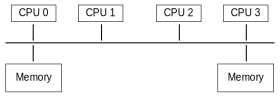
\includegraphics{memorder/SystemArchBus}}
\caption{Global System Bus And Multi-Copy Atomicity}
\label{fig:memorder:Global System Bus And Multi-Copy Atomicity}
\end{figure}

\emph{Multicopy atomic}~\cite{Stone:1995:SP:623262.623912} 플랫폼에서 돌아가는
쓰레드들은 스토어들의 순서에 대해서는 심지어 서로 다른 변수들에 대한 것조차도
동의를 할 것이 보장됩니다.
그런 시스템에 대한 유용한 상상의 모델은
Figure~\ref{fig:memorder:Global System Bus And Multi-Copy Atomicity}
에 보인 싱글 버스 아키텍쳐 같은 시스템입니다.
각각의 스토어가 버스로의 메세지를 낸다면, 그리고 이 버스가 한번에 하나의
스토어만 처리할 수 있다면, 모든 CPU 들은 모든 스토어에 대해 각각 관측한 순서가
동일할 겁니다.
불행히도, 그림에 보인 것처럼 스토어 버퍼나 캐시조차 없이 컴퓨터 시스템을
만드는건 빙하같은 계산속도가 나오게 할겁니다.
따라서 multicopy atomicity 를 제공하는데 흥미를 갖는 CPU 제조사들은 그대신 약간
더 완화된 \emph{other-multicopy atomicity}~\cite[Section B2.3]{ARMv8A:2017} 를
제공하고자 하게 되는데, 여기선 특정 스토어를 수행하는 CPU 는 모든 스토어들의
순서에 대한 CPU 들의 동의로부터 배제될 수 있게 해줍니다.
이는 CPU 들 중 일부만 스토어를 수행한다면, 다른 CPU 들은 스토어들의 순서에
동의함을 의미하는데, 따라서 ``other-multicopy atomicity'' 의 ``other'' 가
존재하는 겁니다.
Multicopy-atomic 플랫폼들과 달리, other-multicopy-atomic 플랫폼에서는, 스토어를
수행하는 CPU는 자신의 스토어를 더 빨리 관측할 수 있어서, 나중의 로드가 새로
스토어된 값을 스토어 버퍼로부터 곧바로 얻어올 수 있음을 의미합니다.
이는 끔찍한 플랫폼은 피할 수 있게 해줍니다.
\iffalse

Threads running on a \emph{multicopy atomic}~\cite{Stone:1995:SP:623262.623912}
platform are guaranteed
to agree on the order of stores, even to different variables.
A useful mental model of such a system is the single-bus architecture
shown in
Figure~\ref{fig:memorder:Global System Bus And Multi-Copy Atomicity}.
If each store resulted in a message on the bus, and if the bus could
accommodate only one store at a time, then any pair of CPUs would
agree on the order of all stores that they observed.
Unfortunately, building a computer system as shown in the figure,
without store buffers or even caches, would result in glacial computation.
CPU vendors interested in providing multicopy atomicity have therefore
instead provided the slightly weaker
\emph{other-multicopy atomicity}~\cite[Section B2.3]{ARMv8A:2017},
which excludes the CPU doing a given store from the requirement that all
CPUs agree on the order of all stores.
This means that if only a subset of CPUs are doing stores, the
other CPUs will agree on the order of stores, hence the ``other''
in ``other-multicopy atomicity''.
Unlike multicopy-atomic platforms, within other-multicopy-atomic platforms,
the CPU doing the store is permitted to observe its
store early, which allows its later loads to obtain the newly stored
value directly from the store buffer.
This in turn avoids abysmal performance.
\fi

\QuickQuiz{}
	Multicopy atomic 와 다른 multicopy atomic 사이의 다른 동작에 대한
	특정한 예를 들어볼 수 있겠습니까?
	\iffalse

	Can you give a specific example showing different behavior for
	multicopy atomic on the one hand and other-multicopy atomic
	on the other?
	\fi
\QuickQuizAnswer{
\begin{listing}[tbp]
{ \scriptsize
\begin{verbbox}[\LstLineNo]
C C-MP-OMCA+o-o-o+o-rmb-o

{
}

P0(int *x, int *y)
{
  int r0;

  WRITE_ONCE(*x, 1);
  r0 = READ_ONCE(*x);
  WRITE_ONCE(*y, r0);
}

P1(int *x, int *y)
{
  int r1;
  int r2;

  r1 = READ_ONCE(*y);
  smp_rmb();
  r2 = READ_ONCE(*x);
}

exists (1:r1=1 /\ 1:r2=0)
\end{verbbox}
}
\centering
\theverbbox
\caption{Litmus Test Distinguishing Multicopy Atomic From Other Multicopy Atomic}
\label{lst:memorder:Litmus Test Distinguishing Multicopy Atomic From Other Multicopy Atomic}
\end{listing}

	Listing~\ref{lst:memorder:Litmus Test Distinguishing Multicopy Atomic From Other Multicopy Atomic}
	(\path{C-MP-OMCA+o-o-o+o-rmb-o.litmus})
	이 그런 테스트를 보입니다.

	Multicopy-atomic 플랫폼에서, \co{P0()} 의 line~10 에서의 \co{x} 로의
	스토어는\co{P0()} 와 \co{P1()} 에게 동시에 보여야만 합니다.
	이 스토어는 \co{P0()} 에게 line~11 에서야 보이게 되고, line~12 에서의
	\co{P0()} 의 \co{y} 로의 스토어 전에, \co{P0()} 의 \co{x} 로의 스토어는
	\co{P1()} 을 포함해서 \co{y} 로의 스토어 전에 보여야만 합니다.
	따라서, line~20 에서 \co{P1()} 의 \co{y} 로부터의 로드가 값 1을
	리턴하면, line~21 에서의 \co{smp_rmb()} 가 이 두 로드의 수행 순서를
	강제하므로, line~22 에서의 \co{x} 역시 그래야만 합니다.
	따라서, line~25 의 \co{exists} 절은 multicopy-atomic 플랫폼에선느
	발동되지 않습니다.

	반면, other-multicopy-atomic 플랫폼에서는 \co{P0()} 가 자신의 스토어를
	일찍 볼 수 있으므로, \co{P1()} 이 이 두개의 스토어를 보는 순서에
	대해서는 제약이 없어서 \co{exists} 절이 발동될 수 있을 겁니다.
	\iffalse

	Listing~\ref{lst:memorder:Litmus Test Distinguishing Multicopy Atomic From Other Multicopy Atomic}
	(\path{C-MP-OMCA+o-o-o+o-rmb-o.litmus})
	shows such a test.

	On a multicopy-atomic platform, \co{P0()}'s store to \co{x} on
	line~10 must become visible to both \co{P0()} and \co{P1()}
	simultaneously.
	Because this store becomes visible to \co{P0()} on line~11, before
	\co{P0()}'s store to \co{y} on line~12, \co{P0()}'s store to
	\co{x} must become visible before its store to \co{y} everywhere,
	including \co{P1()}.
	Therefore, if \co{P1()}'s load from \co{y} on line~20 returns the
	value 1, so must its load from \co{x} on line~22, given that
	the \co{smp_rmb()} on line~21 forces these two loads to execute
	in order.
	Therefore, the \co{exists} clause on line~25 cannot trigger on a
	multicopy-atomic platform.

	In contrast, on an other-multicopy-atomic platform, \co{P0()}
	could see its own store early, so that there would be no constraint
	on the order of visibility of the two stores from to \co{P1()},
	which in turn allows the \co{exists} clause to trigger.
	\fi
} \QuickQuizEnd

모든 플랫폼이 어떤 형태의 multi-copy atomicity 를 제공하는 시대가 올수도
있겠습니다만, 그 사이에는 multicopy-atomic 이 아닌 플랫폼이 존재할 것이고,
따라서 소프트웨어는 그걸 잘 다뤄야 합니다.
\iffalse

Perhaps there will come a day when all platforms provide some flavor
of multi-copy atomicity, but
in the meantime, non-multicopy-atomic platforms do exist, and so software
does need to deal with them.
\fi

\begin{listing}[tbp]
{ \scriptsize
\begin{verbbox}[\LstLineNo]
C C-WWC+o+o-data-o+o-addr-o

{
int a = 0;
int b = 0;
int *c = &b;
int *x = &a;
int *y = &b;
}

P0(int **x)
{
  WRITE_ONCE(*x, x);
}

P1(int **x, int **y)
{
  int *r1;

  r1 = READ_ONCE(*x);
  WRITE_ONCE(*y, r1);
}

P2(int **y, int **c)
{
  int *r2;

  r2 = READ_ONCE(*y);
  WRITE_ONCE(*r2, c);
}

exists(1:r1=x /\ 2:r2=x /\ x=x)
\end{verbbox}
}
\centering
\theverbbox
\caption{WWC Litmus Test With Dependencies (No Ordering)}
\label{lst:memorder:WWC Litmus Test With Dependencies (No Ordering)}
\end{listing}

Listing~\ref{lst:memorder:WWC Litmus Test With Dependencies (No Ordering)}
(\path{C-WWC+o+o-data-o+o-addr-o.litmus})
은 multicopy atomicity 를 보이고 있는데, multicopy-atomic 플랫폼 위에서라면
line~32 의 \co{exists} 절은 발동될 수 없습니다.
반면에, multicopy-atomic 이 아닌 플랫폼에서 이 \co{exists} 절은 \co{P1()} 의
액세스들은 data dependency 로 순서잡혀지고 \co{P2()} 의 액세스들은 address
dependency 로 순서잡혀짐에도 발동될 수 있습니다.
Multicopy atomicity 의 정의는 모든 쓰레드가 스토어의 순서에 동의할 것을, 즉
모든 스토어가 모든 쓰레드에 같은 시간에 도착하는 것으로 생각될 수도 있을 것을
요구함을 다시 이야기 드립니다.
따라서, multicopy-atomic 이 아닌 플랫폼은 다른 쓰레드에 다른 시간에 도착하는
스토어가 있을 수 있습니다.
특히, \co{P0()} 의 스토어는 \co{P2()} 에 도착하기 훨씬 전에 \co{P1()} 에 도착할
수도 있는데, 이는 \co{P1()} 의 스토어가 \co{P0()} 의 스토어보다 먼저 \co{P2()}
에 도착할 확률을 높입니다.
\iffalse

Listing~\ref{lst:memorder:WWC Litmus Test With Dependencies (No Ordering)}
(\path{C-WWC+o+o-data-o+o-addr-o.litmus})
demonstrates multicopy atomicity, that is, on a multicopy-atomic platform,
the \co{exists} clause on line~32 cannot trigger.
In contrast, on a non-multicopy-atomic
platform this \co{exists} clause can trigger, despite
\co{P1()}'s accesses being ordered by a data dependency and \co{P2()}'s
accesses being ordered by an address dependency.
Recall that the definition of multicopy atomicity requires that all
threads agree on the order of stores, which can be thought of as
all stores reaching all threads at the same time.
Therefore, a non-multicopy-atomic platform can have a store reach
different threads at different times.
In particular, \co{P0()}'s store might reach \co{P1()} long before it
reaches \co{P2()}, which raises the possibility that \co{P1()}'s store
might reach \co{P2()} before \co{P0()}'s store does.
\fi

\begin{figure}[tb]
\centering
\resizebox{3.0in}{!}{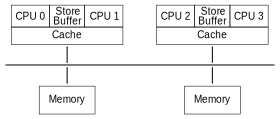
\includegraphics{memorder/NonMCAplatform}}
\caption{Shared Store Buffers And Multi-Copy Atomicity}
\label{fig:memorder:Shared Store Buffers And Multi-Copy Atomicity}
\end{figure}

이는 왜 일반적인 물리 법칙의 제한을 받는 실제 시스템이
Listing~\ref{lst:memorder:WWC Litmus Test With Dependencies (No Ordering)}
의 \co{exists} 절을 발동시키는지에 대한 의문을 낳습니다.
그런 실제 시스템에 대한 그림이
Figure~\ref{fig:memorder:Shared Store Buffers And Multi-Copy Atomicity} 에
그려져 있습니다.
CPU~0 와 CPU~1 은 스토어 버퍼를 공유하며, CPU~2 와~3 도 그렇습니다.
이는 CPU~1 은 이 스토어 버퍼로부터 값을 로드할 수 있으며, 따라서 CPU~0 가
스토어한 값을 곧바로 볼 가능성이 있습니다.
반면에, CPU~2 와~3 은 연관된 캐시 라인이 새로운 값을 자신에게 가져올 때까지
기다려야 합니다.
\iffalse

This leads to the question of why a real system constrained by the
usual laws of physics would ever trigger the \co{exists} clause of
Listing~\ref{lst:memorder:WWC Litmus Test With Dependencies (No Ordering)}.
The cartoonish diagram of a such a real system is shown in
Figure~\ref{fig:memorder:Shared Store Buffers And Multi-Copy Atomicity}.
CPU~0 and CPU~1 share a store buffer, as do CPUs~2 and~3.
This means that CPU~1 can load a value out of the store buffer, thus
potentially immediately seeing a value stored by CPU~0.
In contrast, CPUs~2 and~3 will have to wait for the corresponding cache
line to carry this new value to them.
\fi

\QuickQuiz{}
	대체 누가 공유된 스토어 버퍼를 갖는 시스템을 설계할 \emph{생각} 따위를
	하겠어요???
	\iffalse

	Then who would even \emph{think} of designing a system with shared
	store buffers???
	\fi
\QuickQuizAnswer{
	이는 코어당 여러 하드웨어 쓰레드를 갖는 시스템에서는 매우 자연스러운
	설계입니다.
	하드웨어의 관점에서는 자연스럽습니다, 이게요!
	\iffalse

	This is in fact a very natural design for any system having
	multiple hardware threads per core.
	Natural from a hardware point of view, that is!
	\fi
} \QuickQuizEnd

\begin{table*}
\small
\centering\OneColumnHSpace{-0.8in}
\begin{tabular}{r||l|l|l|l||l|l|l}
	& \tco{P0()} & \multicolumn{2}{c|}{\tco{P0()} \& \tco{P1()}} & \tco{P1()} & \multicolumn{3}{c}{\tco{P2()}} \\
	\cline{2-8}
	& Instruction & Store Buffer & Cache & Instruction &
			Instruction & Store Buffer & Cache \\
	\hline
	\hline
	1 & (Initial state) & & \tco{y==&b} &
		(Initial state) &
			(Initial state) & & \tco{x==&a} \\
	\hline
	2 & \tco{x = &x;} & \tco{x==&x} & \tco{y==&b} &
		 & & & \tco{x==&a} \\
	\hline
	3 & (Read-Invalidate \tco{x}) & \tco{x==&x} & \tco{y==&b} & \tco{r1 = x} (\tco{&x})
		 & & & \tco{x==&a} \\
	\hline
	4 &  & \tco{x==&x} \tco{y==&x} & \tco{y==&b} & \tco{y = r1}
		 & \tco{r2 = y} & & \tco{x==&a} \\
	\hline
	5 &  & \tco{x==&x} & \tco{y==&x} & (Finish store)
		 & (Read \tco{y}) & & \tco{x==&a} \\
	\hline
	6 & & \tco{x==&x} & \tco{y==&x} &
		 & (\tco{r2==&x}) & & \tco{x==&a} \tco{y==&x} \\
	\hline
	7 & & \tco{x==&x} & \tco{y==&x} &
		 & \tco{*r2 = &c} & \tco{y==&c} & \tco{x==&a} \tco{y==&x} \\
	\hline
	8 & & \tco{x==&x} & \tco{y==&x} &
		 & (Read Invalidate \tco{y}) & \tco{y==&c} & \tco{x==&a} \tco{y==&x} \\
	\hline
	9 & & \tco{x==&x} &  &
		 &  & \tco{y==&c} & \tco{x==&a} \tco{y==&x} \\
	\hline
	10 & & \tco{x==&x} &  &
		 & (Finish store) & & \tco{x==&a} \tco{y==&c} \\
	\hline
	11 & & \tco{x==&x} & \tco{x==&a} &
		 & (Respond \co{x}) & & \tco{y==&c} \\
	\hline
	12 & (Finish store) & & \tco{x==&x} &
		 &  & & \tco{y==&c} \\
\end{tabular}
\caption{Memory Ordering: WWC Sequence of Events}
\label{tab:memorder:Memory Ordering: WWC Sequence of Events}
\end{table*}

Table~\ref{tab:memorder:Memory Ordering: WWC Sequence of Events}
은
Listing~\ref{lst:memorder:WWC Litmus Test With Dependencies (No Ordering)}
의 \co{exists} 절이 발동될 수 있는 일련의 이벤트를 보입니다.
이 일련의 이벤트는 \co{P0()} 와 \co{P1()} 이
Figure~\ref{fig:memorder:Shared Store Buffers And Multi-Copy Atomicity} 에 보인
방식으로 캐시와 스토어 버퍼를 공유한다는 점에 상당히 의존적입니다.
\iffalse

Table~\ref{tab:memorder:Memory Ordering: WWC Sequence of Events}
shows one sequence of events that can result in the \co{exists} clause in
Listing~\ref{lst:memorder:WWC Litmus Test With Dependencies (No Ordering)}
triggering.
This sequence of events will depend critically on \co{P0()} and
\co{P1()} sharing both cache and a store buffer in the manner shown in
Figure~\ref{fig:memorder:Shared Store Buffers And Multi-Copy Atomicity}.
\fi

\QuickQuiz{}
	하지만 \co{P0()} 와 \co{P1()} 은 스토어 버퍼와 캐시를 공유해야 하는데
	\co{P2()} 는 자기만의 캐시와 스토어 버퍼를 갖는다는게 공평한가요???
	\iffalse

	But just how is it fair that \co{P0()} and \co{P1()} must share a store
	buffer and a cache, but \co{P2()} gets one each of its very own???
	\fi
\QuickQuizAnswer{
	어쩌면
	Figure~\ref{fig:memorder:Shared Store Buffers And Multi-Copy Atomicity}
	에 보인 것처럼 \co{P3()} 가 존재해서 \co{P2()} 의 스토어 버퍼와 캐시를
	공유할 수도 있을 겁니다.  하지만 꼭 그래야 하는 건 아니죠.
	일부 플랫폼은 서로 다른 코어들이 서로 다른 수의 쓰레드들을 불능화
	시키는걸 가능하게 해서, 하드웨어가 당장 처리해야할 워크로드의 필요에
	맞게 조정될 수 있게 합니다.
	예를 들어, 워크로드의 싱글 쓰레드로 돌아가는 중요한 지점은 하나의
	쓰레드만 돌아갈 수 있는 코어에 할당되어서 이 워크로드의 해당 부분을 이
	하나의 쓰레드가 해당 코어의 모든 가능한 자원을 사용할 수 있게 할 수
	있을 겁니다.
	워크로드의 더 높은 병렬성을 갖지만 캐시미스에 취약한 부분은 더 나은
	처리량을 제공하기 위해 모든 하드웨어 쓰레드를 사용할 수 있는 코어들에
	할당될 수 있을 겁니다.
	이렇게 향상된 처리량은 하나의 하드웨어 쓰레드가 캐시 미스에 의해 멈춰
	있는 동안, 다른 하드웨어 쓰레드는 진행을 이룰 수 있기 때문이기도
	할겁니다.

	이런 경우, 성능 요구사항은 독특한 사람의 관점에서의 공평성보다
	우선합니다.
	\iffalse

	Presumably there is a \co{P3()}, as is in fact shown in
	Figure~\ref{fig:memorder:Shared Store Buffers And Multi-Copy Atomicity},
	that shares \co{P2()}'s store buffer and cache.
	But not necessarily.
	Some platforms allow different cores to disable different numbers
	of threads, allowing the hardware to adjust to the needs of the
	workload at hand.
	For example, a single-threaded critical-path portion of the workload
	might be assigned to a core with only one thread enabled, thus
	allowing the single thread running that portion of the workload
	to use the entire capabilities of that core.
	Other more highly parallel but cache-miss-prone portions of the
	workload might be assigned to cores with all hardware threads
	enabled to provide improved throughput.
	This improved throughput could be due to the fact that while one
	hardware thread is stalled on a cache miss, the other hardware
	threads can make forward progress.

	In such cases, performance requirements override quaint human
	notions of fairness.
	\fi
} \QuickQuizEnd

Row~1 은 최초의 상태를 보이는데, \co{y} 는 \co{P0()} 와 \co{P1()} 의 공유된
캐시에, \co{x} 의 최초 값은 \co{P2()} 의 캐시에 있습니다.

Row~2 는 \co{P0()} 의 line~13 에서의 스토어가 수행된 직후의 효과를 보입니다.
\co{x} 를 담고 있는 캐시라인은 \co{P0()} 와 \co{P1()} 의 공유 캐시에 있지
않으므로, 새로운 값 (\co{&x}) 은 해당 CPU 들의 공유 스토어 버퍼에 저장됩니다.

Row~3 는 두개의 사건을 보입니다.
먼저, \co{P0()} 는 \co{x} 의 새로운 값을 공유 스토어 버퍼에서 내려보낼 수
있게끔 \co{x} 를 담고 있는 캐시라인을 얻어오기 위해 read-invalidate
오퍼레이션을 날립니다.
이어서, \co{P1()} 은 \co{x} 를 읽어오는데 (line~20), 이 오퍼레이션은 \co{x} 의
새로운 값을 공유 스토어 버퍼에서 곧바로 얻어올 수 있기 때문에 즉각적으로
완료됩니다.
\iffalse

Row~1 shows the initial state, with the initial value of \co{y} in
\co{P0()}'s and \co{P1()}'s shared cache, and the initial value of \co{x} in
\co{P2()}'s cache.

Row~2 shows the immediate effect of \co{P0()} executing its store on line~13.
Because the cacheline containing \co{x} is not in \co{P0()}'s and \co{P1()}'s
shared cache, the new value (\co{&x})is stored in the shared store buffer.

Row~3 shows two transitions.
First, \co{P0()} issues a read-invalidate operation to fetch the cacheline
containing \co{x} so that it can flush the new value for \co{x} out of
the shared store buffer.
Second, \co{P1()} loads from \co{x} (line~20), an operation that completes
immediately because the new value of \co{x} is immediately available
from the shared store buffer.
\fi

Row~4 또한 두개의 사건을 보입니다.
먼저, \co{P1()} 이 \co{y} 로의 스토어 (line~21) 을 수행한 직후의 효과로, 이
새로운 값은 공유 스토어 버퍼에 저장됨을 보입니다.
이어서, \co{P2()} 의 \co{y} 로부터의 로드 (line~28) 를 보입니다.

Row~5 는 두개의 사건의 이후 흐름을 보입니다.
먼저, \co{P1()} 은 \co{y} 로의 스토어를 완료하고, 공유 스토어 버퍼에서 캐시로
값을 내림을 보입니다.
또한, \co{P2()} 의 \co{x} 를 담고 있는 캐시라인으로의 요청을 보입니다.

Row~6 는 \co{P2()} 가 \co{y} 를 담고 있는 캐시라인을 받아서 \co{r2} 로의 로드를
마칠 수 있게 해주는데, 이 로드는 \co{&x} 의 값을 가져오게 됩니다.

Row~7 은 \co{P2()} 가 \co{y} 로의 스토어 (line~29) 를 시작하는 것을 보이는데,
이 새로운 값은 스토어 버퍼에 저장됩니다.
\iffalse

Row~4 also shows two transitions.
First, it shows the immediate effect of \co{P1()} executing its store to
\co{y} (line~21), placing the new value into the shared store buffer.
Second, it shows the start of \co{P2()}'s load from \co{y} (line~28).

Row~5 continues the tradition of showing two transitions.
First, it shows \co{P1()} complete its store to \co{y}, flushing
from the shared store buffer to the cache.
Second, it shows \co{P2()} request the cacheline containing \co{x}.

Row~6 shows \co{P2()} receive the cacheline containing \co{y}, allowing
it to finish its load into \co{r2}, which takes on the value \co{&x}.

Row~7 shows \co{P2()} start executing its store to \co{y} (line~29), placing the
new value in is store buffer.
\fi

Row~8 은 \co{P2()} 가 스토어를 끝내기 위해 \co{y} 를 담고 있는 캐시라인에 대해
배타적 소유권을 요청하는 모습 (``Read Invalidate'') 을 보입니다.

Row~9 은 \co{y} 를 담고 있는 캐시라인이 공유 캐시에서 사라지는 모습을 보이는데,
이로써 \co{P2()} 는 이제 배타적 소유권을 갖습니다.

Row~10 은 \co{P2()} 가 \co{y} 로의 스토어를 그 값을 자신의 스토어 버퍼에서
캐시로 내려보냄으로써 완료하는 것을 보입니다.

Row~11 은 \co{P2()} 가 \emph{마침내} row~3 에서 만들어진, \co{P0()} 의 \co{x}
를 담고 있는 캐시라인에 대한 요청에 응답을 하는 걸 보입니다.

마지막으로, row~12 는 \co{P0()} 가 자신의 스토어를 마무리 지어서, \co{x} 에
대한 자신의 값을 공유 스토어 버퍼에서 공유 캐시로 내려보내는 것을 보입니다.

Line~32 의 \co{exists} 절이 발동됨 역시 알아두시기 바랍니다.
\co{r1} 과 \co{r2} 의 값들은 모두 \co{x} 의 주소이고, \co{x} 의 마지막 값은
또한 \co{x} 의 주소입니다.
이 이상한 결과는 \co{P0()} 의 \co{x} 에 대한 새로운 값이 \co{P2()} 와 이야기
하기 전에 \co{P1()} 에게 전달되었기 때문에 발생했습니다.
\iffalse

Row~8 shows \co{P2()} requesting exclusive ownership (``Read Invalidate'')
for the cacheline containing \co{y} in order to finish its store.

Row~9 shows the cacheline containing \co{y} removed from the shared cache,
so that \co{P2()} now has exclusive ownership.

Row~10 shows \co{P2()} completing its store to \co{y}, flushing the value
from its store buffer to its cache.

Row~11 shows \co{P2()} \emph{finally} responding to \co{P0()}'s request for
the cacheline containing \co{x}, which was made way back up on row~3.

Finally, row~12 shows \co{P0()} finish its store, flushing its value of
\co{x} from the shared store buffer to the shared cache.

Note well that the \co{exists} clause on line~32 has triggered.
The values of \co{r1} and \co{r2} are both the address of \co{x}, and
the final value of \co{x} is also the address of \co{x}.
This strange result occurred because \co{P0()}'s new value of \co{x} was
communicated to \co{P1()} long before it was communicated to \co{P2()}.
\fi

\QuickQuiz{}
	Table~\ref{tab:memorder:Memory Ordering: WWC Sequence of Events}
	대로라면, \co{P1()} 과 \co{P2()} 의 스토어는 그렇게 빨리 끝나는데
	\co{P0()} 의 스토어는 왜 그렇게 오래 걸리나요?
	달리 말하자면,
	Listing~\ref{lst:memorder:WWC Litmus Test With Dependencies (No Ordering)}
	의 line~32 에 있는 \co{exists} 절은 정말로 실제 시스템에서도
	발동되는건가요?
	\iffalse

	Referring to
	Table~\ref{tab:memorder:Memory Ordering: WWC Sequence of Events},
	why on earth would \co{P0()}'s store take so long to complete when
	\co{P1()}'s and \co{P2()}'s stores complete so quickly?
	In other words, does the \co{exists} clause on line~32 of
	Listing~\ref{lst:memorder:WWC Litmus Test With Dependencies (No Ordering)}
	really trigger on real systems?
	\fi
\QuickQuizAnswer{
	정말로 발동될 수 있다는 사실을 받아들여야 합니다.
	Akira Yokosawa 는 \co{litmus7} 이라는 도구를 사용해 Power8 시스템에서
	이 리트머스 테스트를 돌려봤습니다.
	100,000,000,000 번의 시도 중에, 1,119 번 \co{exists} 절이
	발동되었습니다.
	따라서, \co{exists} 절의 발동 확률은 백만번에 한번도 아니고, 일억번 중
	한번입니다.
	하지만 실제 시스템에서도 발동된다는 것은 사실입니다.
	\iffalse

	You need to face the fact that it really can trigger.
	Akira Yokosawa used the \co{litmus7} tool to run this litmus test
	on a Power8 system.
	Out of 100,000,000,000 runs, 1,119 triggered the \co{exists}
	clause.
	Thus, triggering the \co{exists} clause is not merely a one-in-a-million
	occurrence, but rather a one-in-a-hundred-million occurrence.
	But it nevertheless really does trigger on real systems.
	\fi
} \QuickQuizEnd

의존성이 순서를 제공하긴 하지만, 각자의 쓰레드 스스로에 대해서만 제공하기
때문에 이 반직관적인 결과가 일어납니다.
이 세개 쓰레드 예제는 더 강한 순서 규칙을 필요로 하는데,
Section~\ref{sec:memorder:Cumulativity}
부터~\ref{sec:memorder:Release-Acquire Chains} 까지의 주제가 이를 다룹니다.
\iffalse

This counter-intuitive result happens because although dependencies
do provide ordering, they provide it only within the confines of their
own thread.
This three-thread example requires stronger ordering, which
is the subject of
Sections~\ref{sec:memorder:Cumulativity}
through~\ref{sec:memorder:Release-Acquire Chains}.
\fi

\subsubsection{Cumulativity}
\label{sec:memorder:Cumulativity}

The three-thread example shown in
Listing~\ref{lst:memorder:WWC Litmus Test With Dependencies (No Ordering)}
requires \emph{cumulative} ordering, or \emph{cumulativity}.
A cumulative barrier orders not just any given access preceding it, but
also earlier accesses by any thread to that same variable.

\begin{listing}[tbp]
{ \scriptsize
\begin{verbbox}[\LstLineNo]
C C-WWC+o+o-r+o-addr-o

{
int a = 0;
int b = 0;
int *c = &b;
int *x = &a;
int *y = &b;
}

P0(int **x)
{
  WRITE_ONCE(*x, x);
}

P1(int **x, int **y)
{
  int *r1;

  r1 = READ_ONCE(*x);
  smp_store_release(y, r1);
}

P2(int **y, int **c)
{
  int *r2;

  r2 = READ_ONCE(*y);
  WRITE_ONCE(*r2, c);
}

exists(1:r1=x /\ 2:r2=x /\ x=x)
\end{verbbox}
}
\centering
\theverbbox
\caption{WWC Litmus Test With Release}
\label{lst:memorder:WWC Litmus Test With Release}
\end{listing}

Dependencies do not provide cumulativity,
which is why the ``C'' column is blank for
both the \co{READ_ONCE()} and the \co{smp_read_barrier_depends()} rows
of Table~\ref{tab:memorder:Linux-Kernel Memory-Ordering Cheat Sheet}.
However, as indicated by the ``C'' in their ``C'' column,
release operations do provide cumulativity.
Therefore,
Listing~\ref{lst:memorder:WWC Litmus Test With Release}
(\path{C-WWC+o+o-r+o-addr-o.litmus})
substitutes a release operation for
Listing~\ref{lst:memorder:WWC Litmus Test With Dependencies (No Ordering)}'s
data dependency.
Because the release operation is cumulative, its ordering applies not only to
Listing~\ref{lst:memorder:WWC Litmus Test With Release}'s
load from \co{x} by \co{P1()} on line~20, but also to its store to \co{x}
by \co{P0()} on line~13---but only if that load returns the value stored,
which in this case is the address of \co{x}, which matches the \co{1:r1=x}
in the \co{exists} clause on line~32.
This means that \co{P2()}'s address dependency suffices to force the
store to \co{x} on line~29 to happen after the store on line~13, so
that the final value of \co{x} is the address of \co{c}, which
in turn prevents the \co{exists} clause from triggering.

\begin{figure*}[htbp]
\centering
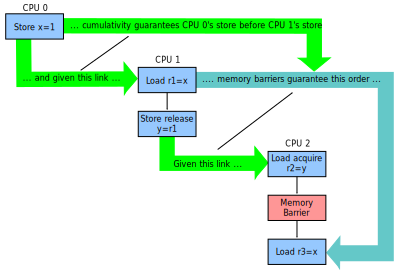
\includegraphics{memorder/memorybarriercum}
\caption{Cumulativity}
\label{fig:memorder:Cumulativity}
\end{figure*}

These ordering constraints are depicted graphically in
Figure~\ref{fig:memorder:Cumulativity}.
Note also that cumulativity is not limited to a single step back in time.
If there was another load from \co{x} or store to \co{x} from any thread
that came before the store on line~13, that prior load or store would also
be ordered before the store on line~32, though only if both \co{r1} and
\co{r2} both end up containing the address of \co{x}.

In short, use of cumulative ordering operations can suppress
non-multicopy-atomic behaviors in some situations.
Cumulativity nevertheless has limits, which are examined in the next section.

\subsubsection{Propagation}
\label{sec:memorder:Propagation}

\begin{listing}[tbp]
{ \scriptsize
\begin{verbbox}[\LstLineNo]
C C-W+RWC+o-r+a-o+o-mb-o

{
int x = 0;
int y = 0;
int z = 0;
}

P0(int *x, int *y)
{
  WRITE_ONCE(*x, 1);
  smp_store_release(y, 1);
}

P1(int *y, int *z)
{
  int r1;
  int r2;

  r1 = smp_load_acquire(y);
  r2 = READ_ONCE(*z);
}

P2(int *z, int *x)
{
  int r3;

  WRITE_ONCE(*z, 1);
  smp_mb();
  r3 = READ_ONCE(*x);
}

exists(1:r1=1 /\ 1:r2=0 /\ 2:r3=0)
\end{verbbox}
}
\centering
\theverbbox
\caption{W+RWC Litmus Test With Release (No Ordering)}
\label{lst:memorder:W+RWC Litmus Test With Release (No Ordering)}
\end{listing}

Listing~\ref{lst:memorder:W+RWC Litmus Test With Release (No Ordering)}
(\path{C-W+RWC+o-r+a-o+o-mb-o.litmus})
shows the limitations of cumulativity and of store-release,
even with a full memory barrier helping out.
The problem is that although the \co{smp_store_release()} on
line~12 has cumulativity, and although that cumulativity does
order \co{P2()}'s load on line~30, the \co{smp_store_release()}'s
ordering cannot propagate through the combination of \co{P1()}'s
load (line~21) and \co{P2()}'s store (line~28).
This means that the \co{exists} clause on line~33 really can trigger.

\QuickQuiz{}
	But it is not necessary to worry about propagation unless
	there are at least three threads in the litmus test, right?
\QuickQuizAnswer{
\begin{listing}[tbp]
{ \scriptsize
\begin{verbbox}[\LstLineNo]
C C-R+o-wmb-o+o-mb-o
{
}

P0(int *x0, int *x1)
{
  WRITE_ONCE(*x0, 1);
  smp_wmb();
  WRITE_ONCE(*x1, 1);
}


P1(int *x0, int *x1)
{
  int r2;

  WRITE_ONCE(*x1, 2);
  smp_mb();
  r2 = READ_ONCE(*x0);
}

exists (1:r2=0 /\ x1=2)
\end{verbbox}
}
\centering
\theverbbox
\caption{R Litmus Test With Write Memory Barrier (No Ordering)}
\label{lst:memorder:R Litmus Test With Write Memory Barrier (No Ordering)}
\end{listing}
	Wrong.

	Listing~\ref{lst:memorder:R Litmus Test With Write Memory Barrier (No Ordering)}
	(\path{C-R+o-wmb-o+o-mb-o.litmus})
	shows a two-thread litmus test that requires propagation due to
	the fact that it only has store-to-store and load-to-store
	relationships between its pair of threads.
	Even though \co{P0()} is fully ordered by the \co{smp_wmb()} and
	\co{P1()} is fully ordered by the \co{smp_mb()}, the
	counter-temporal nature of the relationships means that
	the \co{exists} clause on line~22 really can trigger.
	To prevent this triggering, the \co{smp_wmb()} on line~8
	must become an \co{smp_mb()}, bringing propagation into play
	twice, once for each non-temporal relationship.
} \QuickQuizEnd

\begin{figure}[htbp]
\centering
\resizebox{\columnwidth}{!}{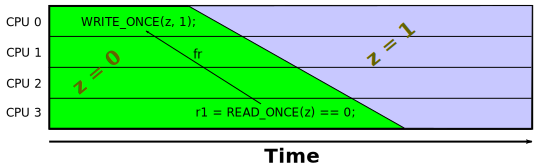
\includegraphics{memorder/fr}}
\caption{Load-to-Store is Counter-Temporal}
\label{fig:memorder:Load-to-Store is Counter-Temporal}
\end{figure}

This situation might seem completely counter-intuitive, but keep
in mind that the speed of light is finite and computers are of
non-zero size.
It therefore takes time for the effect of the \co{P2()}'s store to
\co{z} to propagate to \co{P1()}, which in turn means that it is possible
that \co{P1()}'s read from \co{z} happens much later in time, but
nevertheless still sees the old value of zero.
This situation is depicted in
Figure~\ref{fig:memorder:Load-to-Store is Counter-Temporal}:
Just because a load sees the old value does \emph{not} mean that
this load executed at an earlier time than did the store of the
new value.

Note that
Listing~\ref{lst:memorder:W+RWC Litmus Test With Release (No Ordering)}
also shows the limitations of memory-barrier pairing, given that
there are not two but three processes.
These more complex litmus tests can instead be said to have \emph{cycles},
where memory-barrier pairing is the special case of a two-thread cycle.
The cycle in
Listing~\ref{lst:memorder:W+RWC Litmus Test With Release (No Ordering)}
goes through \co{P0()} (lines~11 and~12), \co{P1()} (lines~20 and~21),
\co{P2()} (lines~28, 29, and~30), and back to \co{P0()} (line~11).
The \co{exists} clause delineates this cycle:
the \co{1:r1=1} indicates that the \co{smp_load_acquire()} on line~20
returned the value stored by the \co{smp_store_release()} on line~12,
the \co{1:r2=0} indicates that the \co{WRITE_ONCE()} on line~28 came
too late to affect the value returned by the \co{READ_ONCE()} on line~21,
and finally the \co{2:r3=0} indicates that the
\co{WRITE_ONCE()} on line~11 came to late to affect the value returned
by the \co{READ_ONCE()} on line~30.
In this case, the fact that the \co{exists} clause can trigger means that
the cycle is said to be \emph{allowed}.
In contrast, in cases where the \co{exists} clause cannot trigger,
the cycle is said to be \emph{prohibited}.

\begin{listing}[tbp]
{ \scriptsize
\begin{verbbox}[\LstLineNo]
C C-W+RWC+o-mb-o+a-o+o-mb-o

{
int x = 0;
int y = 0;
int z = 0;
}

P0(int *x, int *y)
{
  WRITE_ONCE(*x, 1);
  smp_mb();
  WRITE_ONCE(*y, 1);
}

P1(int *y, int *z)
{
  int r1;
  int r2;

  r1 = smp_load_acquire(y);
  r2 = READ_ONCE(*z);
}

P2(int *z, int *x)
{
  int r3;

  WRITE_ONCE(*z, 1);
  smp_mb();
  r3 = READ_ONCE(*x);
}

exists(1:r1=1 /\ 1:r2=0 /\ 2:r3=0)
\end{verbbox}
}
\centering
\theverbbox
\caption{W+WRC Litmus Test With More Barriers}
\label{lst:memorder:W+WRC Litmus Test With More Barriers}
\end{listing}

But what if we need to keep the \co{exists} clause on line~33 of
Listing~\ref{lst:memorder:W+RWC Litmus Test With Release (No Ordering)}?
One solution is to replace \co{P0()}'s \co{smp_store_release()}
with an \co{smp_mb()}, which
Table~\ref{tab:memorder:Linux-Kernel Memory-Ordering Cheat Sheet}
shows to have not only cumulativity, but also propagation.
The result is shown in
Listing~\ref{lst:memorder:W+WRC Litmus Test With More Barriers}
(\path{C-W+RWC+o-mb-o+a-o+o-mb-o.litmus}).

\QuickQuiz{}
	But given that \co{smp_mb()} has the propagation property,
	why doesn't the \co{smp_mb()} on line~29 of
	Listing~\ref{lst:memorder:W+RWC Litmus Test With Release (No Ordering)}
	prevent the \co{exists} clause from triggering?
\QuickQuizAnswer{
	As a rough rule of thumb, the \co{smp_mb()} barrier's
	propagation property is sufficient to maintain ordering
	through only one store-to-load relationship between
	processes.
	Unfortunately,
	Listing~\ref{lst:memorder:W+RWC Litmus Test With Release (No Ordering)}
	has not one but two store-to-load relationships, with the
	first being from the \co{READ_ONCE()} on line~21 to the
	\co{WRITE_ONCE()} on line~28 and the second being from
	the \co{READ_ONCE()} on line~30 to the \co{WRITE_ONCE()}
	on line~11.
	Therefore, preventing the \co{exists} clause from triggering
	should be expected to require not one but two
	instances of \co{smp_mb()}.

	As a special exception to this rule of thumb, a release-acquire
	chain can have one load-to-store relationship between processes
	and still prohibit the cycle.
} \QuickQuizEnd

\begin{figure}[tbp]
\centering
\resizebox{\columnwidth}{!}{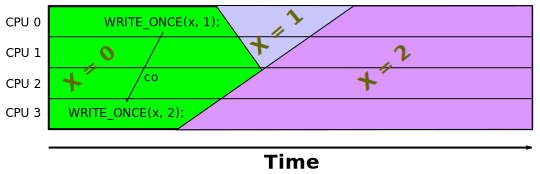
\includegraphics{memorder/co}}
\caption{Store-to-Store is Counter-Temporal}
\label{fig:memorder:Store-to-Store is Counter-Temporal}
\end{figure}

For completeness,
Figure~\ref{fig:memorder:Store-to-Store is Counter-Temporal}
shows that the ``winning'' store among a group of stores to the
same variable is not necessarily the store that started last.
This should not come as a surprise to anyone who carefully examined
Figure~\ref{fig:memorder:A Variable With More Simultaneous Values}.

But sometimes time is on our side, as shown in the next section.

\subsubsection{Happens-Before}
\label{sec:memorder:Happens-Before}

\begin{figure}[tbp]
\centering
\resizebox{\columnwidth}{!}{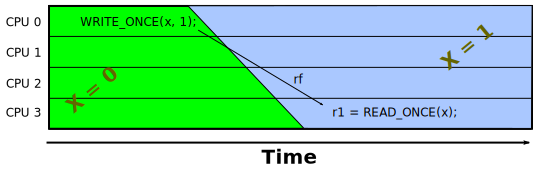
\includegraphics{memorder/rf}}
\caption{Store-to-Load is Temporal}
\label{fig:memorder:Store-to-Load is Temporal}
\end{figure}

As shown in
Figure~\ref{fig:memorder:Store-to-Load is Temporal},
on non-speculative platforms, if a load returns the value from a
particular store, then, courtesy of the finite speed of light and
the non-zero size of modern computing systems, the store absolutely
has to have executed at an earlier time than did the load.
This means that carefully constructed programs can rely on the
passage of time itself as an memory-ordering operation.

\begin{listing}[tbp]
{ \scriptsize
\begin{verbbox}[\LstLineNo]
C C-LB+a-o+o-data-o+o-data-o
{
}

P0(int *x0, int *x1)
{
  int r2;

  r2 = smp_load_acquire(x0);
  WRITE_ONCE(*x1, 2);
}


P1(int *x1, int *x2)
{
  int r2;

  r2 = READ_ONCE(*x1);
  WRITE_ONCE(*x2, r2);
}

P2(int *x2, int *x0)
{
  int r2;

  r2 = READ_ONCE(*x2);
  WRITE_ONCE(*x0, r2);
}

exists (0:r2=2 /\ 1:r2=2 /\ 2:r2=2)
\end{verbbox}
}
\centering
\theverbbox
\caption{LB Litmus Test With One Acquire}
\label{lst:memorder:LB Litmus Test With One Acquire}
\end{listing}

Of course, just the passage of time by itself is not enough, as
was seen in
Listing~\ref{lst:memorder:Load-Buffering Litmus Test (No Ordering)},
which has nothing but store-to-load relationships and still can
trigger its \co{exists} clause.
However, as long as each thread provides even the weakest possible
ordering, \co{exists} clause would not be able to trigger.
For example,
Listing~\ref{lst:memorder:LB Litmus Test With One Acquire}
(\path{C-LB+a-o+o-data-o+o-data-o.litmus})
shows \co{P0()} ordered with an \co{smp_load_acquire()} and
both \co{P1()} and \co{P2()} ordered with data dependencies.
These orderings, which are close to the top of
Table~\ref{tab:memorder:Linux-Kernel Memory-Ordering Cheat Sheet},
suffice to prevent the \co{exists} clause from triggering.

\QuickQuiz{}
	Can you construct a litmus test similar to that in
	Listing~\ref{lst:memorder:LB Litmus Test With One Acquire}
	that uses \emph{only} dependencies?
\QuickQuizAnswer{
	Listing~\ref{lst:memorder:LB Litmus Test With No Acquires}
	shows a somewhat nonsensical but very real example.
	Creating a more useful (but still real) litmus test is left
	as an exercise for the reader.
\begin{listing}[tbp]
{ \scriptsize
\begin{verbbox}[\LstLineNo]
C C-LB+o-data-o+o-data-o+o-data-o
{
int x0=0;
int x1=1;
int x2=2;
}

P0(int *x0, int *x1)
{
  int r2;

  r2 = READ_ONCE(*x0);
  WRITE_ONCE(*x1, r2);
}


P1(int *x1, int *x2)
{
  int r2;

  r2 = READ_ONCE(*x1);
  WRITE_ONCE(*x2, r2);
}

P2(int *x2, int *x0)
{
  int r2;

  r2 = READ_ONCE(*x2);
  WRITE_ONCE(*x0, r2);
}

exists (0:r2=2 /\ 1:r2=0 /\ 2:r2=1)
\end{verbbox}
}
\centering
\theverbbox
\caption{LB Litmus Test With No Acquires}
\label{lst:memorder:LB Litmus Test With No Acquires}
\end{listing}
} \QuickQuizEnd

An important, to say nothing of more useful, use of time for ordering
memory accesses is covered in the next section.

\subsubsection{Release-Acquire Chains}
\label{sec:memorder:Release-Acquire Chains}

\begin{listing}[tbp]
{ \scriptsize
\begin{verbbox}[\LstLineNo]
C C-LB+a-r+a-r+a-r+a-r
{
}

P0(int *x0, int *x1)
{
  int r2;

  r2 = smp_load_acquire(x0);
  smp_store_release(x1, 2);
}


P1(int *x1, int *x2)
{
  int r2;

  r2 = smp_load_acquire(x1);
  smp_store_release(x2, 2);
}

P2(int *x2, int *x3)
{
  int r2;

  r2 = smp_load_acquire(x2);
  smp_store_release(x3, 2);
}

P3(int *x3, int *x0)
{
  int r2;

  r2 = smp_load_acquire(x3);
  smp_store_release(x0, 2);
}

exists (0:r2=2 /\ 1:r2=2 /\ 2:r2=2 /\ 3:r2=2)
\end{verbbox}
}
\centering
\theverbbox
\caption{Long LB Release-Acquire Chain}
\label{lst:memorder:Long LB Release-Acquire Chain}
\end{listing}

A minimal release-acquire chain was shown in
Listing~\ref{lst:memorder:Enforcing Ordering of Load-Buffering Litmus Test}
(\path{C-LB+a-r+a-r+a-r+a-r.litmus}),
but these chains can be much longer, as shown in
Listing~\ref{lst:memorder:Long LB Release-Acquire Chain}.
The longer the release-acquire chain, the more benefit is gained
from the passage of time, so that no matter how many threads are
involved, the corresponding \co{exists} clause cannot trigger..
Give or take the increased computational demands of the larger number
of threads, of course!

\begin{listing}[tbp]
{ \scriptsize
\begin{verbbox}[\LstLineNo]
C C-ISA2+o-r+a-r+a-r+a-o
{
}

P0(int *x0, int *x1)
{
  WRITE_ONCE(*x0, 2);
  smp_store_release(x1, 2);
}


P1(int *x1, int *x2)
{
  int r2;

  r2 = smp_load_acquire(x1);
  smp_store_release(x2, 2);
}

P2(int *x2, int *x3)
{
  int r2;

  r2 = smp_load_acquire(x2);
  smp_store_release(x3, 2);
}

P3(int *x3, int *x0)
{
  int r1;
  int r2;

  r1 = smp_load_acquire(x3);
  r2 = READ_ONCE(*x0);
}

exists (1:r2=2 /\ 2:r2=2 /\ 3:r1=2 /\ 3:r2=0)
\end{verbbox}
}
\centering
\theverbbox
\caption{Long ISA2 Release-Acquire Chain}
\label{lst:memorder:Long ISA2 Release-Acquire Chain}
\end{listing}

Although release-acquire chains are inherently store-to-load creatures,
it turns out that they can tolerate one load-to-store step, despite
such steps being counter-temporal, as shown in
Figure~\ref{fig:memorder:Load-to-Store is Counter-Temporal}.
For example,
Listing~\ref{lst:memorder:Long ISA2 Release-Acquire Chain}
(\path{C-ISA2+o-r+a-r+a-r+a-o.litmus})
shows a three-step release-acquire chain, but where \co{P3()}'s
final access is a \co{READ_ONCE()} from \co{x0}, which is
accessed via \co{WRITE_ONCE()} by \co{P0()}, forming a non-temporal
load-to-store relationship between these two processes.
However, because \co{P0()}'s \co{smp_store_release()} (line~12)
is cumulative, if \co{P3()}'s \co{READ_ONCE()} returns zero,
this cumulativity will force the \co{READ_ONCE()} to be ordered
before \co{P0()}'s \co{smp_store_release()}.
However, the release-acquire chain (lines~12, 20, 21, 28, 29, and~37)
forces \co{P3()}'s \co{READ_ONCE()} to be ordered after \co{P0()}'s
\co{smp_store_release()}.
Because \co{P3()}'s \co{READ_ONCE()} cannot be both before and after
\co{P0()}'s \co{smp_store_release()}, either or both of two things must
be true:

\begin{enumerate}
\item	\co{P3()}'s \co{READ_ONCE()} came after \co{P0()}'s
	\co{WRITE_ONCE()}, so that the \co{READ_ONCE()} returned
	the value two, so that the \co{exists} clause's \co{3:r2=0}
	is false.
\item	The release-acquire chain did not form, that is, one or more
	of the \co{exists} clause's \co{1:r2=2}, \co{2:r2=2}, or \co{3:r1=2}
	is false.
\end{enumerate}

Either way, the \co{exists} clause cannot trigger, despite this litmus
test containing a notorious load-to-store relationship between
\co{P3()} and \co{P0()}.
But never forget that release-acquire chains can tolerate only one
load-to-store relationship, as was seen in
Listing~\ref{lst:memorder:W+RWC Litmus Test With Release (No Ordering)}.

\begin{listing}[tbp]
{ \scriptsize
\begin{verbbox}[\LstLineNo]
C C-Z6.2+o-r+a-r+a-r+a-o
{
}

P0(int *x0, int *x1)
{
  WRITE_ONCE(*x0, 2);
  smp_store_release(x1, 2);
}


P1(int *x1, int *x2)
{
  int r2;

  r2 = smp_load_acquire(x1);
  smp_store_release(x2, 2);
}

P2(int *x2, int *x3)
{
  int r2;

  r2 = smp_load_acquire(x2);
  smp_store_release(x3, 2);
}

P3(int *x3, int *x0)
{
  int r2;

  r2 = smp_load_acquire(x3);
  WRITE_ONCE(*x0, 3);
}

exists (1:r2=2 /\ 2:r2=2 /\ 3:r2=2 /\ x0=2)
\end{verbbox}
}
\centering
\theverbbox
\caption{Long Z6.2 Release-Acquire Chain}
\label{lst:memorder:Long Z6.2 Release-Acquire Chain}
\end{listing}

Release-acquire chains can also tolerate a single store-to-store step,
as shown in
Listing~\ref{lst:memorder:Long Z6.2 Release-Acquire Chain}
(\path{C-Z6.2+o-r+a-r+a-r+a-o.litmus}).
As with the previous example, \co{smp_store_release()}'s cumulativity
combined with the temporal nature of the release-acquire chain
prevents the \co{exists} clause on line~36 from triggering.
But beware: Adding a second store-to-store step would allow the correspondingly
updated \co{exists} clause to trigger.

% @@@ QQ on having a release-acquire chain with one load-to-store and
% @@@ one store-to-store relationship.

In short, properly constructed release-acquire chains form a peaceful
island of intuitive bliss surrounded by a strongly counter-intuitive
sea of more complex memory-ordering constraints.

% Exercises?
% Hardware details from Appendix?

\section{Compile-Time Consternation}
\label{sec:memorder:Compile-Time Consternation}

\subsection{Memory-Reference Restrictions}
\label{sec:memorder:Memory-Reference Restrictions}

% @@@ Section on READ_ONCE() and WRITE_ONCE()
% @@@ Convert some examples in "restrictions" sections to litmus tests

\subsection{Address- and Data-Dependency Restrictions}
\label{sec:memorder:Address- and Data-Dependency Restrictions}

Compilers do not understand either address or data dependencies,
although there are efforts underway to teach them, or at the very
least, standardize the process of teaching
them~\cite{PaulEMcKennneyConsumeP0190R0,PaulEMcKenney2017markconsumeP0462R1}.
In the meantime, it is necessary to be very careful in order to avoid
giving your compiler the opportunity to break your dependencies.

\subsubsection{Give your dependency chain a good start}
The load that heads your dependency chain must use proper
ordering, for example, \co{lockless_dereference()},
\co{rcu_dereference()}, or
a \co{READ_ONCE()} followed by \co{smp_read_barrier_depends()}.
Failure to follow this rule can have serious side effects:

\begin{enumerate}
\item	On DEC Alpha, a dependent load might not be ordered with
	the load heading the dependency chain, as described in
	Section~\ref{sec:app:whymb:Alpha}.
\item	If the load heading the dependency chain is a
	C11 non-volatile \co{memory_order_relaxed} load,
	the compiler could omit the load, for example, by using a value
	that it loaded in the past.
\item	If the load heading the dependency chain is a plain load,
	the compiler can omit the load, again by using a value
	that it loaded in the past.
	Worse yet, it could load twice instead of once, so that
	different parts of your code use different values---and
	real compilers do this, especially when under register
	pressure.
\item	The value loaded by the head of the dependency chain must
	be a pointer.
	In theory, yes, you could load an integer, perhaps to use
	it as an array index.
	In practice, the compiler knows too much about integers,
	and thus has way too many opportunities to break your
	dependency chain.
\end{enumerate}

\subsubsection{Avoid arithmetic dependency breakage}
Although it is just fine to do some arithmetic operations on a pointer in
your dependency chain, you need to be careful to avoid giving the
compiler too much information.
After all, if the compiler learns enough to determine the exact value
of the pointer, it can and sometimes will use that exact value instead
of the pointer itself.
As soon as the compiler does that, the dependency is broken and all
ordering is lost.

\begin{figure}[tbp]
{ \scriptsize
\begin{verbbox}
 1 int reserve_int;
 2 int *gp;
 3 int *p;
 4
 5 p = rcu_dereference(gp);
 6 if (p == &reserve_int)
 7   handle_reserve(p);
 8 do_something_with(*p); /* buggy! */
\end{verbbox}
}
\centering
\theverbbox
\caption{Breakable Dependencies With Comparisons}
\label{fig:memorder:Breakable Dependencies With Comparisons}
\end{figure}

\begin{figure}[tbp]
{ \scriptsize
\begin{verbbox}
 1 int reserve_int;
 2 int *gp;
 3 int *p;
 4
 5 p = rcu_dereference(gp);
 6 if (p == &reserve_int) {
 7   handle_reserve(&reserve_int);
 8   do_something_with(reserve_int); /* buggy! */
 9 } else {
10   do_something_with(*p); /* OK! */
11 }
\end{verbbox}
}
\centering
\theverbbox
\caption{Broken Dependencies With Comparisons}
\label{fig:memorder:Broken Dependencies With Comparisons}
\end{figure}

\begin{enumerate}
\item	Although it is permissible to compute offsets from a
	pointer, these offsets must not result in total cancellation.
	For example, given a \co{char} pointer \co{cp},
	\co{cp-(uintptr_t)cp)} will cancel and can allow the compiler
	to break your dependency chain.
	On the other hand, canceling offset values with each other
	is perfectly safe and legal.
	For example, if \co{a} and \co{b} are equal, \co{cp+a-b}
	is an identity function, including preserving the dependency.
\item	Comparisons can break dependencies.
	Figure~\ref{fig:memorder:Breakable Dependencies With Comparisons}
	shows how this can happen.
	Here global pointer \co{gp} points to a dynamically allocated
	integer, but if memory is low, it might instead point to
	the \co{reserve_int} variable.
	This \co{reserve_int} case might need special handling, as
	shown on lines~6 and~7 of the figure.
	But the compiler could reasonably transform this code into
	the form shown in
	Figure~\ref{fig:memorder:Broken Dependencies With Comparisons},
	especially on systems where instructions with absolute
	addresses run faster than instructions using addresses
	supplied in registers.
	However, there is clearly no ordering between the pointer
	load on line~5 and the dereference on line~8.
	Please note that this is simply an example: There are a great
	many other ways to break dependency chains with comparisons.
\end{enumerate}

\QuickQuiz{}
	Why can't you simply dereference the pointer before comparing it
	to \co{&reserve_int} on line~6 of
	Figure~\ref{fig:memorder:Breakable Dependencies With Comparisons}?
\QuickQuizAnswer{
	For first, it might be necessary to invoke
	\co{handle_reserve()} before \co{do_something_with()}.

	But more relevant to memory ordering, the compiler is often within
	its rights to hoist the comparison ahead of the dereferences,
	which would allow the compiler to use \co{&reserve_int} instead
	of the varaiable \co{p} that the hardware has tagged with
	a dependency.
} \QuickQuizEnd

\QuickQuiz{}
	But it should be safe to compare two pointer variables,
	right?  After all, the compiler doesn't know the value
	of either, so how can it possibly learn anything from the
	comparison?
\QuickQuizAnswer{

\begin{figure}[tbp]
{ \scriptsize
\begin{verbbox}
 1 int *gp1;
 2 int *gp2;
 3 int *p;
 4 int *q;
 5
 6 p = rcu_dereference(gp1);
 7 q = READ_ONCE(gp2);
 8 if (p == q)
 9   handle_equality(p);
10 do_something_with(*p);
\end{verbbox}
}
\centering
\theverbbox
\caption{Breakable Dependencies With Non-Constant Comparisons}
\label{fig:memorder:Breakable Dependencies With Non-Constant Comparisons}
\end{figure}

\begin{figure}[tbp]
{ \scriptsize
\begin{verbbox}
 1 int *gp1;
 2 int *gp2;
 3 int *p;
 4 int *q;
 5
 6 p = rcu_dereference(gp1);
 7 q = READ_ONCE(gp2);
 8 if (p == q) {
 9   handle_equality(q);
10   do_something_with(*q);
11 } else {
12   do_something_with(*p);
13 }
\end{verbbox}
}
\centering
\theverbbox
\caption{Broken Dependencies With Non-Constant Comparisons}
\label{fig:memorder:Broken Dependencies With Non-Constant Comparisons}
\end{figure}

	Unfortunately, the compiler really can learn enough to
	break your dependency chain, for example, as shown in
	Figure~\ref{fig:memorder:Breakable Dependencies With Non-Constant Comparisons}.
	The compiler is within its rights to transform this code
	into that shown in
	Figure~\ref{fig:memorder:Broken Dependencies With Non-Constant Comparisons},
	and might well make this transformation due to register pressure
	if \co{handle_equality()} was inlined and needed a lot of registers.
	Line~10 of this transformed code uses \co{q}, which although
	equal to \co{p}, is not necessarily tagged by the hardware as
	carrying a dependency.
	Therefore, this transformed code does not necessarily guarantee
	that line~10 is ordered after line~6.\footnote{
		Kudos to Linus Torvalds for providing this example.}
} \QuickQuizEnd

% @@@ Quick quiz showing other ways to break dependencies by comparison

\subsubsection{Safe comparison of dependent pointers}
It turns out that there are several safe ways to compare dependent
pointers:

\begin{enumerate}
\item	Comparisons against the \co{NULL} pointer.
	In this case, all the compiler can learn is that the pointer
	is \co{NULL}, in which case you are not allowed to
	dereference it in any case.
\item	The dependent pointer is never dereferenced, whether before or
	after the comparison.
\item	The dependent pointer is compared to a pointer that references
	objects that were last modified a very long time ago, where
	the safest value of ``a very long time ago'' is at compile time.
\end{enumerate}

@@@ convert to \co{uintptr_t} to set/clear bits and convert back.

% @@@ More here

\subsection{Control-Dependency Restrictions}
\label{sec:memorder:Control-Dependency Restrictions}

Control dependencies are especially tricky because current compilers
do not understand them and can easily break them.
The rules and examples in this section are intended to help you
prevent your compiler's ignorance from breaking your code.

A load-load control dependency requires a full read memory barrier,
not simply a data dependency barrier.
Consider the following bit of code:

\vspace{5pt}
\begin{minipage}[t]{\columnwidth}
\scriptsize
\begin{verbatim}
  1 q = READ_ONCE(x);
  2 if (q) {
  3   <data dependency barrier>
  4   q = READ_ONCE(y);
  5 }
\end{verbatim}
\end{minipage}
\vspace{5pt}

This will not have the desired effect because there is no actual data
dependency, but rather a control dependency that the CPU may short-circuit
by attempting to predict the outcome in advance, so that other CPUs see
the load from~\co{y} as having happened before the load from~\co{x}.
In such a case what's actually required is:

\vspace{5pt}
\begin{minipage}[t]{\columnwidth}
\scriptsize
\begin{verbatim}
  1 q = READ_ONCE(x);
  2 if (q) {
  3   <read barrier>
  4   q = READ_ONCE(y);
  5 }
\end{verbatim}
\end{minipage}
\vspace{5pt}

However, stores are not speculated.
This means that ordering \emph{is} provided for load-store control
dependencies, as in the following example:

\vspace{5pt}
\begin{minipage}[t]{\columnwidth}
\scriptsize
\begin{verbatim}
  1 q = READ_ONCE(x);
  2 if (q)
  3   WRITE_ONCE(y, 1);
\end{verbatim}
\end{minipage}
\vspace{5pt}

Control dependencies pair normally with other types of barriers.
That said, please note that neither \co{READ_ONCE()} nor \co{WRITE_ONCE()}
are optional!
Without the \co{READ_ONCE()}, the compiler might combine the load
from~\co{x} with other loads from~\co{x}.
Without the \co{WRITE_ONCE()}, the compiler might combine the store
to~\co{y} with other stores to~\co{y}.
Either can result in highly counterintuitive effects on ordering.

Worse yet, if the compiler is able to prove (say) that the value of
variable~\co{x} is always non-zero, it would be well within its rights
to optimize the original example by eliminating the ``\co{if}'' statement
as follows:

\vspace{5pt}
\begin{minipage}[t]{\columnwidth}
\scriptsize
\begin{verbatim}
  1 q = READ_ONCE(x);
  2 WRITE_ONCE(y, 1); /* BUG: CPU can reorder!!! */
\end{verbatim}
\end{minipage}
\vspace{5pt}

It is tempting to try to enforce ordering on identical stores on both
branches of the ``\co{if}'' statement as follows:

\vspace{5pt}
\begin{minipage}[t]{\columnwidth}
\scriptsize
\begin{verbatim}
 1 q = READ_ONCE(x);
 2 if (q) {
 3   barrier();
 4   WRITE_ONCE(y, 1);
 5   do_something();
 6 } else {
 7   barrier();
 8   WRITE_ONCE(y, 1);
 9   do_something_else();
10 }
\end{verbatim}
\end{minipage}
\vspace{5pt}

Unfortunately, current compilers will transform this as follows at high
optimization levels:

\vspace{5pt}
\begin{minipage}[t]{\columnwidth}
\scriptsize
\begin{verbatim}
 1 q = READ_ONCE(x);
 2 barrier();
 3 WRITE_ONCE(y, 1);  /* BUG: No ordering!!! */
 4 if (q) {
 5   do_something();
 6 } else {
 7   do_something_else();
 8 }
\end{verbatim}
\end{minipage}
\vspace{5pt}

Now there is no conditional between the load from~\co{x} and the store
to~\co{y}, which means that the CPU is within its rights to reorder them:
The conditional is absolutely required, and must be present in the
assembly code even after all compiler optimizations have been applied.
Therefore, if you need ordering in this example, you need explicit
memory barriers, for example, a release store:

\vspace{5pt}
\begin{minipage}[t]{\columnwidth}
\scriptsize
\begin{verbatim}
 1 q = READ_ONCE(x);
 2 if (q) {
 3   smp_store_release(&y, 1);
 4   do_something();
 5 } else {
 6   smp_store_release(&y, 1);
 7   do_something_else();
 8 }
\end{verbatim}
\end{minipage}
\vspace{5pt}

The initial \co{READ_ONCE()} is still required to prevent the compiler from
proving the value of~\co{x}.

In addition, you need to be careful what you do with the local variable~%
\co{q},
otherwise the compiler might be able to guess the value and again remove
the needed conditional.
For example:

\vspace{5pt}
\begin{minipage}[t]{\columnwidth}
\scriptsize
\begin{verbatim}
 1 q = READ_ONCE(x);
 2 if (q % MAX) {
 3   WRITE_ONCE(y, 1);
 4   do_something();
 5 } else {
 6   WRITE_ONCE(y, 2);
 7   do_something_else();
 8 }
\end{verbatim}
\end{minipage}
\vspace{5pt}

If \co{MAX} is defined to be~1, then the compiler knows that \co{(q\%MAX)} is
equal to zero, in which case the compiler is within its rights to
transform the above code into the following:

\vspace{5pt}
\begin{minipage}[t]{\columnwidth}
\scriptsize
\begin{verbatim}
 1 q = READ_ONCE(x);
 2 WRITE_ONCE(y, 2);
 3 do_something_else();
\end{verbatim}
\end{minipage}
\vspace{5pt}

Given this transformation, the CPU is not required to respect the ordering
between the load from variable~\co{x} and the store to variable~\co{y}.
It is tempting to add a \co{barrier()} to constrain the compiler,
but this does not help.
The conditional is gone, and the barrier won't bring it back.
Therefore, if you are relying on this ordering, you should make sure
that \co{MAX} is greater than one, perhaps as follows:

\vspace{5pt}
\begin{minipage}[t]{\columnwidth}
\scriptsize
\begin{verbatim}
 1 q = READ_ONCE(x);
 2 BUILD_BUG_ON(MAX <= 1);
 3 if (q % MAX) {
 4   WRITE_ONCE(y, 1);
 5   do_something();
 6 } else {
 7   WRITE_ONCE(y, 2);
 8   do_something_else();
 9 }
\end{verbatim}
\end{minipage}
\vspace{5pt}

Please note once again that the stores to~\co{y} differ.
If they were identical, as noted earlier, the compiler could pull this
store outside of the ``\co{if}'' statement.

You must also avoid excessive reliance on boolean short-circuit evaluation.
Consider this example:

\vspace{5pt}
\begin{minipage}[t]{\columnwidth}
\scriptsize
\begin{verbatim}
 1 q = READ_ONCE(x);
 2 if (q || 1 > 0)
 3   WRITE_ONCE(y, 1);
\end{verbatim}
\end{minipage}
\vspace{5pt}

Because the first condition cannot fault and the second condition is
always true, the compiler can transform this example as following,
defeating control dependency:

\vspace{5pt}
\begin{minipage}[t]{\columnwidth}
\scriptsize
\begin{verbatim}
 1 q = READ_ONCE(x);
 2 WRITE_ONCE(y, 1);
\end{verbatim}
\end{minipage}
\vspace{5pt}

This example underscores the need to ensure that the compiler cannot
out-guess your code.
More generally, although \co{READ_ONCE()} does force
the compiler to actually emit code for a given load, it does not force
the compiler to use the results.

In addition, control dependencies apply only to the then-clause and
else-clause of the if-statement in question.
In particular, it does
not necessarily apply to code following the if-statement:

\vspace{5pt}
\begin{minipage}[t]{\columnwidth}
\scriptsize
\begin{verbatim}
 1 q = READ_ONCE(x);
 2 if (q) {
 3   WRITE_ONCE(y, 1);
 4 } else {
 5   WRITE_ONCE(y, 2);
 6 }
 7 WRITE_ONCE(z, 1);  /* BUG: No ordering. */
\end{verbatim}
\end{minipage}
\vspace{5pt}

It is tempting to argue that there in fact is ordering because the
compiler cannot reorder volatile accesses and also cannot reorder
the writes to~\co{y} with the condition.
Unfortunately for this line
of reasoning, the compiler might compile the two writes to~\co{y} as
conditional-move instructions, as in this fanciful pseudo-assembly
language:

\vspace{5pt}
\begin{minipage}[t]{\columnwidth}
\scriptsize
\begin{verbatim}
 1 ld r1,x
 2 cmp r1,$0
 3 cmov,ne r4,$1
 4 cmov,eq r4,$2
 5 st r4,y
 6 st $1,z
\end{verbatim}
\end{minipage}
\vspace{5pt}

A weakly ordered CPU would have no dependency of any sort between the load
from~\co{x} and the store to~\co{z}.
The control dependencies would extend
only to the pair of cmov instructions and the store depending on them.
In short, control dependencies apply only to the stores in the ``\co{then}''
and ``\co{else}'' of the ``\co{if}'' in question (including functions
invoked by those two clauses), not to code following that ``\co{if}''.

Finally, control dependencies do \emph{not} provide cumulativity.\footnote{
	Refer to Section~\ref{sec:memorder:Cumulativity} for
	the meaning of transitivity.}
This is demonstrated by two related examples, with the initial values
of~\co{x} and~\co{y} both being zero:

\vspace{5pt}
\begin{minipage}[t]{\columnwidth}
\tt
\scriptsize
\begin{tabular}{l|p{1.5in}}
	\nf{CPU 0} &	\nf{CPU 1} \\
	\hline
	\tco{r1 = READ_ONCE(x);} &
		\tco{r2 = READ_ONCE(y);} \\
	if (r1 > 0) &
		if (r2 > 0) \\
	~~~\tco{WRITE_ONCE(y, 1);} &
		~~~\tco{WRITE_ONCE(x, 1);} \\
	\multicolumn{2}{l}{~} \\
	\multicolumn{2}{l}{\tco{assert(!(r1 == 1 && r2 == 1));}} \\
\end{tabular}
\end{minipage}
\vspace{5pt}

The above two-CPU example will never trigger the \co{assert()}.
However, if control dependencies guaranteed transitivity (which they do
not), then adding the following CPU would guarantee a related assertion:

\vspace{5pt}
\begin{minipage}[t]{\columnwidth}
\tt
\scriptsize
\begin{tabular}{l}
	\nf{CPU 2} \\
	\hline
	\tco{WRITE_ONCE(x, 2);} \\
	\multicolumn{1}{l}{~} \\
	\multicolumn{1}{l}{\tco{assert(!(r1 == 2 && r2 == 1 && x == 2));}} \\
\end{tabular}
\end{minipage}
\vspace{5pt}

But because control dependencies do \emph{not} provide transitivity, the above
assertion can fail after the combined three-CPU example completes.
If you need the three-CPU example to provide ordering, you will need
\co{smp_mb()} between the loads and stores in the CPU~0 and CPU~1 code
fragments, that is, just before or just after the ``\co{if}'' statements.
Furthermore, the original two-CPU example is very fragile and should be avoided.

The two-CPU example is known as LB (load buffering) and the three-CPU
example as WWC~\cite{Maranget2012TutorialARMPower}.

The following list of rules summarizes the lessons of this section:

\begin{enumerate}
\item	Compilers do not understand control dependencies, so it is
	your job to make sure that the compiler cannot break your code.

\item	Control dependencies can order prior loads against later stores.
	However, they do \emph{not} guarantee any other sort of ordering:
	Not prior loads against later loads, nor prior stores against
	later anything.
	If you need these other forms of ordering, use \co{smp_rmb()},
	\co{smp_wmb()}, or, in the case of prior stores and later loads,
	\co{smp_mb()}.

\item	If both legs of the ``\co{if}'' statement begin with identical stores
	to the same variable, then those stores must be ordered,
	either by preceding both of them with \co{smp_mb()} or by using
	\co{smp_store_release()} to carry out the stores.
	Please note that it is \emph{not} sufficient to use \co{barrier()}
	at beginning of each leg of the ``\co{if}'' statement because, as shown
	by the example above, optimizing compilers can destroy the control
	dependency while respecting the letter of the \co{barrier()} law.

\item	Control dependencies require at least one run-time conditional
	between the prior load and the subsequent store, and this
	conditional must involve the prior load.
	If the compiler is able to optimize the conditional away, it
	will have also optimized away the ordering.
	Careful use of \co{READ_ONCE()} and \co{WRITE_ONCE()} can help
	to preserve the needed conditional.

\item	Control dependencies require that the compiler avoid reordering
	the dependency into nonexistence.
	Careful use of \co{READ_ONCE()}, \co{atomic_read()}, or
	\co{atomic64_read()} can help to preserve your control
	dependency.

\item	Control dependencies apply only to the ``\co{then}'' and
	``\co{else}'' of the ``\co{if}'' containing the control
	dependency, including any functions that these two clauses call.
	Control dependencies do \emph{not} apply to code following the
	``\co{if}'' containing the control dependency.

\item	Control dependencies pair normally with other types of barriers.

\item	Control dependencies do \emph{not} provide transitivity.
	If you need transitivity, use \co{smp_mb()}.
\end{enumerate}

In short, many popular languages were designed primarily with
single-threaded use in mind.
Successfully using these languages to construct multi-threaded software
requires that you pay special attention to your memory references and
dependencies.

\section{Where is Memory Ordering Needed?}
\label{sec:memorder:Where is Memory Ordering Needed?}

This section revisits
Table~\ref{tab:memorder:Linux-Kernel Memory-Ordering Cheat Sheet}
in light of the intervening discussion.

Memory-ordering operations are only required where there's a possibility
of interaction involving at least two variables between at least two
threads.
As always, if a single-threaded program will provide sufficient
performance, why bother with parallelism?\footnote{
	Hobbyists and researchers should of course feel free to ignore
	this and other cautions.}
After all, avoiding parallelism also avoids the added cost of
memory-ordering operations.

If all your thread-to-thread communication uses store-to-load relationships
(that is, one thread's load returning the value that some other thread
stored), minimal ordering suffices.
Minimal ordering includes dependencies, acquires, and any stronger
ordering operation.

If all but one of your thread-to-thread communications use store-to-load
relationships, release-acquire links for all the store-to-load
relationships suffice.
You can replace acquire with a dependency in environments permitting
this, keeping in mind that the C11 standard memory model does \emph{not}
permit this.
Note also that a dependency leading to a load must be headed by
a \co{lockless_dereference()} or an \co{rcu_dereference()}:
\co{READ_ONCE()} is not sufficient.
Never forget to carefully review
Sections~\ref{sec:memorder:Address- and Data-Dependency Restrictions}
and~\ref{sec:memorder:Control-Dependency Restrictions}.
A dependency broken by your compiler is no help at all!

If two or more of your thread-to-thread communications use something other
than store-to-load relationships, you will need at least one strong barrier
for each load-to-store and for each store-to-store relationship.
Strong barriers include \co{smp_mb()}, successful full-strength non-\co{void}
atomic RMW operations, and other atomic RMW operations in conjunction with
either \co{smp_mb__before_atomic()} or \co{smp_mb__after_atomic()}.
With strength comes expense, though the overhead of strong barriers
usually hurts performance more than it hurts scalability.

Note that these are the \emph{minimum} guarantees.
Different architectures may give
more substantial guarantees,
\IfInBook{as discussed in Appendix~\ref{chp:app:whymb:Why Memory Barriers?},}{}
but they may \emph{not}
be relied upon outside of code specifically designed to run only on
the corresponding architecture.

One final word of advice: Again, use of raw memory-barrier primitives is
a last resort.
It is almost always better to use existing primitives, such as locking
or RCU, that take care of memory ordering for you.
